\باب{فوریئر تسلسل}
انجینئری مسائل میں دوری تفاعل عموماً پائے جاتے ہیں جن کو سادہ دوری تفاعل مثلاً \عددی{\sin} اور \عددی{\cos} کی روپ میں لکھنا مفید ثابت ہوتا ہے۔اسی عمل سے فوریئر تسلسل\حاشیہد{فرانسیسی ریاضی دان اور ماہر طبیعیات جین بپٹسٹ یوسف فوریئر [1768-1830]} ابھر کر سامنے آتی ہے جو سادہ تفرقی مساوات اور جزوی تفرقی مساوات کے حل میں کلیدی کردار ادا کرتی ہے۔

فوریئر تسلسل کا نظریہ پیچیدہ ہے جبکہ اس کا استعمال نہایت آسان  ہے۔چونکہ بہت سارے غیر استمراری تفاعل کا فوریئر تسلسل حاصل کرنا ممکن ہے جبکہ ان کا ٹیلر تسلسل نہیں پایا جاتا ہے لہٰذا فوریئر تسلسل کو ٹیلر تسلسل کی عالمگیر صورت تصور کیا جا سکتا ہے۔

اس باب میں فوریئر تسلسل سے وابستہ تصورات، حقائق اور تکنیکی تراکیب پر غور کیا جائے گا۔اس کے علاوہ ان کی استعمال پر غور کیا جائے گا۔اگلے باب میں جزوی تفرقی مساوات کی حل میں ان کا استعمال دکھایا جائے گا۔

اس باب کی آخری حصے میں فوریئر تکمل پر غور کیا جائے گا جنہیں اگلے باب میں جزوی تفرقی مساوات کی حل میں استعمال کیا جائے گا۔

\حصہ{دوری تفاعل، تکونیاتی تسلسل}
تفاعل \عددی{f(x)} اس صورت \اصطلاح{دوری}\فرہنگ{دوری}\حاشیہب{periodic}\فرہنگ{periodic} کہلاتا ہے کہ جب پورے حقیقی \عددی{x} پر \عددی{f(x)} معین ہو اور ایسا مثبت عدد \عددی{T} پایا جاتا ہو کہ تمام \عددی{x} پر درج ذیل درست ہو۔
\begin{align}\label{مساوات_فوریئر_دوری_تعریف_الف}
f(x+T)=f(x)\quad \quad \quad \text{\RL{تمام $x$ کے لئے}}
\end{align} 
عددی \عددی{T} کو \عددی{f(x)} کا \اصطلاح{دوری عرصہ}\فرہنگ{دوری عرصہ}\حاشیہب{period}\فرہنگ{period} کہتے\حاشیہد{تفاعل \عددی{f(x)} کا کم تر دوری عرصہ  \عددی{T (>0)}، اگر موجود ہو، \عددی{f(x)} کا اوّلی دوری عرصہ کہلاتا ہے۔مثلاً \عددی{\sin x} اور \عددی{\sin 2x} کا بالترتیب اوّلی دوری عرصہ \عددی{2\pi} اور \عددی{\pi} ہے جبکہ \عددی{f=\text{مستقل}} کا کوئی دوری عرصہ نہیں پایا جاتا ہے۔} ہیں۔\عددی{T} کے برابر  \عددی{f(x)} کے کسی بھی وقفے کا ترسیم دہراتے ہوئے ایسے تفاعل کا ترسیم حاصل کیا جاتا ہے (شکل \حوالہ{شکل_فوریئر_دوری_تفاعل})۔عملی استعمال میں عموماً  دوری اعمال اور تفاعل  پائے جاتے ہیں۔
\begin{figure}
\centering
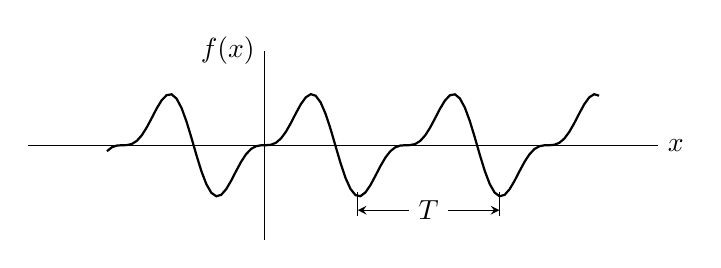
\begin{tikzpicture}
\draw(-3,0)--(5,0)node[right]{$x$};
\draw(0,-1.2)--(0,1.2)node[left]{$f(x)$};
\draw[thick,domain=-400:850,samples=100] plot ({\x/200},{0.5*sin(\x)-0.5/2*sin(2*\x)});
\draw(237/200,-0.6)--++(0,-0.3)coordinate[pos=0.75](kA);
\draw(237/200+360/200,-0.6)--++(0,-0.3)coordinate[pos=0.75](kB);
\draw[stealth-stealth] (kA)--(kB)node[pos=0.5,fill=white]{$T$};
\end{tikzpicture}
\caption{دوری تفاعل}
\label{شکل_فوریئر_دوری_تفاعل}
\end{figure} 

دوری تفاعل کی مثالیں \عددی{\sin x} اور \عددی{\cos x} ہیں۔اس کے علاوہ \عددی{f=c=\text{مستقل}} بھی دوری تفاعل کی تعریف (مساوات \حوالہ{مساوات_فوریئر_دوری_تعریف_الف} پر ہر مثبت \عددی{T} کے لئے) پورا اترنے کی بنا  دوری تفاعل ہے۔

مساوات \حوالہ{مساوات_فوریئر_دوری_تعریف_الف} سے ظاہر ہے کہ عدد صحیح \عددی{n} کی صورت میں درج ذیل ہو گا۔
\begin{align*}
f(x+nT)=f(x)\quad \quad \quad \text{\RL{تمام $x$ کے لئے}}
\end{align*}
یوں \عددی{2T}، \عددی{3T}، \عددی{4T}، \نقطے بھی تفاعل \عددی{f(x)} کے دوری عرصے ہیں۔مزید اگر تفاعل \عددی{f(x)} کا اور \عددی{g(x)} کا دوری عرصہ \عددی{T} ہو تب درج ذیل تفاعل
\begin{align*}
h(x)=af(x)+bg(x)\quad \quad \text{\RL{مستقل $a$، $b$}}
\end{align*}
 کا دوری عرصہ بھی \عددی{T} ہو گا جہاں \عددی{a} اور \عددی{b} مستقل ہیں۔

اس باب کی شروع میں ہم ایسے مختلف تفاعل جن کا دوری عرصہ \عددی{2\pi} ہو کو درج ذیل سادہ تفاعل کی  روپ میں ظاہر کرنا سیکھیں گے
\begin{align*}
1,\quad \cos x,\, \sin x,\quad \cos 2x,\, \sin 2x,\,\cdots, \quad \cos nx,\, \sin nx,\,\cdots
\end{align*}
جن کا دوری عرصہ \عددی{2\pi} ہے (شکل \حوالہ{شکل_فوریئر_سائن_کوسائن_یکساں_دوری_عرصہ})۔ہم دیکھیں گے کہ  ایسا کرتے ہوئے درج ذیل طرز کی تسلسل حاصل ہو گی
\begin{align}\label{مساوات_فوریئر_دوری_تعریف_ب}
a_0+a_1\cos x+b_1\sin x+a_2\cos 2x+b_2\sin 2x+\cdots
\end{align}
جہاں \عددی{a_0}، \عددی{a_1}، \عددی{a_2}،\نقطے، \عددی{b_1}،\عددی{b_2}،\نقطے حقیقی مستقل ہوں گے۔اس تسلسل کو \اصطلاح{تکونیاتی تسلسل}\فرہنگ{تسلسل!تکونیاتی}\حاشیہب{trigonometric series}\فرہنگ{series!trigonometric} کہتے ہیں جبکہ \عددی{a_n} اور \عددی{b_n} تسلسل کی \اصطلاح{عددی سر}\فرہنگ{عددی سر}\حاشیہب{coefficients}\فرہنگ{coefficients} کہلاتے ہیں۔چونکہ اس تسلسل کے ہر رکن کا دوری عرصہ \عددی{2\pi} ہے لہٰذا اگر یہ تسلسل مرکوز ہو تب یہ ایسا تفاعل ہو گا جس کا دوری عرصہ \عددی{2\pi} ہو گا۔
 
\begin{figure}
\centering
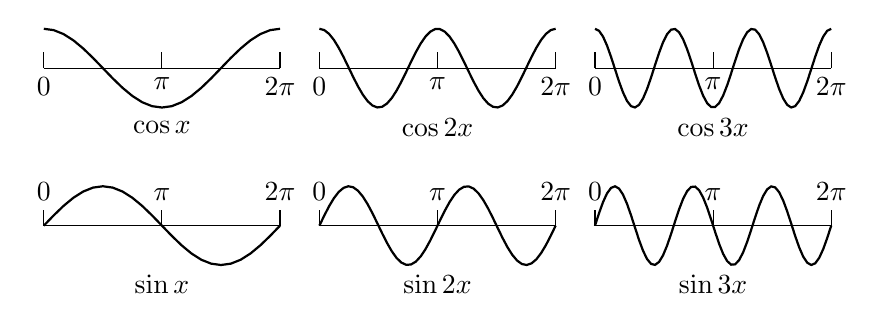
\begin{tikzpicture}
\pgfmathsetmacro{\amp}{0.5}
\pgfmathsetmacro{\pp}{120}
%
\draw(0,0)--(360/\pp,0);
\foreach \x/\l in {0/0,1.5/\pi,3/2\pi}{\draw(\x,0)node[below]{$\l$}--++(0,0.2);}
\draw[thick,domain=0:360] plot ({\x/\pp},{\amp*cos(\x)});
\draw(1.5,-1.5*\amp)node{$\cos x$};
%
\begin{scope}[shift={(0,-4*\amp)}]
\draw(0,0)--(360/\pp,0);
\foreach \x/\l in {0/0,1.5/\pi,3/2\pi}{\draw(\x,0)--++(0,0.2)node[above]{$\l$};}
\draw[thick,domain=0:360] plot ({\x/\pp},{\amp*sin(\x)});
\draw(1.5,-1.5*\amp)node{$\sin x$};
\end{scope}
%===========================
\begin{scope}[shift={(3.5,0)}]
\draw(0,0)--(360/\pp,0);
\foreach \x/\l in {0/0,1.5/\pi,3/2\pi}{\draw(\x,0)node[below]{$\l$}--++(0,0.2);}
\draw[thick,domain=0:360,samples=50] plot ({\x/\pp},{\amp*cos(2*\x)});
\draw(1.5,-1.5*\amp)node{$\cos 2x$};
%
\begin{scope}[shift={(0,-4*\amp)}]
\draw(0,0)--(360/\pp,0);
\foreach \x/\l in {0/0,1.5/\pi,3/2\pi}{\draw(\x,0)--++(0,0.2)node[above]{$\l$};}
\draw[thick,domain=0:360,samples=50] plot ({\x/\pp},{\amp*sin(2*\x)});
\draw(1.5,-1.5*\amp)node{$\sin 2x$};
\end{scope}
\end{scope}
%================================
\begin{scope}[shift={(7,0)}]
\draw(0,0)--(360/\pp,0);
\foreach \x/\l in {0/0,1.5/\pi,3/2\pi}{\draw(\x,0)node[below]{$\l$}--++(0,0.2);}
\draw[thick,domain=0:360,samples=60] plot ({\x/\pp},{\amp*cos(3*\x)});
\draw(1.5,-1.5*\amp)node{$\cos 3x$};
%
\begin{scope}[shift={(0,-4*\amp)}]
\draw(0,0)--(360/\pp,0);
\foreach \x/\l in {0/0,1.5/\pi,3/2\pi}{\draw(\x,0)--++(0,0.2)node[above]{$\l$};}
\draw[thick,domain=0:360,samples=60] plot ({\x/\pp},{\amp*sin(3*\x)});
\draw(1.5,-1.5*\amp)node{$\sin 3x$};
\end{scope}
\end{scope}
\end{tikzpicture}
\caption{سائن اور کوسائن تفاعل جن کا دوری عرصہ $2\pi$ ہے}
\label{شکل_فوریئر_سائن_کوسائن_یکساں_دوری_عرصہ}
\end{figure}

انجینئری میں واقع تفاعل پیچیدہ  ہوتے ہیں جنہیں سادہ دوری تفاعل کی روپ میں لکھنا مدد گار ثابت ہوتا ہے۔ہم دیکھیں گے کہ عملی استعمال، مثلاً ارتعاش، میں پائے جانے والا  تقریباً ہر دوری تفاعل \عددی{f(x)} جس کا دوری عرصہ \عددی{2\pi} ہو  کو فوریئر تسلسل کی روپ میں لکھنا ممکن ہو گا۔ہم مساوات \حوالہ{مساوات_فوریئر_دوری_تعریف_ب} کے عددی سر حاصل کرنے کے ایسے کلیات دریافت کریں گے جو \عددی{f(x)} پر منحصر ہوں گے اور جنہیں استعمال کرتے ہوئے حاصل تسلسل مرکوز ہو گا جس کا مجموعہ \عددی{f(x)} کے برابر ہو گا۔اس کے بعد ہم حاصل کلیات کو عمومی شکل دیتے ہوئے ان  کو کسی بھی دوری عرصہ کے تفاعل کے لئے قابل استعمال بنائیں گے۔ایسا کرنا نہایت آسان ثابت ہو گا۔

%============================
\حصہء{سوالات}

%===================
\ابتدا{سوال}\شناخت{سوال_فوریئر_کمتر_دوری_عرصہ_الف}\quad دیے گئے تفاعل کا کم تر دوری عرصہ دریافت کریں۔
\begin{align*}
\cos x,\, \sin x,\, \cos 2x,\, \sin 2x,\, \cos \pi x,\, \sin \pi x,\, \cos 2\pi x,\, \sin 2\pi x
\end{align*}
جوابات:\quad
$2\pi, 2\pi,\pi, \pi,2,2,1,1$

\انتہا{سوال}
%======================
\ابتدا{سوال}\quad اگر تفاعل \عددی{f(x)} کا دوری عرصہ \عددی{T} ہو تب ثابت کریں کہ \عددی{nT} جہاں \عددی{n=2,3,\cdots} ہے بھی اس تفاعل کا دوری عرصہ ہو گا۔
\انتہا{سوال}
%=====================
\ابتدا{سوال}\quad ثابت کریں کہ اگر تفاعل \عددی{f(x)} کا  اور تفاعل \عددی{g(x)} کا دوری عرصہ \عددی{T} ہو تب تفاعل \عددی{h(x)=af(x)+bg(x)} کا دوری عرصہ بھی \عددی{T} ہو گا، جہاں \عددی{a} اور \عددی{b} مستقل ہیں۔یوں دوری عرصہ \عددی{T} رکھنے والے تمام تفاعل سمتی فضا پیدا کرتے ہیں۔
\انتہا{سوال}
%=====================
\ابتدا{سوال}\quad ثابت کریں کہ تفاعل \عددی{f(x)=\text{مستقل}} ایسا دوری تفاعل ہے جس کا دوری عرصہ \عددی{T} کوئی بھی مثبت عدد ہو سکتا ہے۔
\انتہا{سوال}
%========================
\ابتدا{سوال}\quad ثابت کریں کہ  تفاعل \عددی{f(x)} کا دوری عرصہ \عددی{T} ہونے کی صورت میں \عددی{x} کے دوری تفاعل  \عددی{f(ax), a\ne 0} کا دوری عرصہ \عددی{\tfrac{T}{a}} ہو گا جبکہ \عددی{x} کے دوری  تفاعل \عددی{f(\tfrac{x}{b}), b\ne 0}  کا دوری عرصہ \عددی{bT} ہو گا۔ان نتائج کی تصدیق \عددی{f(x)=\cos x,\, a=b=2} کے لئے کریں۔ 
\انتہا{سوال}
%========================
سوال \حوالہ{سوال_فوریئر_ترسیم_کھینچیں_الف} تا سوال \حوالہ{سوال_فوریئر_ترسیم_کھینچیں_ب} میں دیے گئے تفاعل کا ترسیم کھینچیں۔

%===============
\ابتدا{سوال}\شناخت{سوال_فوریئر_ترسیم_کھینچیں_الف}\quad
$\sin x,\quad \sin x+\frac{1}{3}\sin 3x,\quad \sin x+\frac{1}{3}\sin 3x+\frac{1}{5}\sin 5x$

\انتہا{سوال}
%==========================
\ابتدا{سوال}\quad \عددی{f(x+2\pi)=f(x)} اور
\begin{align*}
f(x)=
\begin{cases}
-\frac{\pi}{4}& -\pi \le x \le 0\\
\phantom{-}\frac{\pi}{4}&\phantom{-}0\le x \le \pi
\end{cases}
\end{align*}
ہے۔سوال \حوالہ{سوال_فوریئر_ترسیم_کھینچیں_الف} کی ترسیم کے ساتھ موازنہ کریں۔
\انتہا{سوال}
%======================
\ابتدا{سوال}
\begin{align*}
\sin 2\pi x,\quad \sin 2\pi x+\frac{1}{3}\sin 6\pi x,\quad \sin 2\pi x+\frac{1}{3}\sin 6\pi x+\frac{1}{5}\sin 10\pi x
\end{align*}
\انتہا{سوال}
%========================
\ابتدا{سوال}
\begin{align*}
\sin x,\quad \sin x-\frac{1}{2}\sin 2x,\quad \sin x-\frac{1}{2}\sin 2x+\frac{1}{3}\sin 3x,\\
f(x)=\frac{x}{2}, \quad  -\pi \le x \le \pi, \quad f(x+2\pi)=f(x)
\end{align*}
\انتہا{سوال}
%========================
\ابتدا{سوال}
\begin{align*}
-\cos x,\quad -\cos x+\frac{1}{4}\cos 2x,\quad -\cos x+\frac{1}{4}\cos 2x-\frac{1}{9}\cos 3x,\\
f(x)=\frac{x^2}{4}-\frac{\pi^2}{12}, \quad  -\pi \le x \le \pi, \quad f(x+2\pi)=f(x)
\end{align*}
\انتہا{سوال}
%================================
\ابتدا{سوال}\quad 
$f(x)=x^2,\quad -\pi \le x \le \pi, \quad f(x+2\pi)=f(x)$
\انتہا{سوال}
%=======================
\ابتدا{سوال}\شناخت{سوال_فوریئر_ترسیم_کھینچیں_ب}\quad 
$f(x)=e^{\abs{x}},\quad -\pi \le x \le \pi, \quad f(x+2\pi)=f(x)$
\انتہا{سوال}
%=======================
سوال \حوالہ{سوال-فوریئر_دوری_تفاعل_الف} تا سوال \حوالہ{سوال-فوریئر_دوری_تفاعل_ب} میں دوری تفاعل \عددی{f(x)} دیا گیا ہے جس کا دوری عرصہ \عددی{2\pi} ہے۔اس کی ترسیم کھینچیں۔وقفہ \عددی{-\pi\le x\le \pi} کے لئے \عددی{f(x)} دیا گیا ہے۔

%=======================
\ابتدا{سوال}\شناخت{سوال-فوریئر_دوری_تفاعل_الف}
\begin{align*}
f(x)=
\begin{cases}
x^2&-\pi \le x\le 0\\
0& \phantom{-}0 \le x \le \pi
\end{cases}
\end{align*}
\انتہا{سوال}
%========================
\ابتدا{سوال}
\begin{align*}
f(x)=
\begin{cases}
0&-\pi \le x\le 0\\
\cos x& \phantom{-}0 \le x \le \pi
\end{cases}
\end{align*}
\انتہا{سوال}
%========================
\ابتدا{سوال}
\begin{align*}
f(x)=
\begin{cases}
\pi+x&-\pi \le x\le 0\\
\pi-x& \phantom{-}0 \le x \le \pi
\end{cases}
\end{align*}
\انتہا{سوال}
%========================
\ابتدا{سوال}\شناخت{سوال-فوریئر_دوری_تفاعل_ب}
\begin{align*}
f(x)=
\begin{cases}
0&-\pi \le x\le 0\\
\sin \frac{x}{2}& \phantom{-}0 \le x \le \pi
\end{cases}
\end{align*}
\انتہا{سوال}
%========================
سوال \حوالہ{سوال_فوریئر_درکار_تکمل_الف} تا سوال \حوالہ{سوال_فوریئر_درکار_تکمل_ب} میں دیے گئے تکمل ہمیں آگے درکار ہوں گے۔ان تکمل میں \عددی{n=0,1,2,\cdots} ہے۔تکمل کی قیمت دریافت کریں۔

%===========================
\ابتدا{سوال}\شناخت{سوال_فوریئر_درکار_تکمل_الف}\quad
$\int\limits_0^{\pi}\sin nx\,\dif x$\\
جواب:\quad طاق \عددی{n} کے لئے \عددی{\tfrac{2}{n}} اور جفت \عددی{n} کے لئے صفر۔
\انتہا{سوال}
%============================
\ابتدا{سوال}\quad
$\int\limits_{-\frac{\pi}{2}}^0\cos nx\,\dif x$\\
جواب:\quad جفت \عددی{n} کے لئے صفر اور طاق \عددی{n} کے لئے \عددی{\tfrac{1}{n}\sin\tfrac{n\pi}{2}}
\انتہا{سوال}
%============================
\ابتدا{سوال}\quad
$\int\limits_{-\pi}^{\pi}x\sin nx\,\dif x$\\
جواب:\quad 
$(-1)^{n+1}\tfrac{2\pi}{n}$
\انتہا{سوال}
%============================
\ابتدا{سوال}\quad
$\int\limits_{-\frac{\pi}{2}}^{\frac{\pi}{2}}x\sin nx\,\dif x$\\
جواب:\quad طاق \عددی{n}، \عددی{\tfrac{2}{n^2}\sin \tfrac{n\pi}{2}} یعنی \عددی{(-1)^{\tfrac{n+3}{2}}\tfrac{2}{n^2}} جبکہ جفت \عددی{n}، \عددی{-\tfrac{\pi}{n}\cos\tfrac{n\pi}{2}} یعنی \عددی{(-1)^{\tfrac{n+2}{2}}\tfrac{\pi}{n}}
\انتہا{سوال}
%============================
\ابتدا{سوال}\quad
$\int\limits_{-\frac{\pi}{2}}^{\frac{\pi}{2}}x\cos nx\,\dif x$\\
جواب:\quad 
$0$
\انتہا{سوال}
%============================
\ابتدا{سوال}\quad
$\int\limits_{0}^{\pi}x\sin nx\,\dif x$\\
جواب:\quad
$\tfrac{\pi}{n}(-1)^{n+1}$
\انتہا{سوال}
%============================
\ابتدا{سوال}\quad
$\int\limits_{-\pi}^{0} e^x\sin nx\,\dif x$\\
جواب:\quad
$\tfrac{n}{n^2+1}[(-1)^ne^{-\pi}-1]$
\انتہا{سوال}
%============================
\ابتدا{سوال}\quad
$\int\limits_{0}^{\pi} e^x\cos nx\,\dif x$\\
جواب:\quad
$\tfrac{1}{n^2+1}[e^{\pi}(-1)^n-1]$
\انتہا{سوال}
%============================
\ابتدا{سوال}\شناخت{سوال_فوریئر_درکار_تکمل_ب}\quad
$\int\limits_{-\pi}^{\pi} x^2\cos nx\,\dif x$\\
جواب:\quad
$\tfrac{4\pi}{n^2}(-1)^n$
\انتہا{سوال}
%============================

\حصہ{فوریئر تسلسل۔ یولر کلیات}\شناخت{حصہ_فوریئر_یولر_کلیات}
فرض کریں کہ دوری تفاعل \عددی{f(x)} جس کا دوری عرصہ \عددی{2\pi} ہے کو درج ذیل تکونیاتی تسلسل سے ظاہر کیا جا سکتا ہے۔
\begin{align}\label{مساوات_فوریئر_تسلسل_الف}
f(x)=a_0+\sum_{n=1}^{\infty}(a_n\cos nx+b_n\sin nx)
\end{align}
ہم دیے گئے تفاعل \عددی{f(x)} کی تکونیاتی تسلسل (مساوات \حوالہ{مساوات_فوریئر_تسلسل_الف}) کے عددی سر \عددی{a_n}، اور \عددی{b_n} جاننا چاہتے ہیں۔

ہم سب سے پہلے \عددی{a_0} دریافت کرتے ہیں۔مساوات \حوالہ{مساوات_فوریئر_تسلسل_الف} کے دونوں اطراف کا \عددی{-\pi} تا \عددی{\pi} تکمل لیتے ہیں۔
\begin{align*}
\int_{-\pi}^{\pi}f(x)\,\dif x=\int_{-\pi}^{\pi}\big[a_0+\sum_{n=1}^{\infty}(a_n\cos nx+b_n\sin nx)\big]\dif x
\end{align*}
اگر تسلسل کے ارکان کا جزو با جزو تکمل لینا جائز ہو\حاشیہد{ایسا جائز ہے، مثلاً، استمراری مرتکز صورت میں۔}، تب درج ذیل لکھا جا سکتا ہے۔
\begin{align*}
\int_{-\pi}^{\pi}f(x)\,\dif x=a_0\int_{-\pi}^{\pi}\dif x+ \sum_{n=1}^{\infty}\big(a_n\int_{-\pi}^{\pi}\cos nx\,\dif x+b_n\int_{-\pi}^{\pi}\sin nx \,\dif x\big)
\end{align*}
دائیں ہاتھ پہلا رکن \عددی{2\pi a_0} کے برابر ہے۔بائیں ہاتھ باقی تمام ارکان صفر کے برابر ہیں، جیسا کہ تکمل لے کر ثابت کیا جا سکتا ہے۔یوں پہلا کلیہ درج ذیل ملتا ہے۔
\begin{align}\label{مساوات_فوریئر_تسلسل_ب}
a_0=\frac{1}{2\pi}\int_{-\pi}^{\pi}f(x)\,\dif x
\end{align}

ہم اب \عددی{a_1}، \عددی{a_2}، \نقطے اسی طرح حاصل کرتے ہیں۔ہم مساوات \حوالہ{مساوات_فوریئر_تسلسل_الف} کو \عددی{\cos mx} سے ضرب دیتے ہوئے، جہاں \عددی{m} کوئی مقررہ مثبت عدد صحیح ہے، دونوں اطراف کا \عددی{-\pi} تا \عددی{\pi} تکمل لیتے ہیں۔
\begin{align}\label{مساوات_فوریئر_تسلسل_پ}
\int_{-\pi}^{\pi}f(x)\cos mx\,\dif x=\int_{-\pi}^{\pi}\big[a_0+\sum_{n=1}^{\infty}(a_n\cos nx+b_n\sin nx)\big]\cos mx\, \dif x
\end{align}
جزو در جزو تکمل لیتے ہوئے  دائیں ہاتھ کو درج ذیل لکھا جا سکتا ہے۔
\begin{align*}
a_0\int_{-\pi}^{\pi}\cos mx\,\dif x+\sum_{n=1}^{\infty}\big[a_n\int_{-\pi}^{\pi}\cos nx\,\cos mx\,\dif x+b_n\int_{-\pi}^{\pi}\sin nx\,\cos mx\,\dif x\big]
\end{align*}
پہلا تکمل صفر کے برابر ہے۔ضمیمہ-\حوالہ{ضمیمہ_مفید_معلومات} میں دیا گیا مساوات \حوالہ{مساوات_ضمیمہ_مفید_گیارہ} استعمال کرتے ہوئے درج ذیل لکھا جا سکتا ہے۔
\begin{gather*}
\begin{aligned}
\int_{-\pi}^{\pi} \cos nx\,\cos mx\,\dif x&=\frac{1}{2}\int_{-\pi}^{\pi}\cos(n+m)x\,\dif x
+\frac{1}{2}\int_{-\pi}^{\pi} \cos (n-m)x\,\dif x\\
\int_{-\pi}^{\pi} \sin nx\,\cos mx\,\dif x&=\frac{1}{2}\int_{-\pi}^{\pi}\sin(n+m)x\,\dif x+\frac{1}{2}\int_{-\pi}^{\pi} \sin (n-m)x\,\dif x
\end{aligned}
\end{gather*}
تکمل لینے سے ثابت ہوتا ہے کہ بالائی دائیں جزو کے علاوہ تمام تکمل صفر کے برابر ہیں۔بالائی دایاں جزو \عددی{n=m} کی صورت میں \عددی{\pi} کے برابر ہے۔چونکہ مساوات \حوالہ{مساوات_فوریئر_تسلسل_پ} میں اس جزو کو \عددی{a_n} ضرب کرتا ہے (جس کو \عددی{n=m} کی بنا \عددی{a_m} لکھا جا سکتا ہے) لہٰذا مساوات \حوالہ{مساوات_فوریئر_تسلسل_پ} کا دایاں ہاتھ \عددی{a_m\pi} کے برابر ہو گا۔یوں دوسرا کلیہ درج ذیل حاصل ہوتا ہے۔
\begin{align}\label{مساوات_فوریئر_تسلسل_ت}
a_m=\frac{1}{\pi}\int_{-\pi}^{\pi}f(x)\cos mx\,\dif x,\quad \quad m=1,2,\cdots
\end{align}

ہم آخر میں \عددی{b_1}، \عددی{b_2}، \نقطے حاصل کرتے ہیں۔مساوات \حوالہ{مساوات_فوریئر_تسلسل_الف} کو \عددی{\sin mx} سے ضرب دیتے ہوئے، جہاں \عددی{m} کوئی مثبت مقررہ عدد صحیح  ہے، \عددی{-\pi} تا \عددی{\pi} تکمل لیتے ہیں۔
\begin{align}\label{مساوات_فوریئر_تسلسل_ٹ}
\int_{-\pi}^{\pi}f(x)\sin mx\,\dif x=\int_{-\pi}^{\pi}\big[a_0+\sum_{n=1}^{\infty}(a_n\cos nx+b_n\sin nx) \big]\sin mx\, \dif x
\end{align}
جزو در جزو تکمل لیتے ہوئے دایاں ہاتھ درج ذیل لکھا جا سکتا ہے۔
\begin{align*}
a_0\int_{-\pi}^{\pi}\sin mx\,\dif x+\sum_{n=1}^{\infty}\big[a_n\int_{-\pi}^{\pi}\cos nx\,\sin mx\,\dif x+b_n\int_{-\pi}^{\pi}\sin nx\,\sin mx\,\dif x\big]
\end{align*}
پہلا تکمل صفر کے برابر ہے۔دوسرے تکمل کی طرز کی تکمل پر ہم غور کر چکے ہیں اور ہم جانتے ہیں کہ تمام \عددی{n=1,2,\cdots} کے لئے اس کی قیمت صفر ہے۔آخری تکمل کو ہم درج ذیل لکھ سکتے ہیں۔
\begin{align*}
\int_{-\pi}^{\pi}\sin nx \,\sin mx\,\dif x=\frac{1}{2}\int_{-\pi}^{\pi}\cos(n-m)\,\dif x-\frac{1}{2}\int_{-\pi}^{\pi}\cos(n+m)\,\dif x
\end{align*}
آخری جزو صفر کے برابر ہے۔دائیں ہاتھ پہلا جزو \عددی{n\ne m} کی صورت میں صفر جبکہ \عددی{n=m} کی صورت میں \عددی{\pi} کے برابر ہے۔ چونکہ مساوات \حوالہ{مساوات_فوریئر_تسلسل_ٹ} میں اس جزو کو \عددی{b_n} ضرب کرتا ہے (جس کو \عددی{n=m} کی بنا \عددی{b_m} لکھا جا سکتا ہے) لہٰذا مساوات \حوالہ{مساوات_فوریئر_تسلسل_ٹ}  کا دایاں ہاتھ \عددی{b_m\pi} کے برابر ہو گا۔یوں آخری کلیہ درج ذیل حاصل ہوتا ہے۔
\begin{align}\label{مساوات_فوریئر_تسلسل_ث}
b_m=\frac{1}{\pi}\int_{-\pi}^{\pi}f(x)\sin mx\,\dif x,\quad \quad m=1,2,\cdots
\end{align}
اب \عددی{m} کی جگہ \عددی{n} لکھتے ہوئے ان کلیات کو، جنہیں \اصطلاح{یولر کلیات}\فرہنگ{یولر!کلیات}\حاشیہب{Euler formulas}\فرہنگ{Euler!formulas} کہتے، ایک جگہ اکٹھا کرتے ہیں۔ 
\begin{gather}
\begin{aligned}\label{مساوات_فوریئر_تسلسل_ج}
\text{(الف)}\quad \quad a_0&=\frac{1}{2\pi}\int_{-\pi}^{\pi}f(x)\,\dif x\\
\text{(ب)}\quad \quad a_n&=\frac{1}{\pi}\int_{-\pi}^{\pi}f(x)\cos nx\,\dif x,\quad \quad n=1,2,\cdots\\
\text{(پ)}\quad \quad b_n&=\frac{1}{\pi}\int_{-\pi}^{\pi}f(x)\sin nx\,\dif x,\quad \quad n=1,2,\cdots
\end{aligned}
\end{gather}

چونکہ متکمل دوری ہیں لہٰذا مساوات \حوالہ{مساوات_فوریئر_تسلسل_ج} میں وقفہ تکمل کو \عددی{2\pi} کے برابر کسی بھی وقفہ، مثلاً \عددی{0\le x\le 2\pi}،  سے بدلا جا سکتا ہے۔

دوری تفاعل \عددی{f(x)} جس کا دوری عرصہ \عددی{2\pi} ہو کو استعمال کرتے ہوئے مساوات \حوالہ{مساوات_فوریئر_تسلسل_ج} کی مدد سے عددی سر \عددی{a_n} اور \عددی{b_n} حاصل کر کے ہم درج ذیل تکونیاتی تسلسل لکھتے ہیں۔
\begin{align}\label{مساوات_فوریئر_تسلسل_تفاعل_کی}
a_0+a_1\cos x+b_1\sin x+\cdots+a_n\cos nx+b_n\sin nx+\cdots
\end{align}
اس تسلسل کو \عددی{f(x)} کی \اصطلاح{فوریئر تسلسل}\فرہنگ{تسلسل!فوریئر}\فرہنگ{فوریئر!تسلسل}\حاشیہب{Fourier series}\فرہنگ{Fourier!series} کہتے ہیں جبکہ مساوات \حوالہ{مساوات_فوریئر_تسلسل_ج} سے حاصل عددی سر \عددی{a_n}، \عددی{b_n} کو \عددی{f(x)} کے \اصطلاح{فوریئر عددی سر}\فرہنگ{فوریئر!عددی سر}\حاشیہب{Fourier coefficients}\فرہنگ{Fourier!coefficients} کہتے ہیں۔

قطعی تکمل کی تعریف سے واضح ہے کہ اگر \عددی{f(x)} استمراری یا ٹکڑوں میں استمراری (جہاں وقفہ تکمل پر \عددی{f(x)} میں محدود تعداد کے چھلانگ پائے جاتے ہوں) ہو تب مساوات \حوالہ{مساوات_فوریئر_تسلسل_ج} میں دیے گئے تکملات موجود ہوں گے لہٰذا ہم \عددی{f(x)} کے فوریئر عددی سروں کو مساوات \حوالہ{مساوات_فوریئر_تسلسل_ج} کی مدد سے حاصل کر سکتے ہیں۔اب سوال پیدا ہوتا ہے کہ آیا اس طرح حاصل کیا گیا فوریئر تسلسل مرکوز ہو گا اور آیا تسلسل کا مجموعہ \عددی{f(x)} کے برابر ہو گا؟  ان سوالات پر اسی حصے میں آگے جا کر غور کیا جائے گا۔

آئیں مساوات \حوالہ{مساوات_فوریئر_تسلسل_ج} کی استعمال کو ایک سادہ مثال کی مدد سے سمجھیں۔

%========================
\ابتدا{مثال}\شناخت{مثال_فوریئر_چکور_موج}\quad چکور موج\\
چکور موج کے فوریئر عددی سر کو مساوات \حوالہ{مساوات_فوریئر_تسلسل_ج} سے حاصل کریں۔چکور موج کو شکل \حوالہ{شکل_مثال_فوریئر_چکور_موج}-الف میں دکھایا گیا ہے۔چکور موج کی تحلیلی روپ درج ذیل ہے۔
\begin{align*}
f(x)=
\begin{cases}
-k& -\pi< x <0\\
\phantom{-}k & \phantom{-}0< x < \pi
\end{cases}
\quad \text{جہاں}\quad f(x+2\pi)=f(x)
\end{align*}
اس طرز کے تفاعل میکانی نظام میں بطور بیرونی قوت یا برقی ادوار میں بطور داخلی دباو پائے جا سکتے ہیں، وغیرہ۔
% 
\begin{figure}
\centering
\begin{subfigure}{1\textwidth}
\centering
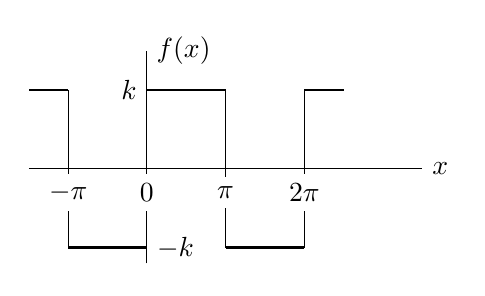
\begin{tikzpicture}
\pgfmathsetmacro{\T}{1}
\draw(-1.5,0)--(3.5,0)node[right]{$x$};
\draw(0,-1.2)--(0,1.5)node[right]{$f(x)$};
%square wave
\draw[thick](0,1)node[left]{$k$}--++(\T,0)++(\T,0)--++(\T/2,0);
\draw[thick](-\T,1)--++(-\T/2,0);
\draw[thick](-\T,-1)--++(\T,0)node[right]{$-k$}++(\T,0)--++(\T,0);
\draw(-\T,1)--++(0,-2);
\draw(\T,1)--++(0,-2);
\draw(2*\T,1)--++(0,-2);
%ticks
\foreach \x/\l in {-1/-\pi,0/0,1/\pi,2/2\pi}{\draw(\x,0)node[fill=white,shift={(0,-0.3)}]{$\l$};}
\end{tikzpicture}
\caption*{(الف) دیا گیا دوری چکور تفاعل $f(x)$}
\end{subfigure}
\begin{subfigure}{1\textwidth}
\centering
\begin{tikzpicture}
\pgfmathsetmacro{\w}{45}
\draw(-4.4,0)--(6,0)node[right]{$x$};
\draw(0,-1.5)--(0,1.5);
%
\draw(0,1)node[left]{$k$}--++(4,0);
\draw(0,-1)node[right]{$-k$}--++(-4,0);
\draw[domain=-180:180,smooth,thick] plot ({\x/\w},{1.273*sin(\x)});
\draw[stealth-] ({100/\w},{1.273*sin(100)}) to [out=45,in=180]++(0.5,0.25)node[right]{$S_1$};
%text
\draw(-4,0)--++(0,-0.2)node[shift={(-0.25,-0.2)}]{$-\pi$};
\draw(4,0)--++(0,-0.2)node[below ]{$\pi$};;
\end{tikzpicture}
\caption*{(ب)}
\end{subfigure}
\begin{subfigure}{1\textwidth}
\centering
\begin{tikzpicture}
\pgfmathsetmacro{\w}{45}
\draw(-4.4,0)--(6,0)node[right]{$x$};
\draw(0,-1.5)--(0,1.5);
%
\draw(0,1)node[left]{$k$}--++(4,0);
\draw(0,-1)node[right]{$-k$}--++(-4,0);
\draw[domain=0:180,smooth,dashed] plot ({\x/\w},{1.273*sin(\x)});
\draw[domain=0:180,smooth,dashed] plot ({\x/\w},{1.273*(1/3*sin(3*\x))});
\draw[domain=-180:180,samples=60,thick] plot ({\x/\w},{1.273*(sin(\x)+1/3*sin(3*\x))});
%
\draw[stealth-] ({100/\w},{1.273*sin(100)}) to [out=45,in=180]++(0.5,0.5)node[right]{$S_1$};
\draw[stealth-] ({140/\w},{1.273*(sin(140)+1/3*sin(3*140))}) to [out=45,in=180]++(0.5,0.25)node[right]{$S_3$};
\draw[stealth-] ({90/\w},{1.273*(1/3*sin(3*90)}) to [out=-90,in=180]++(0.25,-0.25)node[right]{$\tfrac{4k}{3\pi}\sin 3x$};
%text
\draw(-4,0)--++(0,-0.2)node[shift={(-0.25,-0.2)}]{$-\pi$};
\draw(4,0)--++(0,-0.2)node[below ]{$\pi$};
\end{tikzpicture}
\caption*{(پ)}
\end{subfigure}
\begin{subfigure}{1\textwidth}
\centering
\begin{tikzpicture}
\pgfmathsetmacro{\w}{45}
\draw(-4.4,0)--(6,0)node[right]{$x$};
\draw(0,-1.5)--(0,1.5);
%
\draw(0,1)node[left]{$k$}--++(4,0);
\draw(0,-1)node[right]{$-k$}--++(-4,0);
\draw[domain=0:180,smooth,dashed] plot ({\x/\w},{1.273*(sin(\x)+1/3*sin(3*\x))});
\draw[domain=0:180,smooth,dashed] plot ({\x/\w},{1.273*(1/5*sin(5*\x))});
\draw[domain=-180:180,samples=100,thick] plot ({\x/\w},{1.273*(sin(\x)+1/3*sin(3*\x)+1/5*sin(5*\x))});
%text
\draw[stealth-] ({50/\w},{1.273*(1/5*sin(5*50))}) to [out=-70,in=180]++(0.5,-0.5)node[right]{$\tfrac{4k}{5\pi}\sin 5x$};
\draw[stealth-]  ({45/\w},{1.273*(sin(45)+1/3*sin(3*45))}) to [out=90,in=180]++(0.5,0.5)node[right]{$S_2$};
\draw[stealth-] ({90/\w},{1.273*(sin(90)+1/3*sin(3*90)+1/5*sin(5*90))}) to [out=90,in=180] ++(0.5,0.5)node[right]{$S_3$};
%
\draw(-4,0)--++(0,-0.2)node[shift={(-0.25,-0.2)}]{$-\pi$};
\draw(4,0)--++(0,-0.2)node[below ]{$\pi$};
\end{tikzpicture}
\caption*{(ت)}
\end{subfigure}
\caption{چکور موج اور فوریئر تسلسل سے حاصل امواج (مثال \حوالہ{مثال_فوریئر_چکور_موج})}
\label{شکل_مثال_فوریئر_چکور_موج}
\end{figure}

حل:مساوات \حوالہ{مساوات_فوریئر_تسلسل_ج}-الف سے \عددی{a_0=0} ملتا ہے۔یہ نتیجہ بغیر تکمل کے یوں حاصل کیا جا سکتا ہے کہ چکور موج کا رقبہ \عددی{-\pi} تا \عددی{\pi} صفر ہے۔مساوات \حوالہ{مساوات_فوریئر_تسلسل_ج}-ب سے
\begin{align*}
a_n=\frac{1}{\pi}\int_{-\pi}^{\pi}f(x)\cos nx\, \dif x&=\frac{1}{\pi}\big[\int_{-\pi}^{0}(-k)\cos nx\,\dif x+\int_{0}^{\pi}k\cos nx\,\dif x\big]\\
&=\frac{1}{\pi}\Big[\left. -k\frac{\sin nx}{n}\right|_{-\pi}^{0}+\left. k\frac{\sin nx}{n}\right|_{0}^{\pi}\Big]=0
\end{align*}
ملتا ہے جہاں تمام \عددی{n=1,2,\cdots} کے لئے \عددی{-\pi}، \عددی{0} اور \عددی{\pi} پر \عددی{\sin nx=0}  پر کیا گیا ہے۔اسی طرح مساوات \حوالہ{مساوات_فوریئر_تسلسل_ج}-پ سے
\begin{align*}
b_n=\frac{1}{\pi}\int_{-\pi}^{\pi}f(x)\sin nx\, \dif x&=\frac{1}{\pi}\big[\int_{-\pi}^{0}(-k)\sin nx\,\dif x+\int_{0}^{\pi}k\sin nx\,\dif x\big]\\
&=\frac{1}{\pi}\Big[\left. k\frac{\cos nx}{n}\right|_{-\pi}^{0}\left. -k\frac{\cos nx}{n}\right|_{0}^{\pi}\Big]
\end{align*}
ملتا ہے۔چونکہ \عددی{\cos 0=1} اور \عددی{\cos(-\alpha)=\cos \alpha} ہوتا ہے لہٰذا اس سے درج ذیل حاصل ہوتا ہے۔
\begin{align*}
b_n=\frac{k}{n\pi}[\cos 0-\cos(-n\pi)-\cos n\pi +\cos 0]=\frac{2k}{n\pi}(1-\cos n\pi)
\end{align*}
اب \عددی{\cos \pi=-1}، \عددی{\cos 2\pi=1}، \عددی{\cos 3\pi=-1}، وغیرہ سے درج ذیل لکھا جا سکتا ہے۔
\begin{align*}
\cos n\pi=
\begin{cases}
-1& \text{\RL{طاق $n$}}\\
\phantom{-}1&\text{\RL{جفت $n$}}
\end{cases}
\quad \implies \quad
1-\cos n\pi=
\begin{cases}
2&\text{\RL{طاق $n$}}\\
0&\text{\RL{جفت $n$}}
\end{cases}
\end{align*}
یوں \عددی{b_n} درج ذیل ہوں گے۔
\begin{align*}
b_1=\frac{4k}{\pi},\quad  b_2=0,\quad  b_3=\frac{4k}{3\pi},\quad b_4=0,\quad  b_5=\frac{4k}{5\pi}, \cdots
\end{align*}
چونکہ \عددی{a_n=0} ہیں لہٰذا دی گئی چکور تفاعل کی فوریئر تسلسل
\begin{align}
\frac{4k}{\pi}\big(\sin x+\frac{1}{3}\sin 3x+\frac{1}{5}\sin 5x+\cdots \big)
\end{align}
ہو گی جس کے جزوی مجموعے درج ذیل ہیں۔
\begin{align*}
S_1=\frac{4k}{\pi}\sin x,\quad S_2=\frac{4k}{\pi}\big(\sin x+\frac{1}{3}\sin 3x\big),\cdots
\end{align*}
شکل \حوالہ{شکل_مثال_فوریئر_چکور_موج} میں جزوی مجموعہ میں ارکان کی تعداد بتدریج بڑھاتے ہوئے تسلسل کا ترسیم کھینچا  گیا ہے جہاں سے ظاہر ہے کہ تسلسل کے زیادہ ارکان استعمال کرنے سے  ترسیم کی شکل اصل تفاعل (چکور موج) کی زیادہ  قریب ہوتی ہے۔ چکور موج \عددی{-\pi}، \عددی{0}، \عددی{\pi}، وغیرہ پر غیر استمراری ہے یعنی یہاں تفاعل میں چھلانگ پائی جاتی ہے۔یوں ہم نہیں کہہ سکتے کہ آیا \عددی{x=0} پر چکور تفاعل کی قیمت \عددی{-k} ہے یا \عددی{k} ہے  یا کہ ان دونوں قیمتوں کے مابین ہے۔اس کے برعکس فوریئر تسلسل کے تمام جزوی مجموعے ان نقطوں پر صفر کے برابر ہیں جو \عددی{-k} اور \عددی{k} کی اوسط قیمت ہے۔

مزید فرض کریں کہ اس تسلسل کا مجموعہ \عددی{f(x)} کے برابر ہے۔شکل \حوالہ{شکل_مثال_فوریئر_چکور_موج}-الف سے ظاہر ہے کہ \عددی{x=\tfrac{\pi}{2}} پر چکور تفاعل کی قیمت \عددی{k} کے برابر ہے۔یوں \عددی{x=\tfrac{\pi}{2}} پر  کرتے ہوئے
\begin{align*}
f(\frac{\pi}{2})=k\frac{4k}{\pi}\big(1-\frac{1}{3}+\frac{1}{5}-+\cdots\big )
\end{align*}
یعنی
\begin{align}\label{مساوات_فوریئر_لیبنٹز_تعلق}
1-\frac{1}{3}+\frac{1}{5}-\frac{1}{7}+-\cdots=\frac{\pi}{4}
\end{align}
لکھا جا سکتا ہے۔یہ مشہور نتیجہ لیبنٹز نے \عددی{1673} کے لگ بھگ جیومیٹریائی اصولوں سے حاصل کیا۔اس سے آپ دیکھ سکتے ہیں کہ مستقل ارکان کی کئی تسلسل کی قیمت کو  مختلف نقطوں پر فوریئر تسلسل کی قیمت سے حاصل کیا جا سکتا ہے۔  
\انتہا{مثال}
%=======================

ایسے تفاعل جنہیں فوریئر تسلسل سے  ظاہر کرنا ممکن ہو کی تعداد غیر یقینی طور پر زیادہ ہے۔ انجینئری میں استعمال ہونے  والی تقریباً ہر ممکن تفاعل کو فوریئر تسلسل کی صورت میں ظاہر کرنے کے لئے درکار (کافی) شرائط درج ذیل مسئلہ \حوالہ{مسئلہ_فوریئر_مرتکز_شرائط} میں بیان کیے گئے ہیں۔اس مسئلہ میں چند تصورات کی ضرورت ہے جن پر پہلے بات کرتے ہیں۔

نقطہ \عددی{x_0} پر تفاعل \عددی{f(x)} کی \اصطلاح{بائیں ہاتھ حد}\فرہنگ{حد!بائیں ہاتھ}\حاشیہب{left hand limit}\فرہنگ{limit!left hand} سے مراد \عددی{f(x)} کی وہ حد ہے جو \عددی{x_0} تک بائیں ہاتھ سے پہنچتے ہوئے حاصل ہو گی۔یوں بائیں ہاتھ حد جس کو \عددی{f(x_0-1)} سے ظاہر کیا جاتا ہے درج ذیل ہو گی
\begin{align*}
f(x_0-0)=\lim_{h\to 0} f(x_0-h)
\end{align*}
جہاں \عددی{h} مثبت قیمت ہے۔ اسی طرح \عددی{x_0} پر \عددی{f(x)} کی \اصطلاح{دائیں ہاتھ حد}\فرہنگ{حد!دائیں ہاتھ}\حاشیہب{right hand limit}\فرہنگ{limit!right hand} سے مراد \عددی{f(x)} کی وہ حد ہے جو دائیں ہاتھ سے آ کر  \عددی{x_0} تک  پہنچتے ہوئے حاصل ہو گی۔یوں دائیں ہاتھ حد جس کو \عددی{f(x_0+0)} سے ظاہر کیا جاتا ہے
\begin{align*}
f(x_0+0)=\lim_{h\to 0} f(x_0+h)
\end{align*}
ہو گی جہاں \عددی{h} مثبت قیمت ہے۔شکل \حوالہ{شکل_فوریئر_بائیں_ہاتھ_حد} میں  غیر استمراری تفاعل
\begin{align*}
f(x)=
\begin{cases}
x^2& x<1\\
\frac{x}{2}& x>1
\end{cases}
\end{align*}
دکھایا گیا ہے۔نقطہ \عددی{x_0=1} پر اس تفاعل کی بائیں ہاتھ حد اور دائیں ہاتھ حد درج ذیل ہیں
\begin{align*}
f(1-0)=1,\quad f(1+0)=\frac{1}{2}
\end{align*}
جن میں فرق \عددی{(1-\tfrac{1}{2}=\tfrac{1}{2})} کو \اصطلاح{چھلانگ}\فرہنگ{چھلانگ}\حاشیہب{jump}\فرہنگ{jump} کہتے ہیں۔
\begin{figure}
\centering
\begin{tikzpicture}
\draw(0,0)--++(2.5,0)node[below]{$x$};
\draw(0,0)node[ocirc]{}--++(0,1.5)node[left]{$y$};
%
\draw(0,1)node[left]{$1$}--++(0.1,0);
\draw(1,0)node[below]{$1$}--++(0,0.1);
%
\draw[thick,domain=0:1,smooth] plot ({\x},{\x*\x});
\draw[thick,domain=1:2] plot ({\x},{\x/2});
%
\draw[stealth-] (1,1)node[ocirc]{}++(0,0.05) to [out=90,in=180]++(0.5,0.5)node[right]{$f(1-0)$};
\draw(1,1/2)node[ocirc]{}node[shift={(1,0)}]{$f(1+0)$};
\end{tikzpicture}
\caption{بائیں ہاتھ اور دائیں ہاتھ حد، بائیں ہاتھ اور دائیں ہاتھ تفرق}
\label{شکل_فوریئر_بائیں_ہاتھ_حد}
\end{figure}

نقطہ \عددی{x_0} پر \اصطلاح{بائیں ہاتھ تفرق}\فرہنگ{تفرق!بائیں ہاتھ}\فرہنگ{بائیں ہاتھ!تفرق}\حاشیہب{left hand differential}\فرہنگ{differential!left hand} سے مراد
\begin{align*}
\frac{f(x_0-h)-f(x_0-0)}{-h}
\end{align*}
اور \اصطلاح{دائیں ہاتھ تفرق}\فرہنگ{تفرق!دائیں ہاتھ}\فرہنگ{دائیں ہاتھ!تفرق}\حاشیہب{right hand differential}\فرہنگ{differential!right hand} سے مراد
\begin{align*}
\frac{f(x_0+h)-f(x_0+0)}{h}
\end{align*}
ہے جہاں \عددی{h} مثبت قیمت ہے۔ظاہر ہے کہ اگر نقطہ \عددی{x_0} پر تفاعل \عددی{f(x)} استمراری ہو تب \عددی{f(x_0-0)} اور \عددی{f(x_0+0)}  دونوں \عددی{f(x_0)} ہی کے برابر ہوں گے۔

%======================
\ابتدا{مسئلہ}\شناخت{مسئلہ_فوریئر_مرتکز_شرائط}\quad (تفاعل کا فوریئر تسلسل کی روپ میں اظہار)\\
اگر دوری تفاعل \عددی{f(x)} جس کا دوری عرصہ \عددی{2\pi} ہو، وقفہ \عددی{-\pi\le x\le \pi} میں ٹکڑوں میں استمراری\حاشیہد{ٹکڑوں میں استمراری کی تعریف حصہ \حوالہ{حصہ_لاپلاس_بدل_الٹ_بدل_خطیت} میں دی گئی ہے۔} ہو اور اس وقفے کے ہر نقطے پر تفاعل کا دایاں ہاتھ تفرق اور بایاں ہاتھ تفرق موجود ہو تب  تفاعل کی فوریئر تسلسل، مساوات \حوالہ{مساوات_فوریئر_تسلسل_تفاعل_کی}، جس  کی عددی سر  مساوات \حوالہ{مساوات_فوریئر_تسلسل_ج} سے حاصل کیے گئے ہوں، مرتکز ہو گی۔تسلسل کا مجموعہ \عددی{f(x)} کے برابر ہو گا ماسوائے  نقطہ \عددی{x_0} پر جہاں تفاعل غیر استمراری ہو۔نقطہ \عددی{x_0} پر تسلسل کی قیمت،  نقطہ \عددی{x_0} پر \عددی{f(x)} کی بائیں ہاتھ حد اور دائیں ہاتھ حد کی اوسط ہو گی۔ 
\انتہا{مسئلہ}
%========================  
\موٹا{رائے زنی}: اگر تفاعل \عددی{f(x)} کی فوریئر تسلسل مرتکز ہو اور اس تسلسل کا مجموعہ \عددی{f(x)} کے برابر ہو  (جیسا مسئلہ \حوالہ{مسئلہ_فوریئر_مرتکز_شرائط} میں بیان کیا گیا ہے) تب اس تسلسل کو \عددی{ f(x)} کی فوریئر تسلسل کہتے ہیں جس کو ریاضی میں درج ذیل لکھا جاتا ہے
\begin{align*}
f(x)=a_0+a_1\cos x+b_1\sin x+\cdots+a_n\cos nx+b_n\sin nx+\cdots
\end{align*} 
اور ہم کہتے ہیں کہ \عددی{f(x)} کو یہ فوریئر تسلسل ظاہر کرتی ہے۔اب چونکہ کسی بھی مرتکز تسلسل میں قوسین لگانے سے  ایک نئی مرتکز تسلسل ملتی ہے جس کا مجموعہ اصل تسلسل کے مجموعے کے برابر ہوتا ہے لہٰذا ہم درج بالا مساوات کو درج ذیل لکھ سکتے ہیں۔
\begin{align*}
f(x)=a_0+\sum_{n=1}^{\infty}(a_n\cos nx+b_n\sin nx)
\end{align*}
%================
\ابتدا{ثبوت}\quad استمراری تفاعل \عددی{f(x)} جس کا استمراری ایک درجی اور دو درجی تفرق پایا جاتا ہو کی مرکوزیت  (مسئلہ \حوالہ{مسئلہ_فوریئر_مرتکز_شرائط}) کا ثبوت ۔\\
مساوات \حوالہ{مساوات_فوریئر_تسلسل_ج}-ب  کا تکمل بالحصص لیتے ہوئے
\begin{align*}
a_n=\frac{1}{\pi}\int_{-\pi}^{\pi}f(x)\cos nx \,\dif x=\left. \frac{f(x)\sin nx}{n\pi}\right|_{-\pi}^{\pi}-\frac{1}{n\pi}\int_{-\pi}^{\pi} f'(x)\sin nx\,\dif x
\end{align*}
ملتا ہے۔دائیں ہاتھ پہلا جزو صفر کے برابر ہے۔دوبارہ تکمل بالحصص لینے سے
\begin{align*}
a_n=\left.\frac{f'(x)\cos nx}{n^2\pi}\right|_{-\pi}^{\pi}-\frac{1}{n^2\pi}\int_{-\pi}^{\pi} f''(x)\cos nx\, \dif x
\end{align*}
ملتا ہے۔چونکہ \عددی{f'(x)}  دوری اور استمراری ہے لہٰذا دائیں ہاتھ پہلا جزو صفر ہو گا۔ وقفہ تکمل  میں \عددی{f''(x)} استمراری ہے لہٰذا 
\begin{align*}
\abs{f''(x)} <M
\end{align*}
ہو گا جہاں \عددی{M} ایک موزوں مستقل ہے۔مزید \عددی{\abs{\cos nx}<1} ہے۔ یوں
\begin{align*}
\abs{a_n}=\frac{1}{n^2\pi}\abs{\int_{-\pi}^{\pi} f''(x) \cos nx \, \dif x}<\frac{1}{n^2\pi} \int_{-\pi}^{\pi} M \,\dif x=\frac{2M}{n^2}
\end{align*}
ہو گا۔اسی طرح تمام \عددی{n} کے لئے \عددی{\abs{b_n}<\tfrac{2M}{n^2}} ہو گا۔اس طرح فوریئر تسلسل کی ہر رکن کی زیادہ سے زیادہ قیمت درج ذیل تسلسل کی مطابقتی رکن کی قیمت کے برابر ہو سکتی ہے جو مرتکز تسلسل ہے۔
\begin{align*}
\abs{a_0}+2M\big(1+1+\frac{1}{2^2}+\frac{1}{2^2}+\frac{1}{3^2}+\frac{1}{3^2}+\cdots\big)
\end{align*}
یوں فوریئر تسلسل بھی مرتکز ہو گی۔

ٹکڑوں میں استمراری تفاعل \عددی{f(x)} کی صورت میں فوریئر تسلسل کی مرکوزیت اور مسئلہ \حوالہ{مسئلہ_فوریئر_مرتکز_شرائط} کے آخری جملہ  کا ثبوت اس کتاب میں پیش نہیں کیا جائے گا۔ 
\انتہا{ثبوت}
%================================

\حصہء{سوالات}
سوال \حوالہ{سوال_فوریئر_تسلسل_دریافت_کریں_الف} تا سوال \حوالہ{سوال_فوریئر_تسلسل_دریافت_کریں_ٹ} میں دیے گئے دوری تفاعل \عددی{f(x)} جس کا دوری عرصہ \عددی{2\pi} ہے  کا فوریئر تسلسل دریافت کریں۔پہلے تین جزوی مجموعوں\حاشیہد{یعنی\, $a_0+\sum_{n=1}^{N}(a_n\cos nx+b_n\sin nx)$ \,جہاں\, $N=1,2,3$ \,ہے۔} کا ترسیم کھینچیں۔

%==================
\ابتدا{سوال}\شناخت{سوال_فوریئر_تسلسل_دریافت_کریں_الف}\quad تفاعل کو شکل \حوالہ{شکل_سوال_فوریئر_تسلسل_دریافت_کریں_الف}-الف میں دیا گیا ہے۔

\begin{figure}
\centering
\begin{subfigure}{0.5\textwidth}
\centering
\begin{tikzpicture}
\draw(-2.2,0)--(2.5,0)node[right]{$x$};
\draw(0,0)node[below]{$0$}--(0,2)node[right]{$f(x)$};
%
\draw[thick](-2,0)--(-1,0)(-1,1)--(1,1)(1,0)--(2,0);
\draw(-1,0)node[below]{$-\tfrac{\pi}{2}$}--++(0,1);
\draw(1,0)node[below]{$\tfrac{\pi}{2}$}--++(0,1);
\draw(-2,0)node[below]{$-\pi$}--++(0,0.2);
\draw(2,0)node[below]{$\pi$}--++(0,0.2);
\draw(0,1)++(0,0.2)node[left]{$1$};
\end{tikzpicture}
\caption*{(الف)}
\end{subfigure}%
\begin{subfigure}{0.5\textwidth}
\centering
\begin{tikzpicture}
\draw(-2.2,0)--(2.5,0)node[right]{$x$};
\draw(0,0)node[below]{$0$}--(0,2)node[right]{$f(x)$};
%function
\draw[thick](-2,0)--(0,0)(0,1)node[left]{$1$}--(2,1);
\draw(2,0)--++(0,1);
%ticks
\draw(-2,0)node[below]{$-\pi$}--++(0,0.2);
\draw(2,0)node[below]{$\pi$};
\end{tikzpicture}
\caption*{(ب)}
\end{subfigure}
\begin{subfigure}{0.5\textwidth}
\centering
\begin{tikzpicture}
\draw(-2.2,0)--(2.5,0)node[right]{$x$};
\draw(0,-1.5)--(0,2)node[right]{$f(x)$};
%function
\draw[thick](-2,-1)--++(2,0)node[right]{$1$}(0,1)node[left]{$1$}--++(2,0);
\draw(2,0)--++(0,1);
\draw(-2,0)--++(0,-1);
%ticks
\draw(-2,0)--++(0,0.2)node[above]{$-\pi$};
\draw(2,0)node[below]{$\pi$};
\end{tikzpicture}
\caption*{(پ)}
\end{subfigure}%
\begin{subfigure}{0.5\textwidth}
\centering
\begin{tikzpicture}
\draw(-2.2,0)--(2.5,0)node[right]{$x$};
\draw(0,-1.5)--(0,2)node[right]{$f(x)$};
%function
\draw[thick](-2,0)--(0,0)(0,-1)node[left]{$-1$}--++(1,0)(1,1)--++(1,0);
\draw(2,0)--++(0,1);
\draw(1,-1)--++(0,2);
%ticks
\draw(-2,0)node[below]{$-\pi$}--++(0,0.2);
\draw(2,0)node[below]{$\pi$};
\draw(0,1)node[left]{$1$}--++(0.2,0);
\end{tikzpicture}
\caption*{(ت)}
\end{subfigure}
\caption{تفاعل برائے سوال \حوالہ{سوال_فوریئر_تسلسل_دریافت_کریں_الف} تا سوال \حوالہ{سوال_فوریئر_تسلسل_دریافت_کریں_ت}}
\label{شکل_سوال_فوریئر_تسلسل_دریافت_کریں_الف}
\end{figure}

جواب:\quad
$\tfrac{1}{2}+\tfrac{2}{\pi}(\cos x-\tfrac{1}{3}\cos 3x+\tfrac{1}{5}\cos 5x-+\cdots)$
\انتہا{سوال}
%=====================
\ابتدا{سوال}\شناخت{سوال_فوریئر_تسلسل_دریافت_کریں_ب}\quad تفاعل کو شکل \حوالہ{شکل_سوال_فوریئر_تسلسل_دریافت_کریں_الف}-ب میں دیا گیا ہے۔\\
جواب:\quad
$\tfrac{1}{2}+\tfrac{2}{\pi}(\sin x+\tfrac{1}{3}\sin 3x+\tfrac{1}{5}\sin 5x\cdots)$
\انتہا{سوال}
%============================
\ابتدا{سوال}\شناخت{سوال_فوریئر_تسلسل_دریافت_کریں_پ}\quad تفاعل کو شکل \حوالہ{شکل_سوال_فوریئر_تسلسل_دریافت_کریں_الف}-پ میں دیا گیا ہے۔\\
جواب:\quad
$\tfrac{4}{\pi}(\sin x+\tfrac{1}{3}\sin 3x+\tfrac{1}{5}\sin 5x+\cdots)$
\انتہا{سوال}
%============================

\ابتدا{سوال}\شناخت{سوال_فوریئر_تسلسل_دریافت_کریں_ت}\quad تفاعل کو شکل \حوالہ{شکل_سوال_فوریئر_تسلسل_دریافت_کریں_الف}-ت میں دیا گیا ہے۔\\
جواب:\quad
$\tfrac{2}{\pi}(-\cos x-\sin 2x+\tfrac{1}{3}\cos 3x-\tfrac{1}{5}\cos 5x\cdots)$
\انتہا{سوال}
%============================
\ابتدا{سوال}
\begin{align*}
f(x)=
\begin{cases}
\phantom{-}1& -\frac{\pi}{2}<x<\frac{\pi}{2}\\
-1&\phantom{-}\frac{\pi}{2}<x<\frac{3}{2}\pi
\end{cases}
\end{align*}
جواب:\quad
$\tfrac{4}{\pi}(\cos x-\tfrac{1}{3}\cos 3x+\tfrac{1}{5}\cos 5x-+\cdots)$
\انتہا{سوال}
%=====================
\ابتدا{سوال}
\begin{align*}
f(x)=
\begin{cases}
1& -\frac{\pi}{2}<x<0\\
0&\phantom{-}0<x<\frac{3}{2}\pi
\end{cases}
\end{align*}
جواب:\quad
$\tfrac{1}{4}+\tfrac{1}{\pi}(\cos x-\sin x-\sin 2x-\tfrac{1}{3}\cos 3x-\tfrac{1}{3}\sin 3x\cdots)$
\انتہا{سوال}
%=====================
\ابتدا{سوال}\شناخت{سوال_فوریئر_درکار_چھلانگ_الف}
\begin{align*}
f(x)=x,\quad -\pi<x<\pi
\end{align*}
جواب:\quad
$\sum\limits_{n=1}^{\infty}\tfrac{2(-1)^{n+1}}{n}\sin nx=\tfrac{2}{1}\sin x-\tfrac{2}{2}\sin 2x+\tfrac{2}{3}\sin 3x-\tfrac{2}{4}\sin 4x+\tfrac{2}{5}\sin 5x\cdots$
\انتہا{سوال}
%=====================
\ابتدا{سوال}\شناخت{سوال_فوریئر_دوبارہ_درکار}
\begin{align*}
f(x)=
\begin{cases}
0& -\pi<x<\tfrac{\pi}{2}\\
2 & \phantom{-}\tfrac{\pi}{2}<x<\pi
\end{cases}
\end{align*}
جواب:\quad 
$\tfrac{1}{2}+\tfrac{2}{\pi}(-\cos x+\sin x-\sin 2x+\tfrac{1}{3}\cos 3x+\tfrac{1}{3}\sin 3x\cdots)$
\انتہا{سوال}
%========================
\ابتدا{سوال}
\begin{align*}
f(x)=x^2,\quad -\pi<x<\pi
\end{align*}
جواب:\quad
$\tfrac{\pi^2}{3}+\sum\limits_{n=1}^{\infty}\tfrac{4(-1)^n}{n^2}\cos nx=\tfrac{\pi^2}{3}-4\cos x+\cos 2x-\tfrac{4}{9}\cos 3x+\tfrac{1}{4}\cos 4x\cdots$
\انتہا{سوال}
%=====================
\ابتدا{سوال}\شناخت{سوال_فوریئر_درکار_چھلانگ_ب}
\begin{align*}
f(x)=\abs{x},\quad -\pi<x<\pi
\end{align*}
جواب:\quad
$\tfrac{\pi}{2}-\tfrac{4}{\pi}(\cos x+\tfrac{1}{9}\cos 3x+\tfrac{1}{25}\cos 5x\cdots)$
\انتہا{سوال}
%=====================
\ابتدا{سوال}
\begin{align*}
f(x)=
\begin{cases}
\pi & -\pi<x<0\\
\pi-x&\phantom{-}0<x<\pi
\end{cases}
\end{align*}
جواب:\quad
$\tfrac{3\pi}{4}+\tfrac{2}{\pi}\cos x-\sin x+\tfrac{1}{2}\sin 2x+\tfrac{2}{9\pi}\cos 3x-\tfrac{1}{3}\sin 3x+\tfrac{1}{4}\sin 4x\cdots$
\انتہا{سوال}
%=====================
\ابتدا{سوال}
\begin{align*}
f(x)=
\begin{cases}
-\pi-x & -\pi<x<0\\
\phantom{-}\pi-x&\phantom{-}0<x<\pi
\end{cases}
\end{align*}
جواب:\quad
$2\sin x+\sin 2x+\tfrac{2}{3}\sin 3x+\tfrac{1}{2}\sin 4x+\tfrac{2}{5}\sin 5x\cdots$
\انتہا{سوال}
%=====================
\ابتدا{سوال}
\begin{align*}
f(x)=
\begin{cases}
1& 0<x<\frac{\pi}{2}\\
2&\frac{\pi}{2}<x<\pi
\end{cases}
\end{align*}
جواب:\quad
$\tfrac{3}{4}+\tfrac{1}{\pi}(-\cos x+3\sin x-\sin 2x+\tfrac{1}{3}\cos 3x+\sin 3x\cdots)$
\انتہا{سوال}
%=====================
\ابتدا{سوال}\quad
$f(x)=x,\quad  0<x<\frac{\pi}{2}$\\
جواب:\quad
$\tfrac{\pi}{16}+\tfrac{1}{\pi}[(\tfrac{\pi}{2}-1)\cos x+\sin x-\tfrac{1}{2}\cos 2x+\tfrac{1}{4}\sin 2x\cdots]$
\انتہا{سوال}
%=====================
\ابتدا{سوال}\quad
$f(x)=\sin x,\quad -\pi<x<\pi$\\
جواب:\quad
$\sin x$
\انتہا{سوال}
%==========================
\ابتدا{سوال}\quad نصف لہر سمت کار
\begin{align*}
f(x)=
\begin{cases}
0& -\pi<x<0\\
\sin x&\phantom{-} 0<x<\pi
\end{cases}
\end{align*}
جواب:\quad
$\tfrac{1}{\pi}+\frac{1}{2}\sin x-\tfrac{2}{\pi}(\frac{1}{3}\cos 2x+\tfrac{1}{15}\cos 4x+\tfrac{1}{35}\cos 6x+\cdots)$
\انتہا{سوال}
%=====================
\ابتدا{سوال}\شناخت{سوال_فوریئر_تسلسل_دریافت_کریں_ٹ}\quad مکمل لہر سمت کار
$f(x)=\abs{\sin x},\quad  -\pi<x<\pi$\\
جواب:\quad
$\tfrac{2}{\pi}-\tfrac{4}{\pi}(\tfrac{1}{3}\cos 2x+\tfrac{1}{15}\cos 4x+\frac{1}{35}\cos 6x\cdots)$
\انتہا{سوال}
%=====================
\ابتدا{سوال}\quad مسئلہ \حوالہ{مسئلہ_فوریئر_مرتکز_شرائط} کے آخری جملہ کی سوال \حوالہ{سوال_فوریئر_تسلسل_دریافت_کریں_الف} کے لئے  تصدیق کریں۔ 
\انتہا{سوال}
%========================
\ابتدا{سوال}\quad سوال \حوالہ{سوال_فوریئر_تسلسل_دریافت_کریں_الف} کی حاصل تسلسل سے سوال \حوالہ{سوال_فوریئر_تسلسل_دریافت_کریں_ب} کی فوریئر تسلسل حاصل کریں۔
\انتہا{سوال}
%===========================
\ابتدا{سوال}\شناخت{سوال_فوریئر_بڑا_تفاعل}\quad اگر تفاعل \عددی{f(x)} کی فوریئر عددی سر \عددی{a_n} اور \عددی{b_n} ہوں تب ثابت کریں کہ تفاعل \عددی{kf(x)} جہاں \عددی{k} مستقل ہے کے عددی سر
\عددی{ka_n} اور \عددی{kb_n} ہوں گے۔
\انتہا{سوال}
%=============================
\ابتدا{سوال}\شناخت{سوال_فوریئر_مجموعہ_تفاعل}\quad ثابت کریں کہ اگر تفاعل \عددی{f(x)} کے عددی سر \عددی{a_n}، \عددی{b_n} اور تفاعل \عددی{g(x)} کے عددی سر \عددی{a_n^*}، \عددی{b_n^*} ہوں تب تفاعل \عددی{f(x)+g(x)} کے عددی سر \عددی{a_n+a_n^*}، \عددی{b_n+b_n^*} ہوں گے۔
\انتہا{سوال}
%============================
\ابتدا{سوال}\quad سوال \حوالہ{سوال_فوریئر_دوبارہ_درکار} میں دیے گئے تفاعل کی فوریئر تسلسل سوال \حوالہ{سوال_فوریئر_مجموعہ_تفاعل} کو استعمال کرتے ہوئے شکل \حوالہ{شکل_سوال_فوریئر_تسلسل_دریافت_کریں_الف} کی نتائج سے  حاصل کریں۔
\انتہا{سوال}
%=========================

\حصہ{اختیاری دوری عرصہ والے تفاعل}
عملی استعمال میں پائے جانے والے دوری تفاعل کا دوری عرصہ شاذ و نادر \عددی{2\pi} ہوتا ہے۔ \عددی{2\pi} دوری عرصہ کے تفاعل کے لئے حاصل کی گئی کلیات کی \عددی{x} ناپ تبدیل کرتے ہوئے کسی بھی دوری عرصہ \عددی{T} کے تفاعل کی کلیات حاصل کیے جا سکتے ہیں۔فرض کریں کہ تفاعل \عددی{f(t)} کا دوری عرصہ \عددی{T} ہے۔ہم نیا متغیر \عددی{x} متعارف کرتے ہیں جس کا دوری عرصہ \عددی{2\pi} ہے۔یوں درج ذیل لکھا جا سکتا ہے
\begin{align}\label{مساوات_فوریئر_عمومی_تسلسل_الف}
\text{(الف)}\quad t=\frac{T}{2\pi}x \quad \text{(ب)}\quad x=\frac{2\pi}{T}t 
\end{align}
لہٰذا \عددی{x=\mp \pi} کے مطابقتی قیمتیں \عددی{t=\mp \tfrac{T}{2}} ہوں گی۔اس طرح \عددی{x} کے تفاعل \عددی{f} کا دوری عرصہ \عددی{2\pi} ہو گا۔یوں اگر \عددی{f} کی فوریئر تسلسل موجود ہو، اس کی صورت درج ذیل ہو گی
\begin{align}\label{مساوات_فوریئر_عمومی_تسلسل_ب}
f(t)=f\big(\frac{T}{2\pi}x\big)=a_0\sum_{n=1}^{\infty}(a_n\cos nx+b_n\sin nx)
\end{align} 
جہاں یولر عددی سر مساوات \حوالہ{مساوات_فوریئر_تسلسل_ج} سے حاصل ہوں گے یعنی:
\begin{align*}
a_0&=\frac{1}{2\pi}\int_{-\pi}^{\pi} f\big(\frac{T}{2\pi}x\big)\dif x,\\
 a_n&=\frac{1}{\pi}\int_{-\pi}^{\pi}  f\big(\frac{T}{2\pi}x\big)\cos nx\,\dif x,\quad
b_n=\frac{1}{\pi}\int_{-\pi}^{\pi}  f\big(\frac{T}{2\pi}x\big)\sin nx\,\dif x
\end{align*}
ہم ان کلیات کو استعمال کر سکتے ہیں لیکن متغیر کو \عددی{t} میں تبدیل کرنے سے آسانی پیدا ہوتی ہے۔یوں
\begin{align*}
x=\frac{2\pi}{T}t,\quad \dif x=\frac{2\pi}{T}\dif t
\end{align*} 
استعمال کرتے ہوئے اور \عددی{x} محور پر \عددی{-\pi} تا \عددی{\pi} تکمل کو \عددی{t} محور پر \عددی{-\tfrac{T}{2}} تا \عددی{\tfrac{T}{2}} تکمل لکھتے ہوئے یولر مساوات درج ذیل لکھے جا سکتے ہیں۔
\begin{gather}
\begin{aligned}\label{مساوات_فوریئر_عمومی_یولر}
\text{(الف)}\quad a_0&=\frac{1}{T}\int_{-\frac{T}{2}}^{\frac{T}{2}} f(t)\dif t\\
\text{(ب)}\quad a_n&=\frac{2}{T}\int_{-\frac{T}{2}}^{\frac{T}{2}} f(t) \cos \frac{2n\pi t}{T} \dif t\\
\text{(پ)}\quad b_n&=\frac{2}{T}\int_{-\frac{T}{2}}^{\frac{T}{2}} f(t) \sin \frac{2n\pi t}{T} \dif t
\end{aligned}
\end{gather}
مزید مساوات \حوالہ{مساوات_فوریئر_عمومی_تسلسل_ب} میں دی گئی فوریئر تسلسل میں \عددی{x} متغیر کی جگہ \عددی{t} متغیر پر کرنے سے 
\begin{align}\label{مساوات_فوریئر_عمومی}
f(t)=a_0+\sum_{n=1}^{\infty} (a_n\cos \frac{2n\pi}{T}t+b_n\sin\frac{2n\pi}{T}t)
\end{align}
فوریئر تسلسل حاصل ہوتی ہے۔چونکہ تفاعل \عددی{f(t)} دوری ہے لہٰذا مساوات \حوالہ{مساوات_فوریئر_عمومی_یولر} میں تکمل کو \عددی{-\tfrac{T}{2}\le t\le \tfrac{T}{2}} کی بجائے \عددی{T} کے برابر کسی بھی وقفہ مثلاً \عددی{0\le t \le T}  پر حاصل کیا جا سکتا ہے۔
%================
\ابتدا{مثال}\شناخت{مثال_فوریئر_عمومی_چکور}\quad درج ذیل چکور تفاعل (شکل \حوالہ{شکل_مثال_فوریئر_عمومی_چکور})، جس کا دوری عرصہ \عددی{T=4} ہے، کی فوریئر تسلسل حاصل کریں۔
\begin{figure}
\centering
\begin{tikzpicture}
\draw(-4,0)--(4,0)node[right]{$t$};
\draw(0,0)--(0,1.5)node[right]{$f(t)$};
%
\draw[thick](-3,1)--(-3.5,1)(-1,1)--(1,1)(3,1)--(3.5,1);
\draw[thick](-1,0)--(-3,0)(1,0)--(3,0);
\draw(-3,0)--++(0,1);
\draw(-1,0)node[below]{$-1$}--++(0,1);
\draw(1,0)node[below]{$1$}--++(0,1);
\draw(3,0)--++(0,1);
\draw(0,1)node[fill=white,shift={(-0.3,0)}]{$k$};
\draw(-2,0)node[below]{$-2$}--++(0,0.2);
\draw(0,0)node[below]{$0$};
\draw(2,0)node[below]{$2$}--++(0,0.2);
\end{tikzpicture}
\caption{مثال \حوالہ{مثال_فوریئر_عمومی_چکور}}
\label{شکل_مثال_فوریئر_عمومی_چکور}
\end{figure}
%
\begin{align*}
f(t)=
\begin{cases}
0& -2<t<-1\\
k&-1<t<1\\
0&\phantom{-}1<t<2
\end{cases}
\end{align*}
حل: مساوات \حوالہ{مساوات_فوریئر_عمومی_یولر} سے درج ذیل ملتا ہے۔
\begin{align*}
a_0&=\frac{1}{4}\int_{-2}^{2} f(t)\,\dif t=\frac{1}{4}\int_{-1}^{1}k\,\dif t=\frac{k}{2}\\
a_n&=\frac{2}{4}\int_{-2}^{2}f(t)\cos\frac{2n\pi}{4}t\, \dif t=\frac{1}{2}\int_{-1}^{1} k \cos \frac{n\pi}{2}t\,\dif t=\frac{2k}{n\pi}\sin \frac{n\pi}{2}\\
b_n&=\frac{2}{4}\int_{-2}^{2}f(t)\sin\frac{2n\pi}{4}t\,\dif t=\frac{1}{2}\int_{-1}^{1} k \sin \frac{n\pi}{2}t\,\dif t=0
\end{align*}
یوں جفت \عددی{n} کے لئے \عددیء{a_n=0} جبکہ \عددی{n=1,5,9,\cdots} کے لئے \عددی{a_n=\tfrac{2k}{n\pi}} اور \عددی{n=3,7,11,\cdots} کے لئے \عددی{a_n=-\tfrac{2k}{n\pi}} ہو گا جن سے درج ذیل فوریئر تسلسل ملتی ہے۔
\begin{align*}
f(t)=\frac{k}{2}+\frac{2k}{\pi}\big(\cos \frac{\pi}{2}t-\frac{1}{3}\cos \frac{3\pi}{2}t+\frac{1}{5}\cos \frac{5\pi}{2}t-+\cdots\big)
\end{align*}
\انتہا{مثال}
%=====================
\ابتدا{مثال}\شناخت{مثال_فوریئر_نصف_لہر_سمت_کار}\quad سائن نما برقی دباو \عددی{v=E\sin \omega t} کو نصف لہر سمت کار سے گزارا جاتا ہے۔نصف لہر سمت کار کی خارجی برقی دباو \عددی{u(t)} (شکل \حوالہ{شکل_مثال_فوریئر_نصف_لہر_سمت_کار}) درج ذیل ہے۔
\begin{figure}
\centering
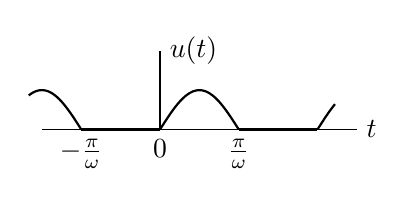
\begin{tikzpicture}
\draw(-1.5,0)--(2.5,0)node[right]{$t$};
\draw(0,0)--(0,1)node[right]{$u(t)$};
%
\draw[thick,domain=-300:-180,smooth] plot ({\x/180},{0.5*sin(\x)});
\draw[thick,domain=0:180,smooth] plot ({\x/180},{0.5*sin(\x)});
\draw[thick,domain=360:400,smooth] plot ({\x/180},{0.5*sin(\x)});
\draw[thick](-1,0)--(0,0)(1,0)--(2,0);
\draw(-1,0)node[below]{$-\frac{\pi}{\omega}$};
\draw(0,0)node[below]{$0$};
\draw(1,0)node[below]{$\frac{\pi}{\omega}$};
\end{tikzpicture}
\caption{نصف لہر سمت کار (مثال \حوالہ{مثال_فوریئر_نصف_لہر_سمت_کار})}
\label{شکل_مثال_فوریئر_نصف_لہر_سمت_کار}
\end{figure}
%
 \begin{align*}
u(t)=
\begin{cases}
0&-\frac{T}{2}<t<0\\
E\sin \omega t&\phantom{-}0<t<\frac{T}{2}
\end{cases}
\end{align*}
حل:یہاں \عددی{T=\tfrac{2\pi}{\omega}} کے برابر ہے۔یوں مساوات \حوالہ{مساوات_فوریئر_عمومی_یولر}-الف سے
\begin{align*}
a_0&=\frac{\omega}{2\pi}\int_{0}^{\frac{\pi}{\omega}} E\sin \omega t\, \dif t=\frac{E}{\pi}
\end{align*}
ملتا ہے جبکہ مساوات \حوالہ{مساوات_فوریئر_عمومی_یولر}-ب میں ضمیمہ \حوالہ{ضمیمہ_مفید_معلومات} کی مساوات \حوالہ{مساوات_ضمیمہ_مفید_گیارہ} استعمال کرتے ہوئے
\begin{align*}
a_n=\frac{\omega}{\pi}\int_0^{\frac{\pi}{\omega}} E\sin \omega t\,\cos n\omega t\,\dif t=\frac{\omega E}{2\pi}\int_0^{\frac{\pi}{\omega}} [\sin(1+n)\omega t+\sin(1-n)\omega t]\dif t
\end{align*}
سے \عددی{n=1} کے لئے صفر جبکہ \عددی{n=2,3,\cdots} کے لئے
\begin{align*}
a_n&=\frac{\omega E}{2\pi}\big[-\frac{\cos(1+n)\omega t}{(1+n)\omega}-\frac{\cos(1-n)\omega t}{(1-n)\omega}\big]_{0}^{\frac{\pi}{\omega}}\\
&=\frac{E}{2\pi}\big(\frac{-\cos(1+n)\pi+1}{1+n}+\frac{-\cos(1-n)\pi+1}{1-n}\big)
\end{align*}
ملتی ہے جو طاق \عددی{n} کے لئے صفر اور جفت \عددی{n} کے لئے 
\begin{align*}
a_n=\frac{E}{2\pi}\big(\frac{2}{1+n}+\frac{2}{1-n}\big)=-\frac{2E}{(n-1)(n+1)\pi}\quad \quad (n=2,4,\cdots)
\end{align*}
دیتی ہے۔اسی طرح مساوات \حوالہ{مساوات_فوریئر_عمومی_یولر}-پ سے \عددی{b_1=\tfrac{E}{2}} جبکہ \عددی{n=2,3,\cdots} کے لئے  \عددی{b_n=0} ملتے ہیں۔اس طرح فوریئر تسلسل درج ذیل ہو گی۔
\begin{align*}
u(t)=\frac{E}{\pi}+\frac{E}{2}\sin \omega t-\frac{2E}{\pi}\big(\frac{1}{1\cdot 3}\cos 2\omega t+\frac{1}{3\cdot 5}\cos 4\omega t+\cdots\big)
\end{align*}
\انتہا{مثال}
%========================

\حصہء{سوالات}

%=======================
\ابتدا{سوال}\quad
اس بات کی تصدیق کریں کہ مساوات \حوالہ{مساوات_فوریئر_عمومی} میں تمام ارکان کا دوری عرصہ \عددی{T} ہے۔
\انتہا{سوال}
%======================
\ابتدا{سوال}\quad اس بات کی تصدیق کریں کہ مساوات \حوالہ{مساوات_فوریئر_عمومی_یولر} میں \عددی{T} کے برابر کسی بھی وقفے پر تکمل حاصل کیا جا سکتا ہے۔
\انتہا{سوال}
%======================
\ابتدا{سوال}\quad
مثال \حوالہ{مثال_فوریئر_نصف_لہر_سمت_کار} کی چکور تفاعل کی تسلسل کو سوال \حوالہ{سوال_فوریئر_تسلسل_دریافت_کریں_الف} کی تسلسل  سے سیدھ و سیدھ بذریعہ تبدیلی متغیر حاصل کریں۔ 
\انتہا{سوال}
%======================
\ابتدا{سوال}\quad
نصف لہر سمت کار کو \عددی{v=E\cos  t} داخلی دباو مہیا کی جاتی ہے۔خارجی دباو کی فوریئر تسلسل حاصل کریں۔\\
جواب:\quad
$\tfrac{1}{\pi}+\tfrac{1}{2}\cos t+\tfrac{2}{\pi}(\tfrac{1}{3}\cos 2t-\tfrac{1}{15}\cos 4t+\tfrac{1}{35}\cos 6t-+\cdots)$
\انتہا{سوال}
%========================
سوال \حوالہ{سوال_فوریئر_عمومی_دوری_عرصہ_الف} تا سوال \حوالہ{سوال_فوریئر_عمومی_دوری_عرصہ_ب} میں تفاعل \عددی{f(t)} کا دوری عرصہ \عددی{T} ہے۔اس کی فوریئر تسلسل دریافت کریں۔تفاعل \عددی{f(t)} اور اس کی تسلسل کے اولین تین جزوی مجموعوں کے خط کھینچیں۔آپ دیکھیں گے کہ تسلسل کی زیادہ ارکان استعمال کرنے سے اصل تفاعل سے زیادہ قریبی مشابہت رکھنے والا خط حاصل ہوتا ہے۔

%=====================
\ابتدا{سوال}\شناخت{سوال_فوریئر_عمومی_دوری_عرصہ_الف}\quad
$f(t)=-1\quad (-1<t<0), \quad f(t)=1\quad (0<t<1),\quad T=2$\\
جواب:\quad
$\tfrac{4}{\pi}(\sin \pi t+\tfrac{1}{3}\sin 3\pi t+\tfrac{1}{5}\sin 5\pi t+\cdots)$
\انتہا{سوال}
%=========================
\ابتدا{سوال}\quad
$f(t)=1\quad (-1<t<2), \quad f(t)=0\quad (2<t<3),\quad T=4$\\
جواب:\quad
$\tfrac{3}{4}+\tfrac{1}{\pi}(\cos \tfrac{\pi t}{2}+\sin \tfrac{\pi t}{2}-\sin \pi t-\tfrac{1}{3}\cos \tfrac{3\pi t}{2}+\tfrac{1}{3}\sin \tfrac{3\pi t}{2}\cdots)$
\انتہا{سوال}
%=========================
\ابتدا{سوال}\شناخت{سوال_فوریئر_درکار_چھلانگ_پ}\quad
$f(t)=1\quad (-1<t<1),\quad T=4$\\
جواب:\quad
$\tfrac{1}{2}+\tfrac{2}{\pi}(\cos \tfrac{\pi t}{2}-\tfrac{1}{3}\cos \tfrac{3\pi t}{2}+\tfrac{1}{5}\cos \tfrac{5\pi t}{2}\cdots)$
\انتہا{سوال}
%=========================
\ابتدا{سوال}\quad
$f(t)=t\quad (-1<t<1),\quad T=2$\\
جواب:\quad
$\tfrac{1}{\pi}(2\sin \pi t-\sin 2\pi t+\tfrac{2}{3}\sin 3\pi t-\tfrac{1}{2}\sin 4\pi t\cdots)$
\انتہا{سوال}
%=========================
\ابتدا{سوال}\quad
$f(t)=t^2\quad (-1<t<1),\quad T=2$\\
جواب:\quad
$\tfrac{1}{3}+\tfrac{1}{\pi^2}(-4\cos \pi t+\cos 2\pi t-\tfrac{1}{9}\cos 3\pi t+\tfrac{1}{4}\cos 4\pi t\cdots)$
\انتہا{سوال}
%=========================
\ابتدا{سوال}\شناخت{سوال_فوریئر_درکار_چھلانگ_ت}\quad
$f(t)=-t\quad (-1<t<0),\quad f(t)=t\quad (0<t<1)\quad T=2$\\
جواب:\quad
$\tfrac{1}{2}-\tfrac{4}{\pi^2}(\cos \pi t+\tfrac{1}{9}\cos 3\pi t+\tfrac{1}{25}\cos 5\pi t\cdots)$
\انتہا{سوال}
%=========================
\ابتدا{سوال}\شناخت{سوال_فوریئر_مکمل_لہر_سمت_کار_عمومی}\quad مکمل لہر سمت کار\quad 
$f(t)=\sin \pi t\quad (0<t<1),\quad T=1$\\
جواب:\quad
$\tfrac{2}{\pi}-\tfrac{4}{\pi}(\tfrac{1}{3}\cos 2\pi t+\tfrac{1}{15}\cos 4\pi t+\tfrac{1}{35}\cos 6\pi t\cdots)$
\انتہا{سوال}
%=========================
\ابتدا{سوال}\شناخت{سوال_فوریئر_درکار_چھلانگ_ٹ}\quad
$f(t)=-1\quad (-1<t<0),\quad f(t)=t\quad (0<t<1)\quad T=2$\\
جواب:\quad
$-\tfrac{1}{4}-\tfrac{2}{\pi^2}\cos \pi t+\tfrac{3}{\pi}\sin \pi t=\tfrac{1}{2\pi}\sin 2\pi t-\tfrac{2}{9\pi^2}\cos 3\pi t\cdots$
\انتہا{سوال}
%=========================
\ابتدا{سوال}\quad
$f(t)=1\quad (0<t<1),\quad f(t)=2\quad (1<t<2)\quad T=3$\\
جواب:\quad
$1-\tfrac{3\sqrt{3}}{2\pi}\cos \tfrac{2\pi t}{3}+\tfrac{3}{2\pi}\sin \tfrac{2\pi t}{3}\cdots$
\انتہا{سوال}
%=========================
\ابتدا{سوال}\شناخت{سوال_فوریئر_درکار_چھلانگ_ث}\quad
$f(t)=-t\quad (-1<t<0),\quad f(t)=2t\quad (0<t<1)\quad T=2$\\
جواب:\quad
$\tfrac{3}{4}-\tfrac{6}{\pi^2}\cos \pi t+\tfrac{1}{\pi}\sin \pi t-\tfrac{1}{2\pi}\sin 2\pi t-\tfrac{2}{3\pi^2}\cos 3\pi t\cdots$
\انتہا{سوال}
%=========================
\ابتدا{سوال}\شناخت{سوال_فوریئر_عمومی_دوری_عرصہ_ب}\quad
$f(t)=\cos(\pi t)\quad (-1<t<1),\quad T=2$\\
جواب:\quad
$\cos \pi t$
\انتہا{سوال}
%=========================
\ابتدا{سوال}\quad
مکمل لہر سمت کار کی فوریئر تسلسل سوال \حوالہ{سوال_فوریئر_مکمل_لہر_سمت_کار_عمومی} میں حاصل کی گئی۔سوال \حوالہ{سوال_فوریئر_تسلسل_دریافت_کریں_ٹ} میں حاصل کی گئی تسلسل میں متغیر تبدیل کرتے ہوئے یہی جواب دوبارہ حاصل کریں۔
\انتہا{سوال}
%==========================

\حصہ{جفت اور طاق تفاعل}
جفت تفاعل کی صورت میں \عددی{b_n=0} جبکہ طاق تفاعل کی صورت میں \عددی{a_n=0} حاصل ہوتا ہے۔یوں یہ جاننے سے کہ آیا تفاعل جفت یا طاق ہے، عددی سر دریافت کرنے کا کام نسبتاً کم ہو گا۔

تمام \عددی{x} کے لئے درج ذیل خاصیت والے تفاعل \عددیء{y=g(x)} کو \اصطلاح{جفت}\فرہنگ{جفت}\حاشیہب{even}\فرہنگ{even} تفاعل کہتے ہیں۔
\begin{align}\label{مساوات_فوریئر_جفت_تعریف}
g(-x)=g(x)
\end{align}
ایسا تفاعل \عددی{y} محور کی دونوں اطراف تشاکلی (شکل \حوالہ{شکل_فوریئر_جفت_طاق}-الف) ہو گا۔اس کے برعکس تفاعل \عددی{y=h(x)} جس کی خاصیت درج ذیل ہو \اصطلاح{طاق}\فرہنگ{طاق}\حاشیہب{odd}\فرہنگ{odd} تفاعل کہلاتا ہے (شکل \حوالہ{شکل_فوریئر_جفت_طاق}-ب)۔
\begin{align}\label{مساوات_فوریئر_طاق_تعریف}
h(-x)=-h(x)
\end{align}
%
\begin{figure}
\centering
\begin{subfigure}{0.5\textwidth}
\centering
\begin{tikzpicture}
\draw(-2,0)--(2,0)node[right]{$x$};
\draw(0,-0.5)--(0,1.5)node[left]{$y$};
\draw(0,0) to [out=180,in=0]++(-0.5,-0.25) to [out=180,in=-45] (-2,1);
\draw(0,0)node[ocirc]{} to [out=0,in=180]++(0.5,-0.25) to [out=0,in=-135] (2,1);
\end{tikzpicture}
\caption*{(الف) جفت تفاعل}
\end{subfigure}%
\begin{subfigure}{0.5\textwidth}
\centering
\begin{tikzpicture}
\draw(-2,0)--(2,0)node[right]{$x$};
\draw(0,-1.5)--(0,1.5)node[left]{$y$};
\draw(0,0) to [out=180,in=0]++(-0.5,0.25) to [out=180,in=45] (-2,-1);
\draw(0,0)node[ocirc]{} to [out=0,in=180]++(0.5,-0.25) to [out=0,in=-135] (2,1);
\end{tikzpicture}
\caption*{(ب) طاق تفاعل}
\end{subfigure}%
\caption{جفت اور طاق تفاعل}
\label{شکل_فوریئر_جفت_طاق}
\end{figure}

جفت تفاعل \عددی{g(x)} کی صورت میں \عددی{y} محور کی دائیں ہاتھ ترسیم کے نیچے رقبہ، محور کی بائیں ہاتھ ترسیم کے نیچے رقبہ کے  برابر ہے (شکل \حوالہ{شکل_فوریئر_جفت_طاق}-الف) لہٰذا \عددی{g(x)} کے لئے درج ذیل لکھا جا سکتا ہے۔
\begin{align}\label{مساوات_فوریئر_جفت_تفاعل_تکمل}
\int_{-\frac{T}{2}}^{\frac{T}{2}}g(x)\,\dif x=\int_{-\frac{T}{2}}^{0}g(x)\,\dif x+\int_{0}^{\frac{T}{2}}g(x)\,\dif x=2\int_{0}^{\frac{T}{2}}g(x),\dif x\quad \quad (\text{\RL{جفت $g$}})
\end{align}
طاق تفاعل \عددی{h(x)} کی صورت میں \عددی{y} محور کی دائیں ہاتھ ترسیم کے نیچے رقبہ، محور کی بائیں ہاتھ ترسیم کے نیچے رقبہ ضرب منفی اکائی کے برابر ہے (شکل \حوالہ{شکل_فوریئر_جفت_طاق}-ب) لہٰذا \عددی{h(x)} کے لئے درج ذیل لکھا جا سکتا ہے۔
\begin{align}\label{مساوات_فوریئر_طاق_تفاعل_تکمل}
\int_{-\frac{T}{2}}^{\frac{T}{2}}h(x)\,\dif x==\int_{-\frac{T}{2}}^{0}h(x)\,\dif x+\int_{0}^{\frac{T}{2}}h(x)\,\dif x=0\quad \quad (\text{\RL{طاق $h$}})
\end{align}

جفت تفاعل \عددی{g(x)} اور طاق تفاعل \عددی{h(x)} کی حاصل ضرب \عددی{q=gh} کے لئے
\begin{align*}
q(-x)=g(-x)h(-x)=g(x)[-h(x)]=-g(x)h(x)=-q(x)
\end{align*}
لکھا جا سکتا ہے لہٰذا  \عددی{q=gh} طاق تفاعل ہو گا۔یوں اگر \عددی{f(t)} جفت تفاعل ہو تب مساوات \حوالہ{مساوات_فوریئر_عمومی_یولر}-پ میں متکمل \عددی{f(t)\sin \tfrac{2n\pi t}{T}} طاق ہو گا لہٰذا \عددی{b_n=0} ہو گا۔اسی طرح اگر \عددی{f(t)} طاق ہو تب مساوات \حوالہ{مساوات_فوریئر_عمومی_یولر}-ب میں \عددی{f\cos \tfrac{2n\pi t}{T}} طاق ہو گا لہٰذا \عددی{a_n=0} ہو گا۔ان نتائج سے درج ذیل مسئلہ اخذ ہوتا ہے۔

%===============
\ابتدا{مسئلہ}\شناخت{مسئلہ_فوریئر_جفت_طاق_تسلسل}\quad جفت اور طاق تفاعل کی فوریئر تسلسل\\ 
دوری عرصہ \عددی{T} کی جفت تفاعل \عددی{f(t)} کی فوریئر تسلسل، \اصطلاح{فوریئر کوسائن تسلسل}\فرہنگ{فوریئر!کوسائن تسلسل}\حاشیہب{Fourier cosine series}\فرہنگ{Fourier!cosine series}
\begin{align}\label{مساوات_فوریئر_جفت_فوریئر_تسلسل}
f(t)=a_0+\sum_{n=1}^{\infty} a_n\cos \frac{2n\pi}{T}t\quad \quad \quad (\text{\RL{جفت $f$}})
\end{align}
 ہو گی جس کے عددی سر درج ذیل ہوں گے۔
\begin{align}\label{مساوات_فوریئر_جفت_تسلسل_عددی_سر}
a_0=\frac{2}{T}\int_{0}^{\frac{T}{2}}f(t)\,\dif t, \quad a_n=\frac{4}{T}\int_{0}^{\frac{T}{2}}f(t)\cos \frac{2n\pi}{T}t\,\dif t,\quad n=1,2,\cdots
\end{align}
 
دوری عرصہ \عددی{T} کی طاق تفاعل \عددی{f(t)} کی فوریئر تسلسل، \اصطلاح{فوریئر سائن تسلسل}\فرہنگ{فوریئر!سائن تسلسل}\حاشیہب{Fourier sine series}\فرہنگ{Fourier!sine series}
\begin{align}\label{مساوات_فوریئر_طاق_فوریئر_تسلسل}
f(t)=\sum_{n=1}^{\infty} b_n\sin \frac{2n\pi}{T}t\quad \quad \quad (\text{\RL{طاق $f$}})
\end{align}
 ہو گی جس کے عددی سر درج ذیل ہوں گے۔
\begin{align}\label{مساوات_فوریئر_طاق_تسلسل_عددی_سر}
b_n=\frac{4}{T}\int_{0}^{\frac{T}{2}}f(t)\sin \frac{2n\pi}{T}t\,\dif t,\quad n=1,2,\cdots
\end{align}
\انتہا{مسئلہ}
%==================

اس مسئلہ کے تحت دوری عرصہ \عددی{2\pi} کی جفت تفاعل \عددی{f(x)} کی فوریئر تسلسل درج ذیل فوریئر کوسائن تسلسل 
\begin{align}
f(x)=a_0+a_1\cos x+a_2\cos 2x+a_3\cos 3x+\cdots\quad \quad \quad (\text{\RL{جفت $f$}})
\end{align} 
ہو گی جس کے فوریئر عددی سر 
\begin{align}
a_0=\frac{1}{\pi}\int_0^{\pi}f(x)\,\dif x,\quad a_n=\frac{2}{\pi}\int_0^{\pi} f(x)\cos nx\,\dif x,\quad n=1,2,\cdots
\end{align}
ہوں گے۔اسی طرح دوری عرصہ \عددی{2\pi} والی تفاعل \عددی{f(x)} کی فوریئر سائن تسلسل 
\begin{align}
f(x)=b_1\sin x+b_2\sin 2x+b_3\sin 3x+\cdots\quad \quad \quad (\text{\RL{طاق $f$}})
\end{align}
پائی جائے گی جس کے عددی سر درج ذیل ہوں گے۔
\begin{align}
b_n=\frac{2}{\pi}\int_0^{\pi}f(x)\sin nx\,\dif x,\quad n=1,2,\cdots
\end{align}

مثال \حوالہ{مثال_فوریئر_عمومی_چکور} میں دی گئی چکور تفاعل جفت ہے لہٰذا اس کی فوریئر کوسائن تسلسل پائی گئی۔ 

مزید آسانی درج ذیل مسئلہ سے حاصل ہوتی ہے۔

%===================
\ابتدا{مسئلہ}\شناخت{مسئلہ_فوریئر_مجموعہ_تفاعل_عددی_سر}\quad (تفاعل کا مجموعہ)
مجموعہ تفاعل \عددی{f_1+f_2} کی فوریئر عددی سر،  تفاعل \عددی{f_1}  اور تفاعل \عددی{f_2} کی مطابقتی فوریئر عددی سر کا مجموعہ ہو گا۔ 
\انتہا{مسئلہ}
%======================

کسی بھی تفاعل \عددی{f(x)} کو درج ذیل لکھا جا سکتا ہے
\begin{align}
f(x)=\frac{1}{2}[f(x)+f(-x)]+\frac{1}{2}[f(x)-f(-x)]=g(x)+h(x)
\end{align}
جہاں
\begin{gather}
\begin{aligned}\label{مساوات_فوریئر_جفت_طاق_مجموعہ_کوئی_تفاعل}
g(x)&=\tfrac{1}{2}[f(x)+f(-x)]\\
h(x)&=\tfrac{1}{2}[f(x)-f(-x)]
\end{aligned}
\end{gather}
 ہیں۔درج ذیل سے  ثابت ہوتا ہے کہ \عددی{g(x)} جفت اور \عددی{h(x)} طاق ہیں (مساوات \حوالہ{مساوات_فوریئر_جفت_تعریف} اور مساوات \حوالہ{مساوات_فوریئر_طاق_تعریف})۔
\begin{align*}
g(-x)&=\frac{1}{2}[f(-x)+f(x)]=\frac{1}{2}[f(x)+f(-x)]=g(x)\\
h(-x&)=\frac{1}{2}[f(-x)-f(x)]=-\frac{1}{2}[f(x)-f(-x)]=-h(x)
\end{align*}
یوں کسی بھی تفاعل \عددی{f(x)} کو جفت تفاعل \عددی{g(h)} اور طاق تفاعل \عددی{h(x)} کا مجموعہ لکھا جا سکتا ہے جنہیں مساوات \حوالہ{مساوات_فوریئر_جفت_طاق_مجموعہ_کوئی_تفاعل} سے حاصل کیا جاتا ہے۔
%==========================
\ابتدا{مثال}\شناخت{مثال_فوریئر_مستطیل_دھڑکن}\quad مستطیل دھڑکن\\
مستطیل \اصطلاح{دھڑکن}\فرہنگ{دھڑکن}\حاشیہب{pulse}\فرہنگ{pulse} \عددی{f^*(x)} کو شکل \حوالہ{شکل_مثال_فوریئر_مستطیل_دھڑکن} میں دکھایا گیا ہے۔آپ دیکھ سکتے ہیں کہ سوال \حوالہ{سوال_فوریئر_تسلسل_دریافت_کریں_پ}  میں دکھائی گئی تفاعل \عددی{f(x)} کے ساتھ \عددی{1} جمع کرنے سے موجودہ تفاعل \عددی{f^*(x)} حاصل ہو گی۔یوں  سوال \حوالہ{سوال_فوریئر_تسلسل_دریافت_کریں_پ} میں حاصل کیے گئے فوریئر تسلسل سے \عددی{f^*(x)} کی فوریئر تسلسل سیدھ و سیدھ لکھتے ہیں۔ 
\begin{align*}
1+\tfrac{4}{\pi}(\sin x+\tfrac{1}{3}\sin 3x+\tfrac{1}{5}\sin 5x+\cdots)
\end{align*}

\begin{figure}
\centering
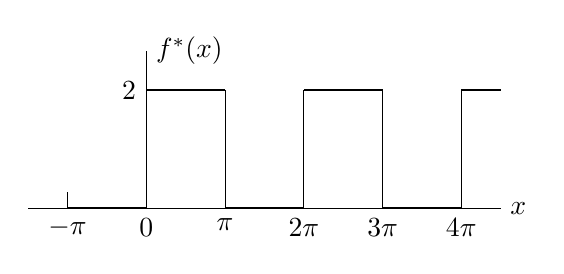
\begin{tikzpicture}
\draw(-1.5,0)--(4.5,0)node[right]{$x$};
\draw(0,0)--(0,2)node[right]{$f^*(x)$};
%
\draw[thick](-1,0)node[below]{$-\pi$}--(0,0)node[below]{$0$}(1,0)node[below]{$\pi$}--(2,0)node[below]{$2\pi$}(3,0)node[below]{$3\pi$}--(4,0)node[below]{$4\pi$};
\draw[thick](0,1.5)node[left]{$2$}--++(1,0)++(1,0)--++(1,0)++(1,0)--++(0.5,0);
\draw(1,0)--++(0,1.5);
\draw(2,0)--++(0,1.5);
\draw(3,0)--++(0,1.5);
\draw(4,0)--++(0,1.5);
%
\draw(-1,0)--++(0,0.2);
\end{tikzpicture}
\caption{مستطیل دھڑکن (مثال \حوالہ{مثال_فوریئر_مستطیل_دھڑکن})}
\label{شکل_مثال_فوریئر_مستطیل_دھڑکن}
\end{figure}
\انتہا{مثال}
%========================
\ابتدا{مثال}\شناخت{مثال_فوریئر_دندان_موج}\quad دندان موج\\
\اصطلاح{دندان موج}\فرہنگ{دندان موج}\فرہنگ{موج!دندان}\حاشیہب{saw tooth wave}\فرہنگ{saw tooth wave}
\begin{align*}
f(x)=x+\pi,\quad (-\pi<x<\pi); \quad f(x+2\pi)=f(x)
\end{align*}
 کو شکل \حوالہ{شکل_مثال_فوریئر_دندان_موج}-الف میں دکھایا گیا ہے۔اس کی فوریئر تسلسل دریافت کریں۔
\begin{figure}
\centering
\begin{subfigure}{0.5\textwidth}
\centering
\begin{tikzpicture}
\draw(-2,0)--(2,0)node[below]{$x$};
\draw(0,0)node[ocirc]{}--(0,1.5)node[right]{$f(x)$};
%
\draw[thick](-1.5,1)--++(45:-0.4);
\draw[thick](1.5,0)--++(45:0.4);
\draw(1.5,0)--++(0,1);
\foreach \x in {-1.5,-0.5,0.5} {\draw[thick](\x,0)--++(1,1);\draw(\x,0)--++(0,1);}
\draw(-0.5,0)node[below]{$-\pi$};
\draw(0.5,0)node[below]{$\pi$};
\end{tikzpicture}
\caption*{(الف) دی گئی دندان موج $f(x)$}
\end{subfigure}
\begin{subfigure}{1\textwidth}
\centering
\begin{tikzpicture}
\pgfmathsetmacro{\k}{0.5}
%grid
%\draw[thick](-4,0) grid (4,3);
%\draw[thin,gray,step=0.1] (-4,0) grid (4,3);
%axis
\draw(-4.5,0)--(5,0)node[right]{$x$};
\draw(0,0)node[below]{$0$}--(0,3);
%
\draw(-4,1)--(-4,0)--(4,3.142)node[right]{\RL{دندان موج}}--(4,2);
\draw[thin,domain=-180:180,smooth] plot ({4/180*\x},{\k*(3.142+2*sin(\x))});
\draw[dashed,domain=-180:180,smooth] plot ({4/180*\x},{\k*(3.142+2*sin(\x)-sin(2*\x))});
\draw[thick,domain=-180:180,smooth] plot ({4/180*\x},{\k*(3.142+2*sin(\x)-sin(2*\x)+2/3*sin(3*\x))});
%
\draw(-4,0)node[below]{$-\pi$}--++(0,0.2);
\draw(4,0)node[below]{$\pi$}--++(0,0.2);
%
\draw[stealth-](1.2,2.4) to [out=90,in=0]++(-0.25,0.25)node[left]{$S_1$};
\draw[stealth-](2.3,2.8) to [out=90,in=0]++(-0.25,0.25)node[left]{$S_2$};
\draw[stealth-](3,3) to [out=90,in=0]++(-0.25,0.25)node[left]{$S_3$};
\end{tikzpicture}
\caption*{(ب) جزوی مجموعے}
\end{subfigure}
\caption{دندان موج اور اس کا فوریئر تسلسل (مثال \حوالہ{مثال_فوریئر_دندان_موج})}
\label{شکل_مثال_فوریئر_دندان_موج}
\end{figure}
حل:دندان موج کی تفاعل کو
\begin{align*}
f=f_1+f_2;\quad f_1=x,\quad f_2=\pi
\end{align*}
لکھا جا سکتا ہے۔\عددی{f_2} کی فوریئر عددی سر صفر کے برابر ہیں ماسوائے \عددی{a_0} کے جو \عددی{\pi} کے برابر ہے۔یوں مسئلہ \حوالہ{مسئلہ_فوریئر_مجموعہ_تفاعل_عددی_سر} کے تحت دندان موج کے عددی سر \عددی{a_n}، \عددی{b_n} تفاعل \عددی{f_1} کے عددی سر ہوں گے جبکہ اس کا \عددی{a_0=\pi} ہو گا (\عددی{f_1} طاق ہے لہٰذا اس کا اپنا \عددی{a_0=0} ہے)۔یوں
\begin{align*}
b_n=\frac{2}{\pi}\int_0^{\pi} f_1(x)\sin nx\,\dif x=\frac{2}{\pi}\int_0^{\pi} x\sin nx\,\dif x
\end{align*}
کا تکمل بالحصص لینے سے
\begin{align*}
b_n=\frac{2}{\pi}\big[\left. \frac{-x\cos nx}{n}\right|_0^{\pi}+\frac{1}{n}\int_0^{\pi} \cos nx\,\dif x\big]=-\frac{2}{n}\cos n\pi
\end{align*}
ملتا ہے جس سے \عددی{b_1=2}، \عددی{b_2=-1}، \عددی{b_3=\tfrac{2}{3}}، \عددی{b_4=-\tfrac{1}{2}}، \نقطے حاصل ہوتے ہیں لہٰذا دندان موج کی فوریئر تسلسل درج ذیل ہو گی (شکل \حوالہ{شکل_مثال_فوریئر_دندان_موج}-ب)۔
\begin{align*}
f(x)=\pi+2\big(\sin x-\frac{1}{2}\sin 2x+\frac{1}{3}\sin 3x-+\cdots\big)
\end{align*}

\انتہا{مثال}
%===========================

\حصہء{سوالات}

%=================
\ابتدا{سوال}\quad کیا درج ذیل تفاعل جفت، طاق یا ان میں سے دونوں نہیں (نہ طاق اور نہ ہی جفت) ہیں؟\\
\begin{align*}
e^x,\, e^{x^2},\, \sin nx,\,x\sin nx,\, \frac{\cos x}{x},\, \ln x,\, \sin x^2,\, \sin^2 x
\end{align*}
جوابات:بائیں سے  \عددی{4}، \عددی{6} طاق، \عددی{3}، \عددی{9} دونوں نہیں اور باقی تمام جفت ہیں۔
\انتہا{سوال}
%======================
سوال \حوالہ{سوال_فوریئر_جفت_طاق_معلوم_الف} تا سوال \حوالہ{سوال_فوریئر_جفت_طاق_معلوم_ب} میں دوری تفاعل \عددی{f(x)} کا دوری عرصہ \عددی{2\pi} ہے۔کیا تفاعل جفت، طاق یا دونوں نہیں ہیں۔

%==============
\ابتدا{سوال}\شناخت{سوال_فوریئر_جفت_طاق_معلوم_الف}\quad
$f(x)=\abs{x},\quad (-\pi<x<\pi)$\\
جواب:\quad جفت
\انتہا{سوال}
%====================
\ابتدا{سوال}\شناخت{سوال_فوریئر_جفت_طاق_معلوم_الف_بعد_ب}\quad
$f(x)=x,\quad (-\pi<x<\pi)$\\
جواب:\quad طاق
\انتہا{سوال}
%====================
\ابتدا{سوال}\شناخت{سوال_فوریئر_جفت_طاق_معلوم_الف_بعد_پ}\quad
$f(x)=x^2,\quad (-\pi<x<\pi)$\\
جواب:\quad جفت
\انتہا{سوال}
%====================
\ابتدا{سوال}\quad
$f(x)=x^3,\quad (-\pi<x<\pi)$\\
جواب:\quad طاق
\انتہا{سوال}
%====================
\ابتدا{سوال}\شناخت{سوال_فوریئر_جفت_طاق_معلوم_الف_بعد_ت}\quad
$f(x)=e^x,\quad (-\pi<x<\pi)$\\
جواب:\quad نہ طاق اور نہ ہی جفت
\انتہا{سوال}
%====================
\ابتدا{سوال}\quad
$f(x)=e^{\abs{x}},\quad (-\pi<x<\pi)$\\
جواب:\quad جفت
\انتہا{سوال}
%====================
\ابتدا{سوال}
\begin{align*}
f(x)=
\begin{cases}
-1&-\pi<x<0\\
\phantom{-}1& \phantom{-} 0<x<\pi
\end{cases}
\end{align*}
جواب:\quad طاق
\انتہا{سوال}
%=====================
\ابتدا{سوال}\شناخت{سوال_فوریئر_جفت_طاق_معلوم_ب}\quad 
$f(x)=1,\quad (-\frac{\pi}{2}<x<\frac{\pi}{2})$
جواب:\quad جفت
\انتہا{سوال}
%=====================
\ابتدا{سوال}\quad ایسا تفاعل دریافت کریں جو جفت بھی ہو اور طاق بھی۔\\
جواب:\quad \عددی{f(x)=0}
\انتہا{سوال}
%=====================
\ابتدا{سوال}\quad مساوات \حوالہ{مساوات_فوریئر_جفت_تفاعل_تکمل} اور مساوات \حوالہ{مساوات_فوریئر_طاق_تفاعل_تکمل} ثابت کریں۔
\انتہا{سوال}
%====================
\ابتدا{سوال}\quad مسئلہ \حوالہ{مسئلہ_فوریئر_مجموعہ_تفاعل_عددی_سر} کو ثابت کریں۔
\انتہا{سوال}
%========================
سوال \حوالہ{سوال_فوریئر_جفت_طاق_کا_مجموعہ_الف} تا سوال \حوالہ{سوال_فوریئر_جفت_طاق_کا_مجموعہ_ب} میں دیے گئے تفاعل کو  ایک عدد جفت تفاعل اور ایک عدد طاق تفاعل کا مجموعہ لکھیں۔

%==========================
\ابتدا{سوال}\شناخت{سوال_فوریئر_جفت_طاق_کا_مجموعہ_الف}\quad
$\tfrac{1}{1-x}$\\
جواب:\quad
$\tfrac{1}{1-x^2}+\tfrac{x}{1-x^2}$
\انتہا{سوال}
%===============================
\ابتدا{سوال}
$\tfrac{1}{1-x^2}$\\
جواب:\quad
$\frac{1+x^2}{(1-x^2)^2}+\frac{2x}{(1-x^2)^2}$
\انتہا{سوال}
%=============================
\ابتدا{سوال}\quad 
$e^x$\\
جواب:\quad
$\cosh x+\sinh x$
\انتہا{سوال}
%========================
\ابتدا{سوال}\شناخت{سوال_فوریئر_جفت_طاق_کا_مجموعہ_ب}\quad
$\cos x$\\
جواب:\quad جفت تفاعل یا طاق تفاعل جوں کا توں لکھا جائے گا۔\quad
$\cos x$

\انتہا{سوال}
%============================
\ابتدا{سوال}\quad 
ثابت کریں کہ دو عدد جفت تفاعل کا مجموعہ جفت تفاعل ہو گا۔
\انتہا{سوال}
%=======================
\ابتدا{سوال}\quad 
ثابت کریں کہ دو عدد جفت تفاعل کا حاصل ضرب جفت تفاعل ہو گا۔
\انتہا{سوال}
%=======================
\ابتدا{سوال}\quad 
ثابت کریں کہ دو عدد طاق تفاعل کا مجموعہ طاق تفاعل ہو گا۔
\انتہا{سوال}
%=======================
\ابتدا{سوال}\quad 
ثابت کریں کہ دو عدد طاق تفاعل کا حاصل ضرب جفت تفاعل ہو گا۔
\انتہا{سوال}
%=======================
\ابتدا{سوال}\quad
ثابت کریں کہ جفت \عددی{f(x)} کی صورت میں \عددی{\abs{f(x)}+f^2(x)} جفت ہو گا۔
\انتہا{سوال}
%======================
\ابتدا{سوال}\quad
ثابت کریں کہ طاق \عددی{f(x)} کی صورت میں \عددی{\abs{f(x)}+f^2(x)} اور \عددی{f^3(x)} جفت ہوں گے۔
\انتہا{سوال}
%======================
سوال \حوالہ{سوال_فوریئر_تسلسل_درکار_الف} تا سوال \حوالہ{سوال_فوریئر_تسلسل_درکار_پ} میں دیے گئے تفاعل کا دوری عرصہ \عددی{2\pi} ہے۔ان تفاعل کی فوریئر تسلسل حاصل کریں۔

%=================
\ابتدا{سوال}\شناخت{سوال_فوریئر_تسلسل_درکار_الف}
\begin{align*}
f(x)=
\begin{cases}
\phantom{-}1&-\frac{\pi}{2}<x<\frac{\pi}{2}\\
-1&\phantom{-} \frac{\pi}{2}<x<\frac{3\pi}{2}
\end{cases}
\end{align*}
جواب:\quad
$\tfrac{4}{\pi}(\cos x-\tfrac{1}{3}\cos 3x+\tfrac{1}{5}\cos 5x\cdots)$
\انتہا{سوال}
%=====================
\ابتدا{سوال}
\begin{align*}
f(x)=
\begin{cases}
x&0<x<\pi\\
\pi-x&\pi<x<2\pi
\end{cases}
\end{align*}
جواب:\quad
$-\tfrac{4}{\pi}\cos x+2\sin x-\tfrac{4}{9\pi}\cos 3x+\tfrac{2}{3}\sin 3x-\tfrac{4}{25}\cos 5x+\tfrac{2}{5}\sin 5x\cdots$
\انتہا{سوال}
%=====================
\ابتدا{سوال}
\begin{align*}
f(x)=
\begin{cases}
\phantom{-}x&-\pi<x<0\\
-x&\phantom{-}0<x<\pi
\end{cases}
\end{align*}
جواب:\quad
$-\tfrac{\pi}{2}+\tfrac{4}{\pi}(\cos x+\tfrac{1}{9}\cos 3x+\tfrac{1}{25}\cos 5x\cdots)$
\انتہا{سوال}
%=====================
\ابتدا{سوال}
\begin{align*}
f(x)=
\begin{cases}
\pi+x&-\pi<x<0\\
\pi-x&\phantom{-}0<x<\pi
\end{cases}
\end{align*}
جواب:\quad
$\tfrac{\pi}{2}+\tfrac{4}{\pi}(\cos x+\tfrac{1}{9}\cos 3x+\tfrac{1}{25}\cos 5x\cdots)$
\انتہا{سوال}
%=====================
\ابتدا{سوال}\شناخت{سوال_فوریئر_تسلسل_درکار_ب}\quad
$f(x)=\frac{x^2}{4},\quad (-\pi<x<\pi)$\\
جواب:\quad
$\tfrac{\pi^2}{12}-\cos x+\tfrac{1}{4}\cos 2x-\tfrac{1}{9}\cos 3x+\tfrac{1}{16}\cos 4x-+\cdots$
\انتہا{سوال}
%=====================
\ابتدا{سوال}\شناخت{سوال_فوریئر_تسلسل_درکار_پ}
\begin{align*}
f(x)=
\begin{cases}
x^2&-\pi<x<0\\
x&\phantom{-}0<x<\pi
\end{cases}
\end{align*}
جواب:\quad
$\tfrac{\pi^2}{6}+\tfrac{\pi}{4}-\tfrac{2}{\pi}(\pi+1)\cos x+\tfrac{1}{\pi}(-\pi^2+\pi+4)\sin x+\tfrac{1}{2}\cos 2x\cdots$
\انتہا{سوال}
%=====================
سوال \حوالہ{سوال_فوریئر_تصدیق_درکار_الف} تا سوال \حوالہ{سوال_فوریئر_تصدیق_درکار_ت} میں دی گئی تعلق کو ثابت کریں (مساوات \حوالہ{مساوات_فوریئر_لیبنٹز_تعلق} دیکھیں)۔

%=====================
\ابتدا{سوال}\شناخت{سوال_فوریئر_تصدیق_درکار_الف}\quad(سوال \حوالہ{سوال_فوریئر_تسلسل_درکار_الف} یا سوال \حوالہ{سوال_فوریئر_تسلسل_درکار_ب}  استعمال کریں) \quad 
$1-\tfrac{1}{3}+\tfrac{1}{5}-\tfrac{1}{7}+-\cdots=\tfrac{\pi}{4}$

\انتہا{سوال}
%========================
\ابتدا{سوال}\شناخت{سوال_فوریئر_تصدیق_درکار_ب}\quad(سوال \حوالہ{سوال_فوریئر_تسلسل_درکار_ب} استعمال کریں) \quad
$1+\tfrac{1}{4}+\tfrac{1}{9}+\tfrac{1}{16}+\cdots=\tfrac{\pi^2}{6}$

\انتہا{سوال}
%========================
\ابتدا{سوال}\شناخت{سوال_فوریئر_تصدیق_درکار_پ}\quad(سوال \حوالہ{سوال_فوریئر_تسلسل_درکار_ب} استعمال کریں) \quad 
$1-\tfrac{1}{4}+\tfrac{1}{9}-\tfrac{1}{16}+-\cdots=\tfrac{\pi^2}{12}$

\انتہا{سوال}
%========================
\ابتدا{سوال}\شناخت{سوال_فوریئر_تصدیق_درکار_ت}\quad(سوال \حوالہ{سوال_فوریئر_تصدیق_درکار_ب} اور سوال \حوالہ{سوال_فوریئر_تصدیق_درکار_پ} استعمال کریں) \quad 
$1+\tfrac{1}{3^2}+\tfrac{1}{5^2}+\tfrac{1}{7^2}+\cdots=\tfrac{\pi^2}{8}$

\انتہا{سوال}
%========================

\حصہ{نصف حلقہ اتساع}
کئی انجینئری اور طبیعیاتی مسائل میں ایسے تفاعل \عددی{f(t)} کی فوریئر تسلسل درکار ہو گی جو کسی محدود وقفہ \عددی{0\le t\le l}  پر معین ہو۔ہم وقفہ \عددی{0\le t\le l} کو تکمل کا وقفہ \عددی{0\le t\le \tfrac{T}{2}} لیتے ہوئے مسئلہ \حوالہ{مسئلہ_فوریئر_جفت_طاق_تسلسل} استعمال کرتے ہیں۔یوں \عددی{l=\tfrac{T}{2}} یعنی \عددی{T=2l} چنا گیا ہے۔ مساوات \حوالہ{مساوات_فوریئر_جفت_تسلسل_عددی_سر} استعمال کرتے ہوئے فوریئر کوسائن تسلسل حاصل ہوتی ہے جو \عددی{T=2l} عددی عرصہ کی جفت تفاعل \عددی{f_1(t)}  کو ظاہر کرتی ہے۔وقفہ  \عددی{0\le t\le l} پر \عددی{f_1(t)=f(t)} ہو گا۔اسی لئے \عددی{f_1(t)} کو \عددی{f(t)} کی \اصطلاح{جفت دوری توسیع}\فرہنگ{جفت!دوری توسیع}\حاشیہب{even periodic extension}\فرہنگ{even!periodic extension} کہتے ہیں۔شکل \حوالہ{شکل_فوریئر_دوری_توسیع}-ب میں جفت دوری توسیع دکھائی گئی ہے۔مساوات \حوالہ{مساوات_فوریئر_جفت_فوریئر_تسلسل} اور مساوات \حوالہ{مساوات_فوریئر_جفت_تسلسل_عددی_سر} میں \عددی{T=2l} لیتے ہوئے 
\begin{align}\label{مساوات_فوریئر_نصف_حلقہ_توسیع_جفت}
f(t)=a_0+\sum_{n=1}^{\infty} a_n\cos \frac{n\pi}{l}t\quad \quad \quad (0\le t\le l)
\end{align}
جفت فوریئر تسلسل حاصل ہو گی جس کی عددی سر
\begin{align}\label{مساوات_فوریئر_نصف_حلقہ_توسیع_جفت_عددی_سر}
a_0=\frac{1}{l}\int_{0}^{l}f(t)\,\dif t,\quad a_n=\frac{2}{l}\int_0^l f(t)\cos \frac{n\pi}{l}t\,\dif t,\quad n=1,2,\cdots
\end{align}
ہوں گے۔

ہم مسئلہ  \حوالہ{مسئلہ_فوریئر_جفت_طاق_تسلسل} کی مساوات \حوالہ{مساوات_فوریئر_جفت_تسلسل_عددی_سر} کی جگہ، پہلی کی طرح \عددی{T=2l} لیتے ہوئے، مساوات \حوالہ{مساوات_فوریئر_طاق_تسلسل_عددی_سر}  استعمال کر سکتے ہیں۔ایسا کرنے سے فوریئر سائن تسلسل حاصل ہو گی جو دوری عرصہ \عددی{T=2l} کی دوری تفاعل \عددی{f_2(t)} کو ظاہر کرے گی۔وقفہ \عددی{0\le t\le l} پر \عددی{f_2(t)=f(t)} ہو گا۔\عددی{f_2(t)} کو \عددی{f(t)} کی \اصطلاح{طاق دوری توسیع}\فرہنگ{طاق!دوری توسیع}\حاشیہب{odd periodic extension}\فرہنگ{odd!periodic extension} کہتے ہیں۔شکل \حوالہ{شکل_فوریئر_دوری_توسیع}-پ میں طاق دوری توسیع دکھائی گئی ہے۔مساوات \حوالہ{مساوات_فوریئر_طاق_فوریئر_تسلسل} اور مساوات \حوالہ{مساوات_فوریئر_طاق_تسلسل_عددی_سر} میں \عددی{T=2l} لیتے ہوئے 
\begin{align}\label{مساوات_فوریئر_نصف_حلقہ_توسیع_طاق}
f(t)=\sum_{n=1}^{\infty} b_n\sin \frac{n\pi}{l}t\quad \quad \quad (0\le t\le l)
\end{align}
طاق فوریئر تسلسل حاصل ہو گی جس کی عددی سر
\begin{align}\label{مساوات_فوریئر_نصف_حلقہ_توسیع_طاق_عددی_سر}
b_n=\frac{2}{l}\int_0^l f(t)\sin \frac{n\pi}{l}t\,\dif t,\quad n=1,2,\cdots
\end{align}
ہوں گے۔مساوات \حوالہ{مساوات_فوریئر_نصف_حلقہ_توسیع_جفت_عددی_سر} اور مساوات \حوالہ{مساوات_فوریئر_نصف_حلقہ_توسیع_طاق_عددی_سر} میں دی گئی عددی سر استعمال کرتے ہوئے  مساوات \حوالہ{مساوات_فوریئر_نصف_حلقہ_توسیع_جفت} اور مساوات \حوالہ{مساوات_فوریئر_نصف_حلقہ_توسیع_طاق} کو دی گئی تفاعل \عددی{f(t)} کی \اصطلاح{نصف حلقہ اتساع}\فرہنگ{نصف حلقہ اتساع}\حاشیہب{half range expansion}\فرہنگ{half range expansion} کہتے ہیں۔ 
\begin{figure}
\centering
\begin{subfigure}{0.5\textwidth}
\centering
\begin{tikzpicture}
\draw(0,0)--(1.5,0)node[right]{$t$};
\draw(0,0)--(0,1)node[left]{$f(t)$};
%
\draw[thick,domain=0:1,smooth] plot ({\x},{0.25+(\x-0.25)*(\x-0.25)});
\draw(1,0)node[below]{$l$}--++(0,0.2);
\end{tikzpicture}
\caption*{(الف) دیا گیا تفاعل $f(t)$}
\end{subfigure}
\begin{subfigure}{0.5\textwidth}
\centering
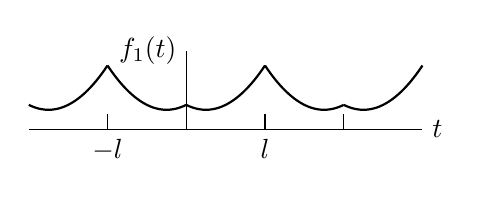
\begin{tikzpicture}
\draw(-2,0)--(3,0)node[right]{$t$};
\draw(0,0)--(0,1)node[left]{$f_1(t)$};
%
\draw[thick,domain=0:1,smooth] plot ({\x},{0.25+(\x-0.25)*(\x-0.25)});
\draw[thick,domain=0:1,smooth] plot ({-\x},{0.25+(\x-0.25)*(\x-0.25)});
\draw[thick,domain=0:1,smooth] plot ({\x-2},{0.25+(\x-0.25)*(\x-0.25)});
\draw[thick,domain=0:1,smooth] plot ({\x+2},{0.25+(\x-0.25)*(\x-0.25)});
\draw[thick,domain=0:1,smooth] plot ({2-\x},{0.25+(\x-0.25)*(\x-0.25)});
\draw(1,0)node[below]{$l$}--++(0,0.2);
\draw(-1,0)node[below]{$-l$}--++(0,0.2);
\draw(2,0)--++(0,0.2);
\end{tikzpicture}
\caption*{(ب) تفاعل $f(t)$ کی جفت دوری توسیع}
\end{subfigure}
\begin{subfigure}{0.5\textwidth}
\centering
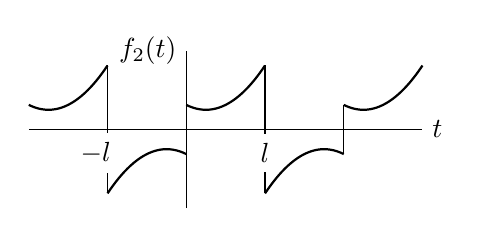
\begin{tikzpicture}
\draw(-2,0)--(3,0)node[right]{$t$};
\draw(0,-1)--(0,1)node[left]{$f_2(t)$};
%
\draw[thick,domain=0:1,smooth] plot ({\x},{0.25+(\x-0.25)*(\x-0.25)});
\draw[thick,domain=0:1,smooth] plot ({\x+2},{0.25+(\x-0.25)*(\x-0.25)});
\draw[thick,domain=0:1,smooth] plot ({\x-2},{0.25+(\x-0.25)*(\x-0.25)});
\draw[thick,domain=0:1,smooth] plot ({-\x},{-0.25-(\x-0.25)*(\x-0.25)});
\draw[thick,domain=0:1,smooth] plot ({2-\x},{-0.25-(\x-0.25)*(\x-0.25)});
%
\draw(-1,0.8125)--(-1,-0.8125);
\draw(1,0.8125)--(1,-0.8125);
\draw(0,0.3125)--(0,-0.3125);
\draw(2,0.3125)--(2,-0.3125);
%
\draw(1,0)node[shift={(0,-0.3)},fill=white]{$l$};
\draw(-1,0)node[shift={(-0.15,-0.3)},fill=white]{$-l$};
\end{tikzpicture}
\caption*{(پ) تفاعل $f(t)$ کی طاق دوری توسیع}
\end{subfigure}%
\caption{دوری توسیع}
\label{شکل_فوریئر_دوری_توسیع}
\end{figure}
%===================
\ابتدا{مثال}\شناخت{مثال_فوریئر_تکونی_دھڑکن}\quad تکونی دھڑکن\\
درج ذیل تکونی دھڑکن کی نصف حلقہ اتساع کریں (شکل \حوالہ{شکل_مثال_فوریئر_تکونی_دھڑکن})۔
\begin{align*}
f(t)=
\begin{cases}
\frac{2k}{l}t&0<t<\frac{l}{2}\\
\frac{2k}{l}(l-t)&\frac{l}{2}<t<l
\end{cases}
\end{align*}
%
\begin{figure}
\centering
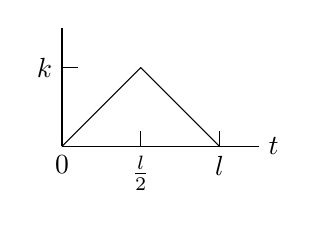
\begin{tikzpicture}
\draw(0,0)--(2.5,0)node[right]{$t$};
\draw(0,0)--(0,1.5);
%
\draw(0,0)node[below]{$0$}--(1,1)--(2,0);
\draw(1,0)node[below]{$\frac{l}{2}$}--++(0,0.2);
\draw(2,0)node[below]{$l$}--++(0,0.2);
\draw(0,1)node[left]{$k$}--++(0.2,0);
\end{tikzpicture}
\caption{تکونی دھڑکن (مثال \حوالہ{مثال_فوریئر_تکونی_دھڑکن})}
\label{شکل_مثال_فوریئر_تکونی_دھڑکن}
\end{figure}

حل:مساوات \حوالہ{مساوات_فوریئر_نصف_حلقہ_توسیع_جفت_عددی_سر} سے درج ذیل ملتا ہے۔
\begin{align*}
a_0&=\frac{1}{l}\big[\frac{2k}{l}\int_0^{\frac{l}{2}}t\,\dif t+\frac{2k}{l}\int_{\frac{l}{2}}^{l}(l-t)\,\dif t\big]=\frac{k}{2}\\
a_n&=\frac{2}{l}\big[\frac{2k}{l}\int_0^{\frac{l}{2}}t\cos \frac{n\pi}{l}t\,\dif t+\frac{2k}{l}\int_{\frac{l}{2}}^{l}(l-t)\cos \frac{n\pi}{l}t\,\dif t\big]
\end{align*}
تکمل بالحصص لیتے  سے
\begin{align*}
\int_0^{\frac{l}{2}}t\cos \frac{n\pi}{l}t\,\dif t&=\left. \frac{lt}{n\pi}\sin \frac{n\pi}{l}t\right|_0^{\frac{l}{2}}-\frac{1}{n\pi}\int_0^{\frac{l}{2}} \sin \frac{n\pi}{l}t\,\dif t\\
&=\frac{l^2}{2n\pi}\sin \frac{n\pi}{2}+\frac{l^2}{n^2\pi^2}(\cos \frac{n\pi}{2}-1)
\end{align*}
ملتا ہے۔اسی طرح تکمل بالحصص سے
\begin{align*}
\int_{\frac{l}{2}}^{l}(l-t)\cos \frac{n\pi}{l}t\,\dif t=-\frac{l^2}{2n\pi}\sin\frac{n\pi}{2}-\frac{l^2}{n^2\pi^2}(\cos n\pi-\cos \frac{n\pi}{2})
\end{align*}
ملتا ہے۔ان نتائج سے
\begin{align*}
a_n=\frac{4k}{n^2\pi^2}(2\cos \frac{n\pi}{2}-\cos n\pi-1)
\end{align*}
یعنی
\begin{align*}
a_2&=-\frac{16k}{2^2\pi^2},\quad a_6=-\frac{16k}{6^2\pi^2},\quad a_{10}=-\frac{16k}{10^2\pi^2},\cdots\\
a_n&=0,\quad n\ne 2,6,10,14,\cdots
\end{align*}
حاصل ہوتا ہے۔یوں تکونی دھڑکن  \عددی{f(t)} کی پہلی نصف حلقہ اتساع درج ذیل ہو گی جو \عددی{f(t)} کی دوری جفت توسیع ہے (شکل \حوالہ{شکل_مثال_فوریئر_تکونی_دھڑکن_توسیع}-الف)۔ 
\begin{align*}
f(t)=\frac{k}{2}-\frac{16k}{\pi^2}\big(\frac{1}{2^2}\cos \frac{2\pi}{l}t+\frac{1}{6^2}\cos \frac{6\pi}{l}t+\cdots\big)
\end{align*} 

اسی طرح مساوات \حوالہ{مساوات_فوریئر_نصف_حلقہ_توسیع_طاق_عددی_سر} سے
\begin{align*}
b_n=\frac{8k}{n^2\pi^2}\sin \frac{n\pi}{2}
\end{align*}
حاصل ہو گا جس سے \عددی{f(t)} کی دوسری نصف حلقہ اتساع درج ذیل حاصل ہو گی جو \عددی{f(t)} کی دوری طاق توسیع ہے (شکل \حوالہ{شکل_مثال_فوریئر_تکونی_دھڑکن_توسیع}-ب)۔
\begin{align*}
f(t)=\frac{8k}{\pi^2}\big(\frac{1}{1^2}\sin \frac{\pi}{l}t-\frac{1}{3^2}\sin \frac{3\pi}{l}t+\frac{1}{5^2}\sin \frac{5\pi}{l}t-+\cdots\big)
\end{align*}
%
\begin{figure}
\centering
\begin{subfigure}{0.5\textwidth}
\centering
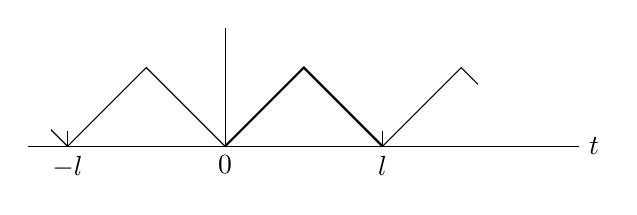
\begin{tikzpicture}
\draw(-2.5,0)--(4.5,0)node[right]{$t$};
\draw(0,0)node[below]{$0$}--(0,1.5);
%
\draw(0,0)--(-1,1)--(-2,0)--++(-45:-0.3);
\draw[thick](0,0)--(1,1)--(2,0);
\draw(2,0)--(3,1)--++(-45:0.3);
%
\draw(-2,0)node[below]{$-l$}--++(0,0.2);
\draw(2,0)node[below]{$l$}--++(0,0.2);
\end{tikzpicture}
\caption*{(الف) جفت اتساع}
\end{subfigure}
\begin{subfigure}{0.5\textwidth}
\centering
\begin{tikzpicture}
\draw(-2.5,0)--(4.5,0)node[right]{$t$};
\draw(0,0)node[below]{$0$}--(0,1.5);
%
\draw(0,0)--(-1,-1)--(-2,0)--++(-45:-0.3);
\draw[thick](0,0)--(1,1)--(2,0);
\draw(2,0)--(3,-1)--(4,0)--++(45:0.3);
%
\draw(-2,0)node[shift={(-0.2,-0.3)}]{$-l$}--++(0,0.2);
\draw(2,0)node[below]{$l$}--++(0,0.2);
\end{tikzpicture}
\caption*{(ب) طاق اتساع}
\end{subfigure}
\caption{تفاعل \عددی{f(t)} کی دوری اتساع (مثال \حوالہ{مثال_فوریئر_تکونی_دھڑکن})}
\label{شکل_مثال_فوریئر_تکونی_دھڑکن_توسیع}
\end{figure}
\انتہا{مثال}
%=========================
\حصہء{سوالات}
سوال \حوالہ{سوال_فوریئر_سائن_فوریئر_درکار_الف} تا سوال \حوالہ{سوال_فوریئر_سائن_فوریئر_درکار_ب} میں دیے گئے تفاعل \عددی{f(t)} کی فوریئر سائن تسلسل حاصل کریں اور مطابقتی دوری طاق تفاعل کی ترسیم کھینچیں۔

%=====================
\ابتدا{سوال}\شناخت{سوال_فوریئر_سائن_فوریئر_درکار_الف}\quad 
$f(t)=t,\quad (0<t<\pi)$\\
جواب:\quad
$2\sin t-\sin 2t+\tfrac{2}{3}\sin 3t-\tfrac{1}{2}\sin 4t\cdots$
\انتہا{سوال}
%===========================
\ابتدا{سوال}\quad 
$f(t)=k,\quad (0<t<l)$\\
جواب:\quad
$\tfrac{4k}{\pi}(\sin \tfrac{\pi t}{l}+\tfrac{1}{3}\sin \tfrac{3\pi t}{l}+\tfrac{1}{5}\sin \tfrac{5\pi t}{l}\cdots)$
\انتہا{سوال}
%===========================
\ابتدا{سوال}\quad
$f(t)=1-t,\quad (0<t<1)$\\
جواب:\quad
$\tfrac{1}{\pi}(2\sin \pi t+\sin 2\pi t+\tfrac{2}{3}\sin 3\pi t\cdots)$
\انتہا{سوال}
%===========================
\ابتدا{سوال}\quad
$f(t)=\cos t,\quad (0<t<\frac{\pi}{2})$\\
جواب:\quad
$\tfrac{8}{\pi}(\tfrac{1}{3}\sin 2t+\tfrac{2}{15}\sin 4t+\tfrac{3}{35}\sin 6t\cdots)$
\انتہا{سوال}
%===========================
\ابتدا{سوال}
\begin{align*}
f(t)=
\begin{cases}
t&0<t<\frac{\pi}{2}\\
\frac{\pi}{2}&\frac{\pi}{2}<t<\pi
\end{cases}
\end{align*}
جواب:\quad
$(1+\tfrac{2}{\pi})\sin t-\tfrac{1}{2}\sin 2t+(\tfrac{1}{3}-\tfrac{2}{9\pi})\sin 3t\cdots$
\انتہا{سوال}
%===========================
\ابتدا{سوال}
\begin{align*}
f(t)=
\begin{cases}
1&0<t<1\\
2-t&1<t<2
\end{cases}
\end{align*}
جواب:\quad
$\tfrac{2}{\pi}[(1+\tfrac{2}{\pi})\sin \tfrac{\pi t}{2}+\tfrac{1}{2}\sin \pi t+(\tfrac{1}{3}-\tfrac{2}{9\pi})\sin \tfrac{3\pi}{2}t\cdots]$
\انتہا{سوال}
%===========================
\ابتدا{سوال}
\begin{align*}
f(t)=
\begin{cases}
1&0<t<1\\
2&1<t<2
\end{cases}
\end{align*}
جواب:\quad
$\tfrac{2}{\pi}[3\sin \tfrac{\pi t}{2}-\sin \pi t+\sin \tfrac{3\pi t}{2}\cdots]$
\انتہا{سوال}
%===========================
\ابتدا{سوال}\شناخت{سوال_فوریئر_سائن_فوریئر_درکار_ب}
\begin{align*}
f(t)=
\begin{cases}
1-t&0<t<1\\
1&1<t<2
\end{cases}
\end{align*}
جواب:\quad
$(\tfrac{4}{\pi}-\tfrac{4}{\pi^2})\sin \tfrac{\pi t}{2}-\tfrac{1}{\pi} \sin \pi t+(\tfrac{4}{3\pi}+\tfrac{4}{9\pi^2})\sin\tfrac{3\pi t}{2}\cdots$
\انتہا{سوال}
%===========================
سوال \حوالہ{سوال_فوریئر_کوسائن_فوریئر_درکار_الف} تا سوال \حوالہ{سوال_فوریئر_کوسائن_فوریئر_درکار_ب} میں دیے گئے تفاعل \عددی{f(t)} کی فوریئر کوسائن تسلسل دریافت کریں  اور مطابقتی دوری جفت تفاعل کی ترسیم کھینچیں۔

%==================
\ابتدا{سوال}\شناخت{سوال_فوریئر_کوسائن_فوریئر_درکار_الف}\quad
$f(t)=k,\quad (0<t<l)$\\
جواب:\quad
$f(t)=k$
\انتہا{سوال}
%=======================
\ابتدا{سوال}\quad
$f(t)=t,\quad (0<t<l)$\\
جواب:\quad
$\tfrac{l}{2}-\tfrac{4l}{\pi^2}(\cos \tfrac{\pi t}{l}+\tfrac{1}{9}\cos \tfrac{3\pi t}{l}+\tfrac{1}{25}\cos \tfrac{5\pi t}{l}\cdots)$
\انتہا{سوال}
%=======================
\ابتدا{سوال}\quad
$f(t)=t^2,\quad (0<t<l)$\\
جواب:\quad
$\tfrac{l^2}{3}-\tfrac{l^2}{\pi^2}(4\cos \tfrac{\pi t}{l}-\cos \tfrac{2\pi t}{l}+\tfrac{4}{9}\cos \tfrac{3\pi t}{l}\cdots)$
\انتہا{سوال}
%=======================
\ابتدا{سوال}\quad
$f(t)=\sin t,\quad (0<t<\tfrac{\pi}{2})$\\
جواب:\quad
$\tfrac{2}{\pi}-\tfrac{4}{\pi}(\tfrac{1}{3}\cos 2t+\tfrac{1}{15}\cos 4t+\tfrac{1}{35}\cos 6t\cdots)$
\انتہا{سوال}
%=======================
\ابتدا{سوال}\quad
$f(t)=\cos t,\quad (0<t<\tfrac{\pi}{2})$\\
جواب:\quad
$\tfrac{2}{\pi}+\tfrac{4}{\pi}(\tfrac{1}{3}\cos 2t-\tfrac{1}{15}\cos 4t+\tfrac{1}{35}\cos 6t-+\cdots)$
\انتہا{سوال}
%=======================
\ابتدا{سوال}\شناخت{سوال_فوریئر_کوسائن_فوریئر_درکار_ب}\quad
$f(t)=e^t,\quad (0<t<1)$\\
جواب:\quad
$e-1-\tfrac{2}{\pi^2+1}(e+1)\cos \pi t+\tfrac{2}{4\pi^2+1}(e-1)\cos 2\pi t\cdots$
\انتہا{سوال}
%=======================
\ابتدا{سوال}\quad (فوریئر تسلسل کی مخلوط صورت، مخلوط فوریئر عددی سر)\\
کلیہ یولر \عددی{e^{i\theta}=\cos \theta +i\sin \theta}  استعمال کرتے ہوئے درج ذیل ثابت کریں
\begin{align*}
\cos nx=\frac{1}{2}(e^{inx}+e^{-inx}),\quad \sin nx=\frac{1}{2i}(e^{inx}-e^{-inx})
\end{align*}
جنہیں استعمال کرتے ہوئے فوریئر تسلسل
\begin{align*}
f(x)=a_0+\sum_{n=1}^{\infty} (a_n\cos nx+b_b\sin nx)
\end{align*}
کو
\begin{align}\label{مساوات_فوریئر_مخلوط_الف}
f(x)=c_0+\sum_{n=1}^{\infty}(c_ne^{inx}+k_ne^{-inx})
\end{align}
لکھیں جہاں \عددی{c_0=a_0}، \عددی{c_n=\tfrac{a_n-ib_n}{2}}، \عددی{k_n=\tfrac{a_n+ib_n}{2}}، \عددی{n=1,2,\cdots} ہے۔مساوات \حوالہ{مساوات_فوریئر_تسلسل_ج} استعمال کرتے ہوئے درج ذیل ثابت کریں۔
\begin{align*}
c_n=\frac{1}{2\pi}\int_{-\pi}^{\pi} f(x)e^{-inx}\dif x,\quad k_n=\frac{1}{2\pi}\int_{-\pi}^{\pi} f(x)e^{inx}\dif x,\quad n=1,2,\cdots
\end{align*}
علامت \عددی{k_n} کی جگہ علامت \عددی{c_{-n}} لکھتے  ہوئے مساوات \حوالہ{مساوات_فوریئر_مخلوط_الف} کو درج ذیل صورت میں لکھیں۔
\begin{align}\label{مساوات_فوریئر_مخلوط_ب}
f(x)=\sum_{n=-\infty}^{\infty} c_ne^{inx},\quad c_n=\frac{1}{2\pi}\int_{-\pi}^{\pi} f(x)e^{-inx}\dif x,\quad n=0,\mp 1,\mp 2,\cdots
\end{align}
اس کو \اصطلاح{مخلوط فوریئر تسلسل}\فرہنگ{فوریئر!مخلوط تسلسل}\حاشیہب{complex Fourier series}\فرہنگ{Fourier!complex form} کہتے ہیں جہاں \عددی{c_n}  کو \عددی{f(x)} کی \اصطلاح{مخلوط فوریئر عددی سر}\فرہنگ{فوریئر!مخلوط عددی سر}\حاشیہب{complex Fourier coefficients}\فرہنگ{Fourier!complex coefficients} کہتے ہیں۔
\انتہا{سوال}
%=======================
\ابتدا{سوال}
ثابت کریں کہ جفت تفاعل کی مخلوط فوریئر عددی سر حقیقی ہوں گے جبکہ طاق تفاعل کی فوریئر عددی سر خالص خیالی ہوں گے۔
\انتہا{سوال}
%=====================
سوال \حوالہ{سوال_فوریئر_مخلوط_درکار_الف} تا سوال \حوالہ{سوال_فوریئر_مخلوط_درکار_ب} میں دوری عرصہ \عددی{2\pi} کی دی گئی تفاعل \عددی{f(x)} کی مخلوط فوریئر تسلسل دریافت کریں۔مخلوط فوریئر تسلسل سے حقیقی فوریئر تسلسل حاصل کرتے ہوئے  گزشتہ حاصل کردہ تسلسل کے ساتھ موازنہ کریں۔

%====================
\ابتدا{سوال}\شناخت{سوال_فوریئر_مخلوط_درکار_الف}\quad (سوال \حوالہ{سوال_فوریئر_جفت_طاق_معلوم_الف})
$f(x)=\abs{x}\quad (-\pi<x<\pi)$\\
جواب:\quad
$\sum\limits_{\substack{ n=-\infty\\ n\ne 0}}^{\infty} {\frac{-2 e^{inx}}{\pi n^2}}$
\انتہا{سوال}
%======================
\ابتدا{سوال}\quad (سوال \حوالہ{سوال_فوریئر_جفت_طاق_معلوم_الف_بعد_ب})
$f(x)=x\quad (-\pi<x<\pi)$\\
جواب:\quad
$\sum\limits_{\substack{ n=-\infty\\ n\ne 0}}^{\infty} {\frac{i (-1)^n e^{inx}}{n}}$
\انتہا{سوال}
%======================
\ابتدا{سوال}\quad (سوال \حوالہ{سوال_فوریئر_جفت_طاق_معلوم_الف_بعد_پ})
$f(x)=x^2\quad (-\pi<x<\pi)$\\
جواب:\quad
$\sum\limits_{\substack{ n=-\infty\\ n\ne 0}}^{\infty} {\frac{2(-1)^n e^{inx}}{n^2}}$
\انتہا{سوال}
%======================
\ابتدا{سوال}\شناخت{سوال_فوریئر_مخلوط_درکار_ب}\quad (سوال \حوالہ{سوال_فوریئر_جفت_طاق_معلوم_الف_بعد_ت})
$f(x)=e^x\quad (-\pi<x<\pi)$\\
جواب:\quad
$\frac{\sinh \pi}{\pi}\sum\limits_{-\infty}^{\infty} (-1)^n \frac{1+i n}{1+n^2}e^{inx}$
\انتہا{سوال}
%======================

\حصہ{فوریئر عددی سر کا بغیر تکمل حصول}
آپ نے دیکھا کہ  بعض اوقات پیچیدہ تکملات حل کرنے کے بعد نسبتاً سادہ فوریئر عددی سر \عددی{a_n} اور \عددی{b_n} حاصل ہوتے ہیں۔اس سے سوال پیدا ہوتا ہے کہ آیا عددی سر حاصل کرنے کا کوئی آسان طریقہ بھی ہے؟ جس کا جواب ہے، "جی ہاں"۔ ہم یہاں ثابت کرتے ہیں کہ دوری کثیر رکنی تفاعل کی فوریئر عددی سر تفاعل کی اور تفاعل کی تفرقات کی چھلانگ سے حاصل کی جا سکتی ہیں۔ یوں بغیر کوئی تکمل حل کرتے ہوئے \عددی{a_n} اور \عددی{b_n} حاصل کیے جائیں گے (ماسوائے \عددی{a_0}، جس کو اب بھی تکمل کے ذریعہ حاصل کیا جائے گا)۔

نقطہ \عددی{x_0} پر تفاعل \عددی{g(x)} کی \اصطلاح{چھلانگ}\فرہنگ{چھلانگ}\حاشیہب{jump}\فرہنگ{jump} \عددی{j} سے مراد \عددی{x_0} پر \عددی{g(x)} کی دائیں ہاتھ حد اور بائیں ہاتھ حد میں فرق ہے (حصہ \حوالہ{حصہ_فوریئر_یولر_کلیات}) یعنی:
\begin{align}
j=g(x_0+0)-g(x_0-0)
\end{align}
یوں اوپر کو چھلانگ مثبت چھلانگ ہو گی جبکہ نیچے کو چھلانگ منفی چھلانگ ہو گی (شکل \حوالہ{شکل_فوریئر_تفاعل_کی_چھلانگ})۔
\begin{figure}
\centering
\begin{subfigure}{0.5\textwidth}
\centering
\begin{tikzpicture}
\draw(0,0)--(2,0)node[below]{$t$};
\draw(0,0)--(0,1.2);
\draw(0,0.25) to [out=30,in=180]++(0.5,0.5)coordinate(kA)++(0,0.5) to [out=-30,in=135]++(1.5,-0.7);
\draw[-stealth](kA)++(0,0.1)--++(0,0.3);
\end{tikzpicture}
\caption*{(الف) مثبت چھلانگ}
\end{subfigure}%
\begin{subfigure}{0.5\textwidth}
\centering
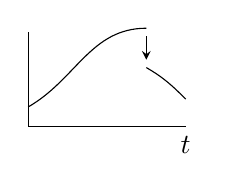
\begin{tikzpicture}
\draw(0,0)--(2,0)node[below]{$t$};
\draw(0,0)--(0,1.2);
\draw(0,0.25) to [out=30,in=180]++(1.5,1)coordinate(kA)++(0,-0.5) to [out=-30,in=135]++(0.5,-0.4);
\draw[-stealth](kA)++(0,-0.1)--++(0,-0.3);
\end{tikzpicture}
\caption*{(ب) منفی چھلانگ}
\end{subfigure}%
\caption{تفاعل کی چھلانگ}
\label{شکل_فوریئر_تفاعل_کی_چھلانگ}
\end{figure}

فرض کریں کہ دوری تفاعل \عددی{f(x)} جس کا عددی عرصہ \عددی{2\pi} ہے کو وقفہ \عددی{-\pi<x<\pi} میں کثیر رکنی \عددی{p-1}، \نقطے، \عددی{p_m} سے ظاہر کیا جا سکتا ہے (مثلاً شکل \حوالہ{شکل_فوریئر_کثیر_رکنی_روپ})۔
\begin{figure}
\centering
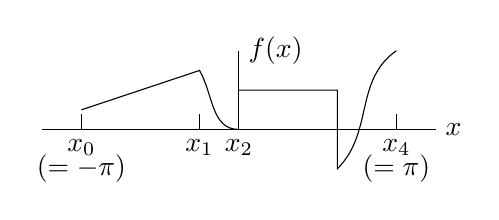
\begin{tikzpicture}
\draw(-2.5,0)--(2.5,0)node[right]{$x$};
\draw(0,0)--(0,1)node[right]{$f(x)$};
%
\draw(-2,0.25)--(-0.5,0.75) to [out=-60,in=180](0,0)++(0,0.5)--(1.25,0.5)--++(0,-1) to [out=45,in=-145](2,1);
\draw(-2,0)node[below]{$x_0$}node[shift={(0,-0.5)}]{$(=-\pi)$}--++(0,0.2);
\draw(-0.5,0)node[below]{$x_1$}--++(0,0.2);
\draw(0,0)node[below]{$x_2$};
\draw(2,0)node[below]{$x_4$}node[shift={(0,-0.5)}]{$(=\pi)$}--++(0,0.2);
\end{tikzpicture}
\caption{کثیر رکنی روپ کی مثال (مساوات \حوالہ{مساوات_فوریئر_کثیر_رکنی_روپ_الف}) جہاں $m=4$ ہے}
\label{شکل_فوریئر_کثیر_رکنی_روپ}
\end{figure}
%
\begin{align}\label{مساوات_فوریئر_کثیر_رکنی_روپ_الف}
f(x)=
\begin{cases}
p_1(x)&x_0<x<x_1,\quad (x_0=-\pi)\\
p_2(x)& x_1<x<x_2\\
\vdots&\\
p_3(x)& x_{m-1}<x<x_m \quad (x_m=\pi)
\end{cases}
\end{align}
یوں \عددی{x_0}، \نقطے، \عددی{x_m} پر تفاعل \عددی{f} کی چھلانگ اور اس کی تفرق \عددی{f'}، \عددی{f''}، \نقطے  کی چھلانگ ہو سکتی ہیں جنہیں ہم درج ذیل سے ظاہر کرتے ہیں۔
\begin{gather}
\begin{aligned}\label{مساوات_فوریئر_چھلانگ_الف}
j_s&=\text{\RL{$x_s$ پر $f$ کی چھلانگ}}\\
j'_s&=\text{\RL{$x_s$ پر $f'$ کی چھلانگ}}\\
j''_s&=\text{\RL{$x_s$ پر $f''$ کی چھلانگ}}\\
\vdots\\
j^{n}_s&=\text{\RL{$x_s$ پر $f^{(n)}$ کی چھلانگ}}\\
\end{aligned}
\quad \quad (s=1,2,\cdots,m)
\end{gather}
ظاہر ہے کہ اگر \عددی{x_s} پر \عددی{f} استمراری ہو تب \عددی{x_s} پر \عددی{j_s=0} ہو گا۔ایسا ہی \عددی{f'}، \عددی{f''}،\نقطے  کے لئے بھی کہا جا سکتا ہے۔یوں مساوات \حوالہ{مساوات_فوریئر_چھلانگ_الف} میں کئی \عددی{j_s}، \عددی{j'_s}،\نقطے صفر قیمتیں ہو سکتی ہیں۔

%================
\ابتدا{مثال}\شناخت{مثال_فوریئر_چھلانگ_الف}\quad تفاعل کی چھلانگ اور اس کی تفرق کی چھلانگیں\\
تفاعل \عددی{f(x)} 
\begin{align*}
f=
\begin{cases}
0& -\pi<x<0\\
x^2&\phantom{-}0<x<\pi
\end{cases}
\end{align*}
اور اس کی تفرقات \عددی{f'}، \عددی{f''}، \نقطے 
\begin{align*}
f'=
\begin{cases}
0\\
2x
\end{cases}
\quad 
f''=
\begin{cases}
0\\
2
\end{cases}
\quad 
f'''=0
\end{align*}
کی ترسیم شکل \حوالہ{شکل_مثال_فوریئر_چھلانگ_الف} میں کھینچی گئی ہیں  اور ان کی چھلانگیں جدول \حوالہ{جدول_مثال_فوریئر_چھلانگ_الف} میں دی گئی ہیں۔
\begin{table}
\caption{مثال \حوالہ{مثال_فوریئر_چھلانگ_الف} کی چھلانگیں}
\label{جدول_مثال_فوریئر_چھلانگ_الف}
\centering
\begin{tabular}{ccc}
& \عددی{x_1=0} پر چھلانگ & \عددی{x_2=\pi} پر چھلانگ \\
\hline
$f$  & $j_1=0$ & $j_2=-\pi^2$\\[0.5em]
$f'$  & $j'_1=0$ & $j'_2=-2\pi$\\[0.5em]
$f''$  & $j''_1=2$ & $j''_2=-2$
\end{tabular}
\end{table}
%
\begin{figure}
\centering
\begin{subfigure}{0.5\textwidth}
\centering
\begin{tikzpicture}
\draw(-1.5,0)--(2,0)node[right]{$x$};
\draw(0,0)--(0,1.5)node[right]{$f$};
%
\draw[thick,domain=0.5:1] plot ({-2+\x},{\x*\x})--(-1,0)--(0,0);
\draw[thick,domain=0:1] plot ({\x},{\x*\x});
\draw[thick,->-=0.6] (1,1)--(1,0);
\draw[thick](1,0)--(1.5,0);
%
\draw(0,1)node[left]{$\pi^2$}--++(0.2,0);
\draw(-1,0)node[below]{$-\pi$};
\draw(0,0)node[below]{$0$};
\draw(1,0)node[below]{$\pi$};
\draw(1,0.5)node[right]{$-\pi^2$};
\end{tikzpicture}
\end{subfigure}
\begin{subfigure}{0.5\textwidth}
\centering
\begin{tikzpicture}
\draw(-1.5,0)--(2,0)node[right]{$x$};
\draw(0,0)--(0,1.25)node[right]{$f'$};
%
\draw[thick] (-1,0.75)--++(-0.5,-0.375);
\draw[thick] (-1,0.75)--(-1,0)--(0,0)--(1,0.75);
\draw[thick,->-=0.6](1,0.75)--(1,0);
\draw[thick](1,0)--(1.5,0);
%
\draw(0,0.75)node[left]{$2\pi$}--++(0.2,0);
\draw(-1,0)node[below]{$-\pi$};
\draw(0,0)node[below]{$0$};
\draw(1,0)node[below]{$\pi$};
\draw(1,0.5)node[right]{$-2\pi$};
\end{tikzpicture}
\end{subfigure}
\begin{subfigure}{0.5\textwidth}
\centering
\begin{tikzpicture}
\draw(-1.5,0)--(2,0)node[right]{$x$};
\draw(0,0)--(0,1)node[right]{$f''$};
%
\draw[thick] (-1.5,0.5)--(-1,0.5)--(-1,0)--(0,0);
\draw[thick,->-=0.65](0,0)--(0,0.5);
\draw[thick](0,0.5)--(1,0.5);
\draw[thick,->-=0.6](1,0.5)--(1,0);
\draw[thick](1,0)--(1.5,0);
%
\draw(0,0.5)node[left]{$2$}--++(0.2,0);
\draw(-1,0)node[below]{$-\pi$};
\draw(0,0)node[below]{$0$};
\draw(1,0)node[below]{$\pi$};
\draw(1,0.25)node[right]{$-2$};
\draw(0,0.25)node[right]{$2$};
\end{tikzpicture}
\end{subfigure}%
\caption{تفاعل اور تفاعل کی تفرقات کی چھلانگیں (مثال \حوالہ{مثال_فوریئر_چھلانگ_الف})}
\label{شکل_مثال_فوریئر_چھلانگ_الف}
\end{figure}

یاد رہے کہ  وقفہ کی ابتدا \عددی{x=-\pi} پر چھلانگیں  شمار نہیں کیے جاتے ہیں۔انہیں دوری وقفہ کی اختتام \عددی{x=\pi} پر شمار کیا جاتا ہے۔ایک ہی وقفہ پر انہیں دو مرتبہ نہیں گیا جائے گا۔
\انتہا{مثال}
%====================

مساوات \حوالہ{مساوات_فوریئر_کثیر_رکنی_روپ_الف} میں دی گئی تفاعل \عددی{f} کی فوریئر عددی سر \عددی{a_1}، \عددی{a_2}، \نقطے حاصل کرنے کی خاطر ہم یولر مساوات \حوالہ{مساوات_فوریئر_تسلسل_ج}-ب استعمال کرتے ہیں۔
\begin{align}\label{مساوات_فوریئر_بائیں_دائیں_حد_الف}
\pi a_n=\int_{-\pi}^{\pi} f \cos nx \, \dif x
\end{align}
چونکہ \عددی{f} کو مساوات \حوالہ{مساوات_فوریئر_کثیر_رکنی_روپ_الف} ظاہر کرتی ہے لہٰذا ہمیں \عددی{m} عدد تکمل کا مجموعہ
\begin{align}\label{مساوات_فوریئر_بائیں_دائیں_حد_ب}
\pi a_n=\int_{x_0}^{x_1}+\int_{x_1}^{x_2}+\cdots+\int_{x_{m-1}}^{x_m}=\sum_{s=1}^{m}\int_{x_{s-1}}^{x_s} f\cos nx\, \dif x
\end{align}
لکھنا ہو گا جہاں \عددی{x_0=-\pi} اور \عددی{x_m=\pi} ہیں۔تکمل بالحصص لیتے سے درج ذیل ملتا ہے۔
\begin{align}\label{مساوات_فوریئر_بائیں_دائیں_حد_پ}
\int_{x_{s-1}}^{x_s} f \cos nx\, \dif x=\left. \frac{f}{n} \sin nx\right|_{x_{s-1}}^{x_s}-\frac{1}{n}\int_{x_{s-1}}^{x_s} f'\sin nx\,\dif x
\end{align}
اب بائیں ہاتھ پہلی جزو میں نقطہ \عددی{x_s} پر تفاعل \عددی{f(x)} غیر استمراری ہو سکتا ہے۔ایسا ہونے کی صورت میں \عددی{x_s} پر تفاعل کی بائیں ہاتھ حد \عددی{f(x_s-0)} لینی ہو گی۔اسی طرح \عددی{x_{s-1}} پر غیر استمراری \عددی{f(x)} کی صورت میں تفاعل کی دائیں ہاتھ حد \عددی{f(x_{s-1}+0)} لینی ہو گی۔یوں  مساوات \حوالہ{مساوات_فوریئر_بائیں_دائیں_حد_پ} کا دائیں ہاتھ پہل جزو درج ذیل ہو گا۔
\begin{align*}
\frac{1}{n}[f(x_s-0)\sin nx_s-f(x_{s-1}+0)\sin nx_{s-1}]
\end{align*} 
اب مساوات \حوالہ{مساوات_فوریئر_بائیں_دائیں_حد_پ} کو مساوات \حوالہ{مساوات_فوریئر_بائیں_دائیں_حد_ب} میں پر کرتے ہوئے اور چھوٹی علامتیں \عددی{S_0=\sin nx_0}، \عددی{S_1=\sin nx_1}، \نقطے  استعمال کرتے ہوئے
\begin{multline}\label{مساوات_فوریئر_بائیں_دائیں_حد_ت}
\pi a_n=\frac{1}{n}[f(x_1-0)S_1-f(x_0+0)S_0+f(x_2-0)S_2-f(x_1+0)S_1\\
+\cdots +f(x_m-0)S_m-f(x_{m-1}+0)S_{m-1}]\\
-\frac{1}{n}\sum_{s=1}^{m}\int_{x_{s-1}}^{x_s} f' \sin nx \,\dif x
\end{multline}
ملتا ہے۔قوسین میں بند  یکساں \عددی{S} کے ارکان اکٹھا کرتے ہوئے 
\begin{multline}\label{مساوات_فوریئر_بائیں_دائیں_حد_ٹ}
-f(x_0+0)S_0+[f(x_1-0)-f(x_1+0)]S_1\\
+[f(x_2-0)-f(x_2+0)]S_2+\cdots+f(x_m-0)S_m
\end{multline}
حاصل ہوتا ہے۔ مساوات \حوالہ{مساوات_فوریئر_بائیں_دائیں_حد_ٹ} میں ہر چکور قوسین میں بند قیمت \عددی{f} کی چھلانگ ضرب \عددی{-1} کے برابر ہے۔مزید چونکہ \عددی{f} دوری ہے لہٰذا \عددی{S_0=S_m} اور \عددی{f(x_0)=f(x_m)} ہوں گے لہٰذا مساوات \حوالہ{مساوات_فوریئر_بائیں_دائیں_حد_ٹ} کے پہلے اور آخری رکن کو ملا کر \عددی{[f(x_m-0)-f(x_m+0)]S_m} لکھا جا سکتا ہے۔ یوں مساوات \حوالہ{مساوات_فوریئر_بائیں_دائیں_حد_ٹ} درج ذیل ہو گا
\begin{align*}
-j_1S_1-j_2S_2-\cdots -j_mS_m
\end{align*}
جس کو استعمال کرتے ہوئے مساوات \حوالہ{مساوات_فوریئر_بائیں_دائیں_حد_ت} کو
\begin{align}\label{مساوات_فوریئر_بائیں_دائیں_حد_ث}
\pi a_n=-\frac{1}{n}\sum_{s=1}^{m} j_s\sin nx_s-\frac{1}{n}\sum_{s=1}^{m}\int_{x_{s-1}}^{x_s}f' \sin nx\,\dif x
\end{align}
لکھا جا سکتا ہے۔یہی ترکیب دائیں ہاتھ کی تکمل پر لاگو کرتے ہوئے درج ذیل حاصل ہو گا۔
\begin{align}\label{مساوات_فوریئر_بائیں_دائیں_حد_ج}
\sum_{s=1}^{m}\int_{x_{s-1}}^{x_s} f'\sin nx\, \dif x=\frac{1}{n} \sum_{s=1}^{m}j'_s\cos nx_s+\frac{1}{n}\sum_{s=1}^{m} \int_{x_{s-1}}^{x_s} f''\cos nx\,\dif x
\end{align}
ایسا بار بار کرتے ہوئے ہمیں  تکمل کے اندر \عددی{f} کا بتدریج  زیادہ درجے کا  تفرق حاصل ہو گا۔اب چونکہ \عددی{f} کو کثیر رکنی ظاہر کرتی ہیں اور درجہ \عددی{r} کثیر رکنی کا درجہ \عددی{r+1} تفرق صفر کے برابر ہوتا ہے لہٰذا  آخر کار  کوئی تکمل باقی نہ رہے گا۔تکمل پر محدود مرتبہ یہ عمل کرنے سے ایسا ہو گا۔مساوات \حوالہ{مساوات_فوریئر_بائیں_دائیں_حد_ج} اور اس عمل کے دہرانے سے حاصل نتائج کو مساوات \حوالہ{مساوات_فوریئر_بائیں_دائیں_حد_ث} میں پر کرتے ہوئے درکار کلیہ
\begin{multline}\label{مساوات_فوریئر_چھلانگ_عددی_سر_الف}
a_n=\frac{1}{n\pi}\big[-\sum_{s=1}^{m} j_s\sin nx_s-\frac{1}{n}\sum_{s=1}^{m} j'_s \cos nx_s]\\
+\frac{1}{n^2} \sum_{s=1}^{m} j''_s\sin nx_s+\frac{1}{n^3}\sum_{s=1}^{m} j'''_s\cos nx_s--++\cdots \big]
\end{multline}
حاصل ہوتا ہے جہاں \عددی{n=1,2,\cdots} ہے (اور \عددی{a_0} کو پہلی کی طرح تکمل کے ذریعہ حاصل کیا جائے گا)۔ بالکل اسی طرح یولر مساوات \حوالہ{مساوات_فوریئر_تسلسل_ج}-پ استعمال کرتے ہوئے \عددی{b_n} کا کلیہ
\begin{multline}\label{مساوات_فوریئر_چھلانگ_عددی_سر_ب}
b_n=\frac{1}{n\pi}\big[\sum_{s=1}^{m} j_s\cos nx_s-\frac{1}{n}\sum_{s=1}^{m} j'_s \sin nx_s]\\
-\frac{1}{n^2} \sum_{s=1}^{m} j''_s\cos nx_s+\frac{1}{n^3}\sum_{s=1}^{m} j'''_s\sin nx_s+--++\cdots \big]
\end{multline}
حاصل ہو گا۔

غلطیوں سے بچنے کی خاطر \عددی{f(x)} اور اس کی تفرقات کی ترسیم کھینچ کر چھلانگوں کو (مثال \حوالہ{مثال_فوریئر_چھلانگ_الف} کی طرح) جدول میں لکھنا  سود مند ثابت ہوتا ہے۔

%===========================
\ابتدا{مثال}\شناخت{مثال_فوریئر_چکور_چھلانگ}\quad دوری چکور موج\\
دوری چکور موج \عددی{f(x)} کی فوریئر عددی سر دریافت کریں (شکل \حوالہ{شکل_مثال_فوریئر_چکور_چھلانگ})۔
\begin{align*}
f(x)=
\begin{cases}
-k&-\pi<x<0\\
\phantom{-}k&\phantom{-}0<x<\pi
\end{cases}
\end{align*}
%
\begin{figure}
\centering
\begin{tikzpicture}
\draw(-2.5,0)--(2.5,0)node[right]{$x$};
\draw(0,-1.5)--(0,1.5);
%
\draw(-2,1)--++(1,0)--++(0,-2);
\draw[thick](-1,-1)--++(1,0);
\draw[thick,->-=0.75](0,-1)--++(0,2);
\draw[thick](0,1)--++(1,0);
\draw[thick,->-=0.25](1,1)--++(0,-2);
\draw(1,-1)--++(1,0);
%
\draw(0,1)node[left]{$k$};
\draw(0,-1)node[right]{$-k$};
\draw(-1,0)node[shift={(-0.3,-0.2)}]{$-\pi$};
\draw(0,0)node[shift={(-0.3,-0.2)}]{$0$};
\draw(1,0)node[shift={(0.3,-0.2)}]{$\pi$};
\draw(0,0.5)node[right]{$j_1$};
\draw(1,0.5)node[right]{$j_2$};
\end{tikzpicture}
\caption{چکور موج کی چھلانگیں (مثال \حوالہ{مثال_فوریئر_چکور_چھلانگ})}
\label{شکل_مثال_فوریئر_چکور_چھلانگ}
\end{figure}

حل: چونکہ \عددی{f'=0} ہے لہٰذا صرف \عددی{f} کی چھلانگیں پائی جاتی ہیں۔یہ چھلانگیں جدول \حوالہ{جدول_مثال_فوریئر_چکور_چھلانگ} میں دی گئی ہیں۔
\begin{table}[!htbp]
\caption{چکور موج کی چھلانگیں (مثال \حوالہ{مثال_فوریئر_چکور_چھلانگ})}
\label{جدول_مثال_فوریئر_چکور_چھلانگ}
\centering
\begin{tabular}{c|c|c}
\hline
& \عددی{x_1=0} پر چھلانگ& \عددی{x_2=\pi} پر چھلانگ\\
\hline
 $f$&$ j_1=2k$&$j_2=-2k$\\
\hline
\end{tabular}
\end{table}
\عددی{f} طاق ہے لہٰذا مساوات \حوالہ{مساوات_فوریئر_چھلانگ_عددی_سر_ب} سے فوریئر عددی سر حاصل کرتے ہیں۔
\begin{align*}
b_n&=\frac{1}{n\pi}[j_1\cos nx_1+j_2\cos nx_2]=\frac{1}{n\pi}[2k\cos 0-2k\cos n\pi]\\
&=\frac{2k}{n\pi}(1-\cos n\pi)=
\begin{cases}
\frac{4k}{n\pi}& \text{\RL{طاق $n$}}\\
0&\text{\RL{جفت $n$}}
\end{cases}
\quad\quad \text{\RL{(مثال \حوالہ{مثال_فوریئر_چکور_موج} دیکھیں)}}
\end{align*}
\انتہا{مثال}
%=============================
\ابتدا{مثال}\شناخت{مثال_فوریئر_چھلانگ_ب}\quad
مثال \حوالہ{مثال_فوریئر_چھلانگ_الف} میں دی گئی تفاعل کی فوریئر تسلسل حاصل کریں۔\\
حل: تکمل سے \عددی{a_0} حاصل کرتے ہیں۔
\begin{align*}
a_0=\frac{1}{2\pi}\int_0^{\pi}x^2\dif x=\frac{\pi^2}{6}
\end{align*}
مساوات \حوالہ{مساوات_فوریئر_چھلانگ_عددی_سر_الف} سے
\begin{align*}
a_n=\frac{1}{n\pi}[\pi^2\sin n\pi+\frac{2\pi}{n}\cos n\pi+\frac{1}{n^2}(2\sin 0-2\sin n\pi)]=\frac{2}{n^2}\cos n\pi
\end{align*}
یعنی \عددی{a_1=-\tfrac{2}{1^2}}، \عددی{a_2=\tfrac{2}{2^2}}، \عددی{a_3=-\tfrac{2}{3^2}}، \نقطے ملتے ہیں۔مساوات \حوالہ{مساوات_فوریئر_چھلانگ_عددی_سر_ب} سے
\begin{align*}
b_n&=\frac{1}{n\pi}[-\pi^2\cos n\pi+\frac{2\pi}{n}\sin n\pi-\frac{1}{n^2}(2\cos 0-2\cos n\pi)]\\
&=-\frac{\pi}{n}\cos n\pi+\frac{2}{n^2 \pi}(\cos n\pi-1)
\end{align*}
یعنی
\begin{align*}
b_1=\pi-\frac{4}{\pi},\quad b_2=-\frac{\pi}{2},\quad b_3=\frac{\pi}{3}-\frac{4}{3^2\pi},\quad b_4=-\frac{\pi}{4},\cdots
\end{align*}
ملتے ہیں۔یوں فوریئر تسلسل در ذیل ہو گی۔
\begin{align*}
f(x)=\frac{\pi^2}{6}-2\cos x+(\pi-\frac{4}{\pi})\sin x+\frac{1}{2}\cos 2x-\frac{\pi}{2}\sin 2x+\cdots
\end{align*}
\انتہا{مثال}
%==============================

\حصہء{سوالات}
%========================
\ابتدا{سوال}\quad مثال \حوالہ{مثال_فوریئر_چھلانگ_ب} کو عمومی طریقہ سے حل کریں۔آپ دیکھیں گے کہ عمومی طریقہ بہت لمبا ہو گا۔
\انتہا{سوال}
%========================
\ابتدا{سوال}\quad یولر مساوات \حوالہ{مساوات_فوریئر_تسلسل_ج}-پ استعمال کرتے ہوئے مساوات \حوالہ{مساوات_فوریئر_چھلانگ_عددی_سر_ب} حاصل کریں۔
\انتہا{سوال}
%==========================
\ابتدا{سوال}\quad ثابت کریں کہ \عددی{T} دوری عرصہ کی تفاعل کے لئے مساوات \حوالہ{مساوات_فوریئر_چھلانگ_عددی_سر_الف} اور مساوات \حوالہ{مساوات_فوریئر_چھلانگ_عددی_سر_ب} درج ذیل صورت اختیار کرتی ہیں۔
\begin{multline}\label{مساوات_فوریئر_چھلانگ_عددی_سر_پ}
a_n=\frac{1}{n\pi}\big[-\sum_{s=1}^{m}j_s\sin K_n t_s-\frac{1}{K_n}\sum_{s=1}^{m}j'_s\cos K_n t_s\quad \quad \quad(K_n=\frac{2n\pi}{T})\\
+\frac{1}{K_n^2}\sum_{s=1}^{m}j''_s\sin K_nt_s+\frac{1}{K_n^3}\sum_{s=1}^{m}j'''_s\cos K_nt_s--++\cdots\big]
\end{multline}
%
\begin{multline}\label{مساوات_فوریئر_چھلانگ_عددی_سر_ت}
b_n=\frac{1}{n\pi}\big[\sum_{s=1}^{m}j_s\cos K_n t_s-\frac{1}{K_n}\sum_{s=1}^{m}j'_s\sin K_n t_s\\
-\frac{1}{K_n^2}\sum_{s=1}^{m}j''_s\cos K_nt_s+\frac{1}{K_n^3}\sum_{s=1}^{m}j'''_s\sin K_nt_s+--++\cdots\big]
\end{multline}


\انتہا{سوال}
%==================
سوال \حوالہ{سوال_فوریئر_چھلانگ_سے_حل_الف} تا سوال \حوالہ{سوال_فوریئر_چھلانگ_سے_حل_ب} میں فوریئر تسلسل کو مساوات \حوالہ{مساوات_فوریئر_چھلانگ_عددی_سر_الف} تا مساوات \حوالہ{مساوات_فوریئر_چھلانگ_عددی_سر_ت} کی مدد سے حاصل کریں۔

%=========================
\ابتدا{سوال}\شناخت{سوال_فوریئر_چھلانگ_سے_حل_الف}\quad سوال \حوالہ{سوال_فوریئر_تسلسل_دریافت_کریں_الف} تا سوال \حوالہ{سوال_فوریئر_تسلسل_دریافت_کریں_ت}
\انتہا{سوال}
%===========================
\ابتدا{سوال}\quad سوال \حوالہ{سوال_فوریئر_درکار_چھلانگ_الف} تا سوال \حوالہ{سوال_فوریئر_درکار_چھلانگ_ب}
\انتہا{سوال}
%===========================
\ابتدا{سوال}\quad سوال \حوالہ{سوال_فوریئر_درکار_چھلانگ_پ} تا سوال \حوالہ{سوال_فوریئر_درکار_چھلانگ_ت}
\انتہا{سوال}
%===========================
\ابتدا{سوال}\شناخت{سوال_فوریئر_چھلانگ_سے_حل_ب}\quad سوال \حوالہ{سوال_فوریئر_درکار_چھلانگ_ٹ} تا سوال \حوالہ{سوال_فوریئر_درکار_چھلانگ_ث}
\انتہا{سوال}
%===========================
سوال \حوالہ{سوال_فوریئر_چھلانگ_کثیر_رکنی_الف} تا سوال \حوالہ{سوال_فوریئر_چھلانگ_کثیر_رکنی_ب} کی فوریئر سائن تسلسل کو مساوات \حوالہ{مساوات_فوریئر_چھلانگ_عددی_سر_الف} تا مساوات \حوالہ{مساوات_فوریئر_چھلانگ_عددی_سر_ت} کی مدد سے حاصل کریں۔

%===================
\ابتدا{سوال}\شناخت{سوال_فوریئر_چھلانگ_کثیر_رکنی_الف}\quad
$f(x)=x^2+2x+1 \quad (0<x<\pi)$\\
جواب:\quad
$(2\pi-\tfrac{4}{\pi}+4)\sin x-(2+\pi)\sin 2x+(\tfrac{2}{3}+\tfrac{28}{27\pi}+\tfrac{4}{3})\sin 3x\cdots$
\انتہا{سوال}
%=====================
\ابتدا{سوال}\quad 
$f(x)=x^3\quad (0<x<1)$\\
جواب:\quad
$\tfrac{2}{\pi^3}(\pi^2-6)\sin \pi x-\tfrac{(4\pi^2-6)}{4\pi^3}\sin 2\pi x+\tfrac{2(9\pi^2-6)}{27\pi^3}\sin3\pi x\cdots$
\انتہا{سوال}
%======================
\ابتدا{سوال}\quad
$f(x)=x(1-x) \quad (0<x<1)$\\
جواب:\quad
$\tfrac{8}{\pi^3}(\sin \pi t+\tfrac{1}{3^3}\sin 3\pi t+\tfrac{1}{5^3}\sin 5\pi t+\cdots)$
\انتہا{سوال}
%=====================
\ابتدا{سوال}\شناخت{سوال_فوریئر_چھلانگ_کثیر_رکنی_ب}\quad
$f(x)=x(x^2-1) \quad (0<x<1)$\\
جواب:\quad
$\tfrac{1}{\pi^3}(-12\sin \pi t+\tfrac{3}{2}\sin 2\pi t-\tfrac{4}{9}\sin 3\pi t+\tfrac{3}{16}\sin 4\pi t\cdots)$
\انتہا{سوال}
%=====================
\ابتدا{سوال}\quad 
تفاعل \عددی{f(x)=x^3,\quad (0<x<l)} کی فوریئر کوسائن تسلسل کو مساوات \حوالہ{مساوات_فوریئر_چھلانگ_عددی_سر_پ} کی مدد سے حاصل کریں۔\\
جواب:\quad
$\tfrac{l^3}{4}+l^3(\tfrac{24}{\pi^4}-\tfrac{6}{\pi^2})\cos\tfrac{\pi t}{l}+\tfrac{3l^3}{2\pi^2}\cos \tfrac{2\pi t}{l}\cdots$
\انتہا{سوال}
%======================

\حصہ{جبری ارتعاش}
تفرقی مساوات میں فوریئر تسلسل اہم ثابت ہوتے ہیں۔آئیں ایک اہم عملی مسئلہ پر غور کریں جس کی سادہ تفرقی مساوات پائی جاتی ہے۔ (جزوی تفرقی مساوات والے مسائل پر اگلے باب میں غور کیا جائے گا۔) 
\begin{figure}
\centering
\begin{tikzpicture}
\pgfmathsetmacro{\width}{0.9}
\pgfmathsetmacro{\height}{0.9}
\node[circle,fill=gray,inner sep=2.5mm] (b) at (0,0) {} ++(-0.37,0)node[left]{کمیت} ++(0.74,0) node[right]{$m$};
\draw[decorate,decoration={coil,aspect=0.3, segment length=1.7mm, amplitude=3mm}] (0,3) -- (b)node[pos=0.5,shift={(-0.8,0)}]{اسپرنگ}node[pos=0.5,shift={(0.6,0)}]{$k$}; 
\fill [pattern = north east lines] (-1,3) rectangle (1,3.2);
\draw[thick] (-1,3) -- (1,3);
\draw[dashed](0.9,0)--(1.4,0);
\draw[-latex] (1.3,0)--++(0,-1.2)node[pos=0.5,right]{$r(t)$};
%dashboard
\draw[] (b)--++(0,-0.8)coordinate(c);
\draw[ultra thick](c) ++(-\width/2+0.1,0)--++(\width-0.2,0);
\draw[thick] (c)++(-\width/2,\height/3)--++(0,-\height)--++(\width,0)--++(0,\height);
\draw(c)++(-\width/2,0)node[left]{\RL{روک (جاذب)}};
\draw(c)++(\width/2,0)node[right]{$c$};
\end{tikzpicture}
\caption{اسپرنگ اور کمیت کے نظام کی جبری ارتعاش۔}
\label{شکل_فوریئر_اسپرنگ_کمیت_جبری_ارتعاش}
\end{figure}

ہم حصہ \حوالہ{حصہ_سادہ_دو_جبری_ارتعاش} سے جانتے ہیں کہ اسپرنگ کے ساتھ جڑی  ہوئی کمیت \عددی{m} (شکل \حوالہ{شکل_فوریئر_اسپرنگ_کمیت_جبری_ارتعاش}) کی جبری ارتعاش کی سادہ تفرقی مساوات
\begin{align}\label{مساوات_فوریئر_جبری_ارتعاش_الف}
m\ddot{y}+c\dot{y}+ky=r(t)
\end{align}
ہے جہاں \عددی{c} تقصیری مستقل اور \عددی{k} مقیاس لچک ہے۔بیرونی قوت سائن یا کوسائن تفاعل ہونے اور غیر صفر تقصیری مستقل کی صورت میں برقرار حالت ہارمونی ارتعاش پیدا ہو گی  جس کی تعدد بیرونی قوت کی تعدد ہو گی۔   

ایسی قوت \عددی{r(t)} جو نہ خالص سائن تفاعل ہو اور نہ ہی خالص کوسائن تفاعل ہو بلکہ کسی اور شکل کی دوری تفاعل ہونے کی صورت میں ہم دیکھیں گے کہ برقرار حالت حل کئی ہارمونی ارتعاش کا مجموعہ ہو گا جس میں \عددی{r(t)} کی تعدد اور اس کی مضرب تعدد  پائی جائیں گی۔اگر ان تمام تعدد میں سے کوئی تعدد، نظام کی قدرتی تعدد کے قریب ہو تب عین ممکن ہے کہ،  بیرونی قوت کی رد عمل میں، نظام کی حرکت میں اسی تعدد کا حصہ غالب ہو گا۔ہارمونی ارتعاش اور گمک کے بارے میں نہ جانتے ہوئے یہ عمل حیرت انگیز ثابت ہو گا۔آئیں ایک مثال سے اس حقیقت کو سمجھیں۔

%=========================
\ابتدا{مثال}\شناخت{مثال_فوریئر_جبری_ارتعاش}\quad غیر سائن نما جبری قوت سے پیدا ارتعاش\\
مساوات \حوالہ{مساوات_فوریئر_جبری_ارتعاش_الف} میں \عددی{m=\SI{1}{\kilo\gram}}، \عددی{k=\SI{25}{\kilo\gram\per\second\squared}}، \عددی{c=\SI{0.02}{\kilo\gram\per\second}} لینے سے درج ذیل حاصل ہو گا جہاں \عددی{r(t)} کی اکائی \عددی{\si{\kilogram\meter\per\second\squared}} ہو گی۔
\begin{align}\label{مساوات_فوریئر_جبری_ارتعاش_مثال_الف}
\ddot{y}+0.02\dot{y}+25y=r(t)
\end{align}
اب فرض کریں کہ جبری قوت \عددی{r(t)} درج ذیل ہے جس کو شکل \حوالہ{شکل_مثال_فوریئر_جبری_ارتعاش} میں دکھایا گیا ہے۔برقرار حالت حل دریافت کریں۔
\begin{align*}
r(t)=
\begin{cases}
\phantom{-}t+\frac{\pi}{2}& -\pi<t<0\\
-t+\frac{\pi}{2}&\phantom{-}0<t<\pi
\end{cases}
\quad\quad  r(t+2\pi)=r(t)
\end{align*}
%
\begin{figure}
\centering
\begin{tikzpicture}
\draw(-1.5,0)--(1.5,0)node[right]{$t$};
\draw(0,-1.2)--(0,1.5)node[right]{$r(t)$};
\draw[thick](-1,-1)--++(-0.25,0.5);
\draw[thick](-1,-1)--(0,1)--(1,-1)--++(0.25,0.5);
%
\draw(0,1)node[left]{$\tfrac{\pi}{2}$}--++(0.2,0);
\draw(0,-1)node[left]{$-\tfrac{\pi}{2}$}--++(0.2,0);
\draw(-1,0)node[below]{$-\pi$}--++(0,0.2);
\draw(1,0)node[below]{$\pi$}--++(0,0.2);
\end{tikzpicture}
\caption{تکونی قوت (مثال \حوالہ{مثال_فوریئر_جبری_ارتعاش})}
\label{شکل_مثال_فوریئر_جبری_ارتعاش}
\end{figure}

حل:ہم \عددی{r(t)} کو فوریئر کوسائن تسلسل
\begin{align}\label{مساوات_فوریئر_جبری_ارتعاش_مثال_ب}
r(t)=\frac{4}{n^2\pi}\cos nt=\frac{4}{\pi} \big(\cos t+\frac{1}{3^2}\cos 3t+\frac{1}{5^2}\cos 5t+\cdots\big)
\end{align}
سے ظاہر کرتے ہیں۔اب ہم درج ذیل تفرقی مساوات پر غور کرتے ہیں جس کا دایاں ہاتھ فوریئر تسلسل (مساوات \حوالہ{مساوات_فوریئر_جبری_ارتعاش_مثال_ب}) کا ایک رکن ہے۔
\begin{align}\label{مساوات_فوریئر_جبری_ارتعاش_مثال_پ}
\ddot{y}+0.02\dot{y}+25y=\frac{4}{n^2\pi}\cos nt\quad \quad \quad (n=1,23,\cdots)
\end{align}
ہم حصہ \حوالہ{حصہ_سادہ_دو_جبری_ارتعاش} سے جانتے ہیں کہ درج بالا تفرقی مساوات کا برقرار حالت حل درج ذیل صورت کا ہو گا۔
\begin{align}\label{مساوات_فوریئر_جبری_ارتعاش_مثال_ت}
y_n=A_n\cos nt+B_n\sin nt
\end{align}
مساوات \حوالہ{مساوات_فوریئر_جبری_ارتعاش_مثال_ت} کو مساوات \حوالہ{مساوات_فوریئر_جبری_ارتعاش_مثال_پ} میں پر کرتے ہوئے
\begin{align}\label{مساوات_فوریئر_جبری_ارتعاش_مثال_ٹ}
A_n=\frac{4(25-n^2)}{n^2\pi D}, \quad B_n=\frac{0.08}{n\pi D}, \quad  \quad D=(25-n^2)^2+(0.02n)^2
\end{align}
ملتا ہے۔چونکہ تفرقی مساوات \حوالہ{مساوات_فوریئر_جبری_ارتعاش_مثال_الف} خطی ہے لہٰذا ہم توقع کرتے ہیں کہ اس کا برقرار حالت حل 
\begin{align}\label{مساوات_فوریئر_جبری_ارتعاش_مثال_ث}
y=y_1+y_3+y_5+\cdots
\end{align}
ہو گا جہاں مساوات \حوالہ{مساوات_فوریئر_جبری_ارتعاش_مثال_ت} \عددی{y_n} دیتی ہے۔درحقیقت آپ حاصل مساوات \حوالہ{مساوات_فوریئر_جبری_ارتعاش_مثال_ث} کو مساوات \حوالہ{مساوات_فوریئر_جبری_ارتعاش_مثال_پ} میں پر کرتے ہوئے ثابت کر سکتے ہیں کہ یہ تفرقی مساوات کا درست حل ہے۔

مساوات \حوالہ{مساوات_فوریئر_جبری_ارتعاش_مثال_ٹ} سے مساوات \حوالہ{مساوات_فوریئر_جبری_ارتعاش_مثال_ت}  کا حیطہ
\begin{align*}
C_n=\sqrt{A_n^2+B_n^2}=\frac{A}{n^2\pi\sqrt{D}}
\end{align*}
حاصل ہوتا ہے  جس کی چند اعدادی قیمتیں درج ذیل ہیں۔
\begin{align*}
C_1&=0.0530\\
C_3&=0.0088\\
C_5&=0.5100\\
C_7&=0.0011\\
C_9&=0.0003
\end{align*}
\عددی{n=5} پر \عددی{D} کی قیمت نہایت کم ملتی ہے  جس سے \عددی{C_5} کی قیمت اتنی زیادہ حاصل ہوتی ہے کہ مساوات \حوالہ{مساوات_فوریئر_جبری_ارتعاش_مثال_ث} میں \عددی{y_5} غالب جزو  ہے۔ یوں برقرار حالت حرکت تقریباً ہارمونی ہو گا جس کی تعدد جبری قوت کی تعدد کی پانچ گنا ہے (شکل \حوالہ{شکل_مثال_فوریئر_جبری_ارتعاش_رد_عمل})۔
\begin{figure}
\centering
\begin{tikzpicture}
\draw(0,0)--(5,0)node[right]{$t$};
\draw(0,0)--(0,2.5);
%
\draw(0,1)--(2,-1)--(4,1)--++(0.4,-0.4)node[right]{$r(t)$};
\draw[domain=0:355,samples=200] plot ({4/360*\x},{4/3.142*(0.167*cos(\x)+0.028*cos(2*\x)+1.6*sin(5*\x))});
\draw(0,0)node[below]{$0$};
\draw(2,0)node[shift={(0,-0.3)},fill=white]{$\pi$}--++(0,0.2);
\draw(4,0)node[shift={(0,-0.3)},fill=white]{$2\pi$}--++(0,0.2);
\draw[stealth-](3.5,1.5)to [out=45,in=180]++(0.5,0.5)node[right]{\RL{برقرار حال حرکت}};
\end{tikzpicture}
\caption{داخلی قوت اور برقرار حالت رد عمل (مثال \حوالہ{مثال_فوریئر_جبری_ارتعاش})}
\label{شکل_مثال_فوریئر_جبری_ارتعاش_رد_عمل}
\end{figure}
\انتہا{مثال}
%======================

\حصہء{سوالات}
سوال \حوالہ{سوال_فوریئر_جبری_ارتعاش_الف} تا سوال \حوالہ{سوال_فوریئر_جبری_ارتعاش_ب} میں تفرقی مساوات \عددی{\ddot{y}+\omega^2\y=r(t)} کی عمومی حل دریافت کریں۔

%===============
\ابتدا{سوال}\شناخت{سوال_فوریئر_جبری_ارتعاش_الف}\quad 
$r(t)=\sin t,\quad \omega =0.5,0.7,0.9,1.1,1.5,2.0,10$\\
جواب:\quad
$y=C_1\cos \omega t+C_2\sin \omega t+A(\omega)\sin t,\quad A(\omega)=\tfrac{1}{\omega^2-1}$\\
$A(0.5)=-1.33,A(0.7)=-0.2, A(0.9)=-5.3,A(1.1)=4.8,A(1.5)=0.8,$\\
 $A(2)=0.33, A(10)=0.01$
\انتہا{سوال}
%=====================
\ابتدا{سوال}\quad 
$r(t)=\cos \alpha t+\cos \beta t, \quad (\omega^2 \ne \alpha^2,\beta^2)$\\
جواب:\quad
$C_1\cos \omega t+C_2\sin \omega t+\tfrac{(\omega^2-\alpha^2)\cos \beta t+(\omega^2-\beta^2)\cos \alpha t}{\omega^4-(\alpha^2+\beta^2)\omega^2+\alpha^2\beta^2}$
\انتہا{سوال}
%==================
\ابتدا{سوال}\quad
$r(t)=\sin t+\sin 3t, \quad w=0.9, 2.9$\\
جواب:\quad
\begin{align*}
y=C_1\cos \omega t+C_2\sin \omega t+\tfrac{\sin t}{\omega^2-1^2}+\tfrac{\sin 3t}{\omega^2-3^2}\\
y_{(\omega=0.9)}=C_1\cos \omega t+C_2\sin \omega t-5.26\sin t-0.122\sin 3t\\
y_{(\omega=2.9)}=C_1\cos \omega t+C_2\sin \omega t+0.135\sin t-0.164\sin 3t
\end{align*}
\انتہا{سوال}
%======================
\ابتدا{سوال}\quad
$r(t)=\sum\limits_{s=1}^{N} a_n \cos nt,\quad \abs{\omega}\ne 1,2,\cdots,N$\\
جواب:\quad
$y=C_1\cos \omega t+C_2\sin \omega t+\sum\limits_{n=1}^{N} \frac{a_n}{\omega^2-n^2}\cos nt$
\انتہا{سوال}
%=======================
\ابتدا{سوال}\quad
$r(t)=\sum\limits_{s=1}^{N} b_n \sin nt,\quad \abs{\omega}\ne 1,2,\cdots,N$\\
جواب:\quad
$y=C_1\cos \omega t+C_2\sin \omega t+\sum\limits_{n=1}^{N} \frac{b_n}{\omega^2-n^2}\sin nt$
\انتہا{سوال}
%=======================
\ابتدا{سوال}\quad
\begin{align*}
r(t)=
\begin{cases}
-1&-\pi<t<0\\
\phantom{-}1&\phantom{-}0<t<\pi
\end{cases}
\quad\quad r(t+2\pi)=r(t), \quad \abs{\omega}\ne 1,3,5,\cdots
\end{align*}
جواب:\quad
$y=C_1\cos \omega t+C_2\sin \omega t+\tfrac{4\sin t}{1\pi(\omega^2-1^2)}+\tfrac{4\sin 3t}{3\pi(\omega^2-3^2)}+\tfrac{4\sin 5t}{5\pi(\omega^2-5^2)}\cdots$
\انتہا{سوال}
%=======================
\ابتدا{سوال}\quad 
$r(t)=t,\quad (-\pi<t<\pi), r(t+2\pi)=r(t),\abs{\omega}\ne 1,2,3,\cdots$\\
جواب:\quad
$y=C_1\cos \omega t+C_2\sin \omega t+\sum\limits_{n=1}^{\infty} \tfrac{2(-1)^{n+1}}{n(\omega^2-n^2)}\sin nt$
\انتہا{سوال}
%======================
\ابتدا{سوال}\شناخت{سوال_فوریئر_جبری_ارتعاش_ب}\quad 
$r(t)=t^2,\quad (-\pi<t<\pi), r(t+2\pi)=r(t),\abs{\omega}\ne 0, 1,2,\cdots$\\
جواب:\quad
$y=C_1\cos \omega t+C_2\sin \omega t+C_3+\sum\limits_{n=1}^{\infty}\tfrac{4(-1)^n}{n^2(\omega^2-n^2)}\cos nx$
\انتہا{سوال}
%======================
سوال \حوالہ{سوال_فوریئر_برقرار_حل_چاہیے_الف} تا سوال \حوالہ{سوال_فوریئر_برقرار_حل_چاہیے_ب} میں \عددی{\ddot{y}+c\dot{y}+y=r(t)} جہاں \عددی{c>0} ہے کی برقرار حالت حل دریافت کریں۔

%================
\ابتدا{سوال}\شناخت{سوال_فوریئر_برقرار_حل_چاہیے_الف}\quad
$r(t)=\cos t$\\
جواب:\quad
$y=\tfrac{\sin t}{c}$
\انتہا{سوال}
%=======================
\ابتدا{سوال}\quad
$r(t)=\sin 3t$\\
جواب:\quad
$y=-\tfrac{8}{9c^2+8^2}\sin 3t-\tfrac{3}{9c^2+8^2}\cos 3t$
\انتہا{سوال}
%=======================
\ابتدا{سوال}\quad
$r(t)=\cos nt$\\
جواب:\quad
$y=\tfrac{nc\sin nt-(n^2-1)\cos nt}{(n^2-1)^2+n^2c^2}$
\انتہا{سوال}
%=======================
\ابتدا{سوال}\quad
$r(t)=\sin nt$\\
جواب:\quad
$y=\tfrac{-nc\cos nt-(n^2-1)\sin nt}{(n^2-1)^2+n^2c^2}$
\انتہا{سوال}
%=======================
\ابتدا{سوال}\شناخت{سوال_فوریئر_برقرار_حل_چاہیے_ب}
\begin{align*}
r(t)=
\begin{cases}
\pi+t&-\pi<t<0\\
\pi-t&\phantom{-}0<t<\pi
\end{cases}
\quad \quad r(t+2\pi)=r(t)
\end{align*}
جواب:\quad
$y=\tfrac{\pi}{2}+\sum\limits_{n=1}^{\infty}\tfrac{4}{n^2\pi[(n^2-1)^2+n^2c^2]}[nc\sin nt-(n^2-1)\cos nt]$
\انتہا{سوال}
%===============================
\ابتدا{سوال}\quad سلسلہ وار \عددی{RLC} دور کو  \عددی{E(t)} داخلی دباو مہیا کی جاتی ہے۔اس دور میں برقی رو \عددی{I(t)} دریافت کریں۔
\begin{align*}
E(t)=
\begin{cases}
-10&-\pi<t<0\\
\phantom{-}10&\phantom{-}0<t< \pi
\end{cases}
\quad \quad E(t+2\pi)=E(t)
\end{align*}
%
\begin{figure}
\centering
\begin{tikzpicture}
\draw(0,0) to [american voltage source,l={$E(t)$}]++(0,\y) to [resistor,l={\SI{1}{\ohm}}]++(\x,0) to [short,i={$I(t)$}]++(\x/4,0) to [inductor,l={$\SI{1}{\henry}$}]++(\x,0) to [capacitor,l={$\SI{0.01}{\farad}$}]++(0,-\y) to [short](0,0);
\end{tikzpicture}
\end{figure}
جواب:\quad
$I=\sum\limits_{n=1}^{\infty}\tfrac{40}{\pi[n^4-199n^2+10^4]}[n\sin nt-(n^2-10^2)\cos nt]$
\انتہا{سوال}
%==================================

\حصہ{تقریب بذریعہ تکونی کثیر رکنی۔ مکعب خلل}
فرض کریں کہ \عددی{2\pi} دوری عرصہ کی تفاعل \عددی{f(x)} کو فوریئر تسلسل کی صورت میں لکھنا ممکن ہے۔اس تسلسل کی پہلی \عددی{N} ارکان کا جزوی مجموعہ، \عددی{f(x)} کی تقریب ہو گی۔
\begin{align}\label{مساوات_فوریئر_تقریب_الف}
f(x)\approx a_0+\sum\limits_{n=1}^{N}(a_n\cos nx+b_n\sin nx)
\end{align}
تکونی کثیر رکنی کی عددی سر یوں منتخب کی جا سکتے ہیں  کہ یہ تفاعل پر ٹھیک بیٹھے۔یہاں سوال پیدا ہوتا ہے کہ آیا \عددی{f(x)} کو تکونی کثیر رکنی
\begin{align}\label{مساوات_فوریئر_تقریب_ب}
F(x)=\alpha_0+\sum\limits_{n=1}^{N} (\alpha_n \cos nx+\beta_n\sin nx)
\end{align}
سے ظاہر کرنے کی "بہترین" تقریب مساوات \حوالہ{مساوات_فوریئر_تقریب_الف} دیتی ہے جہاں دونوں تقریب میں \عددی{N} یکساں ہے۔بہترین تقریب  میں کم سے کم "خلل" پایا جاتا ہے۔

ظاہر ہے کہ ہمیں پہلے  فیصلہ کرنا ہو گا کہ، تقریب میں  خلل، سے ہمارا کیا مراد ہے۔ ہم خلل کی ایسی تعریف منتخب کرتے ہیں جو پورے وقفہ \عددی{-\pi\le x\le \pi} پر \عددی{f} اور \عددی{F} کی ایک سا ہونے کی ناپ ہو۔شکل \حوالہ{شکل_فوریئر_خلل_تقریب} میں \عددی{f} کو \عددی{F} سے ظاہر کیا گیا ہے جو بہتر تقریب ہے لیکن نقطہ \عددی{x_0} پر \عددی{\abs{f-F}} کی قیمت بہت زیادہ ہے۔یوں ظاہر ہے کہ \عددی{\abs{f-F}} کی زیادہ سے زیادہ قیمت کو خلل کہنا موزوں نہ ہو گا۔ہم خلل کی تعریف درج ذیل لیتے ہیں
\begin{align}\label{مساوات_فوریئر_تقریب_پ}
E=\int_{-\pi}^{\pi} (f-F)^2\,\dif x
\end{align}
جس وقفہ \عددی{-\pi \le x\le \pi} پر تفاعل \عددی{F} کی، تفاعل \عددی{f} کے لحاظ سے،  \اصطلاح{کل مکعب خلل}\فرہنگ{خلل!کل مکعب}\حاشیہب{total square error}\فرہنگ{error!total square} کہلاتا ہے۔چونکہ مکعب کبھی بھی منفی نہیں ہو سکتا ہے لہٰذا \عددی{E \ge 0} ہو گا۔
\begin{figure}
\centering
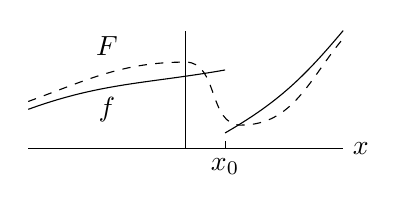
\begin{tikzpicture}
%\draw[thick] (-2,0) grid (2,1.5);
%\draw[thin,gray,step=0.1](-2,0) grid (2,1.5);
%
\draw(-2,0)--(2,0)node[right]{$x$};
\draw(0,0)--(0,1.5);
%
\draw(-2,0.5) to [out=20,in=-170](0.5,1)(0.5,0.2) to [out=30,in=-130](2,1.5);
\draw[dashed](-2,0.6) to [out=20,in=180](0,1.1) to [out=0,in=180](0.7,0.3) to [out=0,in=-130] (2,1.4);
%
\draw(-1,0.5)node{$f$};
\draw(-1,1.3)node{$F$};
\draw(0.5,0)node[below]{$x_0$}--++(0,0.1);
\end{tikzpicture}
\caption{تقریب کی خلل}
\label{شکل_فوریئر_خلل_تقریب}
\end{figure}

ہم مقررہ \عددی{N} کے لئے مساوات \حوالہ{مساوات_فوریئر_تقریب_ب} کے ایسے عددی سر دریافت کرنا چاہتے ہیں کہ حاصل \عددی{E} کمترین ہو۔ہم مساوات \حوالہ{مساوات_فوریئر_تقریب_پ} کو درج ذیل صورت میں لکھ سکتے ہیں۔
\begin{align}\label{مساوات_فوریئر_تقریب_ت}
E=\int_{-\pi}^{\pi} f^2\dif x-2\int_{-\pi}^{\pi} fF\,\dif x+\int_{-\pi}^{\pi} F^2\,\dif x
\end{align}
درج بالا کی آخری تکمل میں مساوات \حوالہ{مساوات_فوریئر_تقریب_ب} پر کرتے ہوئے حاصل تکملات کو حصہ \حوالہ{حصہ_فوریئر_یولر_کلیات} کی طرح حل کرنے سے درج ذیل ملتا ہے۔ 
\begin{align*}
\int_{-\pi}^{\pi} F^2\dif x=\pi(2\alpha_0^2+\alpha_1^2+\cdots+\alpha_N^2+\beta_1^2+\cdots+\beta_N^2)
\end{align*}
مساوات \حوالہ{مساوات_فوریئر_تقریب_ب} کو  مساوات \حوالہ{مساوات_فوریئر_تقریب_ت} کی دائیں ہاتھ دوسری تکمل میں پر کرنے سے   یولر کلیات (مساوات \حوالہ{مساوات_فوریئر_تسلسل_ج}) کے تکمل حاصل ہوتے ہیں جن سے درج ذیل لکھا جا سکتا ہے۔
\begin{align*}
\int_{-\pi}^{\pi} fF\,\dif x=\pi(2\alpha_0a_0+\alpha_1a_1+\cdots+\alpha_Na_N+\beta_1b_1+\cdots+\beta_Nb_N)
\end{align*}
یوں مساوات \حوالہ{مساوات_فوریئر_تقریب_ت} سے درج ذیل حاصل ہوتا ہے۔
\begin{multline}\label{مساوات_فوریئر_تقریب_ٹ}
E=\int_{-\pi}^{\pi} f^2\dif x-2\pi\big[2\alpha_0a_0+\sum\limits_{n=1}^{N}(\alpha_na_n+\beta_nb_n)\big]\\
+\pi\big[2\alpha_0^2+\sum\limits_{n=1}^{N}(\alpha_n^2+\beta_n^2)\big]
\end{multline}
مساوات \حوالہ{مساوات_فوریئر_تقریب_ب} میں \عددی{\alpha_n=a_n} اور \عددی{\beta_n=b_n} لینے سے  مساوات \حوالہ{مساوات_فوریئر_تقریب_ٹ} سے حاصل کل مکعب خلل درج ذیل ملتا ہے۔
\begin{align}\label{مساوات_فوریئر_تقریب_ث}
E^*=\int_{-\pi}^{\pi} f^2\dif x-\pi\big[2a_0^2+\sum\limits_{n=1}^{N}(a_n^2+b_n^2)\big]
\end{align}
مساوات \حوالہ{مساوات_فوریئر_تقریب_ث} کو مساوات \حوالہ{مساوات_فوریئر_تقریب_ٹ} سے منفی کرتے ہوئے
\begin{align*}
E-E^*=\pi\big\{2(\alpha_0-a_0)^2+\sum\limits_{n=1}^{N}[(\alpha_n-a_n)^2+(\beta_n-b_n)^2]\big\}
\end{align*}
ملتا ہے۔چونکہ بائیں ہاتھ تمام قیمتیں مکعب ہیں جو کبھی بھی منفی نہیں ہو سکتے ہیں لہٰذا 
\begin{align*}
E-E^*\ge 0\quad \implies \quad E\ge E^*
\end{align*}
ہو گا اور \عددی{E=E^*} صرف اور صرف اس صورت ہو گا جب \عددی{\alpha_0=a_0}، \نقطے، \عددی{\beta_N=b_N} ہوں۔اس سے درج ذیل مسئلہ ثابت ہوتا ہے۔

%=============================
\ابتدا{مسئلہ}\quad (کمترین مکعب خلل)\\
وقفہ \عددی{-\pi \le x\le \pi} پر تفاعل \عددی{f} کے لحاظ سے \عددی{F} [مساوات \حوالہ{مساوات_فوریئر_تقریب_ب}، مقررہ \عددی{N}] کی کل مکعب خلل صرف اور صرف اس صورت کم سے کم ہو گی جب مساوات \حوالہ{مساوات_فوریئر_تقریب_ب} میں \عددی{F} کے عددی سر، \عددی{f} کی  مطابقتی فوریئر عددی سر ہوں۔ کل مکعب خلل کی کم سے کم قیمت مساوات \حوالہ{مساوات_فوریئر_تقریب_ث} دے گی۔
\انتہا{مسئلہ}
%=======================

ہم مساوات \حوالہ{مساوات_فوریئر_تقریب_ث} سے دیکھتے ہیں کہ \عددی{N} بڑھانے سے \عددی{E^*} بڑھتا نہیں بلکہ گھٹ سکتا ہے۔یوں زیادہ \عددی{N} لینے سے  \عددی{f} کی فوریئر تسلسل سے حاصل جزوی مجموعہ کا کل مکعب خلل کم ہو گا اور بہتر تقریب حاصل ہو گی۔

چونکہ \عددی{E^*\ge 0} ہے  اور مساوات \حوالہ{مساوات_فوریئر_تقریب_ث} ہر \عددی{N} کے لئے درست ہے لہٰذا مساوات \حوالہ{مساوات_فوریئر_تقریب_ث} سے 
\begin{align}\label{مساوات_فوریئر_بیسل_غیر_مساوات}
2a_0^2+\sum\limits_{n=1}^{\infty} (a_n^2+b_n^2)\le \frac{1}{\pi}\int_{-\pi}^{\pi} f^2(x)\,\dif x
\end{align}
لکھا جا سکتا ہے جو \اصطلاح{ بیسل غیر مساوات}\فرہنگ{بیسل!غیر مساوات}\حاشیہب{Bessel inequality}\فرہنگ{Bessel!inequality} کہلاتی\حاشیہد{یہ ثابت کیا جا سکتا ہے کہ ایسا تفاعل \عددی{f} کے لئے مساوات \حوالہ{مساوات_فوریئر_بیسل_غیر_مساوات} میں برابری کی علامت لکھنا بھی درست ہو گا۔مساوات \حوالہ{مساوات_فوریئر_بیسل_غیر_مساوات} میں برابری کی علامت استعمال کرنے سے \اصطلاح{پارسیوال مماثل} حاصل ہو گی۔}\فرہنگ{پارسیوال مماثل}\فرہنگ{Parseval's identity} ہے۔مساوات \حوالہ{مساوات_فوریئر_بیسل_غیر_مساوات} کسی بھی تفاعل \عددی{f}، جس کے لئے درج بالا تکمل معین ہو، کی فوریئر عددی سر کے لئے درست ہو گا۔

%=====================
\حصہء{سوالات}

%===============
\ابتدا{سوال}\شناخت{سوال_فوریئر_مکعب_خلل_الف}\quad تفاعل \عددی{f(x)=x,\quad (-\pi<x<\pi),\quad f(x+\pi)=f(x)} کے لئے ایسا \عددی{F(x)} (مساوات \حوالہ{مساوات_فوریئر_تقریب_ب}) دریافت کریں کہ کل مکعب خلل (مساوات \حوالہ{مساوات_فوریئر_تقریب_پ}) کمترین ہو۔ \\
جواب:\quad
$F(x)=\tfrac{2}{1}\sin x-\tfrac{2}{2}\sin 2x+\tfrac{2}{3}\sin 3x-+\cdots +\tfrac{2(-1)^{N+1}}{N}\sin Nx$
\انتہا{سوال}
%====================
\ابتدا{سوال}\quad \عددی{N=1,2,3,4} کے لئے سوال \حوالہ{سوال_فوریئر_مکعب_خلل_الف} میں کمتر مکعب خلل دریافت کریں۔ایسا \عددی{N} دریافت کریں کہ \عددی{E^*\le 0.42} ہو۔\\
جواب:\quad
$E(1)=8.104,\,E(2)=4.96,\,E(3)=3.57,\,E(4)=2.78,\quad N=30$
\انتہا{سوال}
%=====================
\ابتدا{سوال}\quad ثابت کریں کہ \عددی{N} کو بتدریج بڑھانے سے کل کمتر مکعب خلل  (مساوات \حوالہ{مساوات_فوریئر_تقریب_ث}) بتدریج گھٹتی ہے۔ 
\انتہا{سوال}
%=====================
\ابتدا{سوال}\quad  تفاعل \عددی{f(x)=x^2,\quad (-\pi<x<\pi),\quad f(x+\pi)=f(x)} کے لئے ایسا \عددی{F(x)} (مساوات \حوالہ{مساوات_فوریئر_تقریب_ب}) دریافت کریں کہ کل مکعب خلل کمترین ہو۔کمتر مکعب خلل کو \عددی{N=1,2,3,4} کے لئے حاصل کریں۔\\
جواب:
\begin{align*}
F&=\tfrac{\pi^2}{3}-4[\tfrac{1}{1^2}\cos x-\tfrac{1}{2^2}\cos 2x+\tfrac{1}{3^2}\cos 3x-+\cdots +\tfrac{(-1)^{N+1}}{N^2}\cos Nx]\\
E^* &=\tfrac{2\pi^5}{5}-\pi(\tfrac{2\pi^4}{9}+16+1+\tfrac{16}{81}+\tfrac{1}{16}+\cdots)
\end{align*}
\انتہا{سوال}
%============================

\حصہ{فوریئر تکمل}
دوری تفاعل پر مبنی مسئلوں کو نمٹنے کے لئے فوریئر تسلسل بہترین اوزار ہے۔ہم چاہیں گے کہ اس  کو عمومی شکل دیں تا کہ یہ \اصطلاح{غیر دوری تفاعل} کے لئے بھی کارآمد ہو۔ 

ہم ابتدا دو سادہ دوری تفاعل \عددی{f_T} سے کرتے ہیں۔ہم \عددی{T\to \infty} کرتے ہوئے دیکھتے ہیں کہ کیا ہوتا ہے۔اس کے بعد ہم دوری عرصہ \عددی{T} کی کسی بھی دوری تفاعل \عددی{f_T} پر غور کرتے ہوئے \عددی{T\to \infty} کریں گے۔ان کو جواز بناتے ہوئے ہم مسئلہ فوریئر تکمل پیش کریں گے۔
%===============
\ابتدا{مثال}\شناخت{مثال_فوریئر_تکمل_الف}\quad
درج ذیل تفاعل پر غور کریں جس کا دوری عرصہ \عددی{T>2} ہے (شکل \حوالہ{شکل_مثال_فوریئر_تکمل_الف})۔
\begin{align*}
f_T(x)=
\begin{cases}
0&-\frac{T}{2}<x<-1\\
1&-1<x<1\\
0&\phantom{-}1<x<\frac{T}{2}
\end{cases}
\end{align*}
دوری عرصہ \عددی{T\to \infty} کرنے سے درج ذیل تفاعل \عددی{f(x)} 
\begin{align*}
f(x)=\lim_{T\to \infty} f_T(x)=
\begin{cases}
1&-1<x<1\\
0&\text{\RL{بصورت دیگر}}
\end{cases}
\end{align*}
%
\begin{figure}
\centering
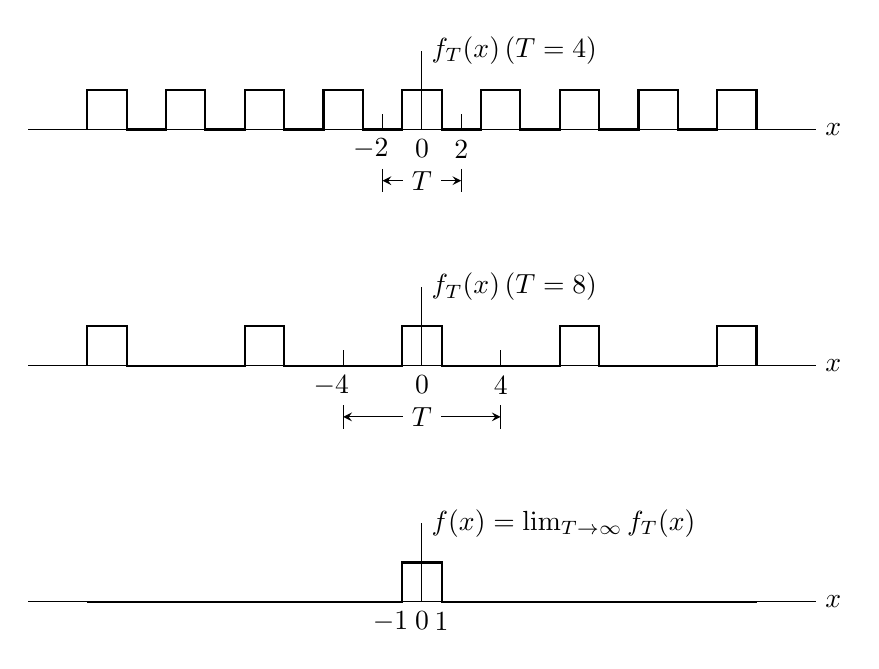
\begin{tikzpicture}
\pgfmathsetmacro{\k}{0.5}
\draw(-5,0)--(5,0)node[right]{$x$};
\draw(0,0)node[below]{$0$}--(0,1)node[right]{$f_T(x)\, (T=4)$};
\draw[thick](0,\k)--++(\k/2,0)--++(0,-\k)--++(\k,0)--++(0,\k)--++(\k,0)--++(0,-\k)--++(\k,0)--++(0,\k)--++(\k,0)--++(0,-\k)--++(\k,0)--++(0,\k)--++(\k,0)--++(0,-\k)--++(\k,0)--++(0,\k)--++(\k,0)--++(0,-\k);
\draw[thick](0,\k)--++(-\k/2,0)--++(0,-\k)--++(-\k,0)--++(0,\k)--++(-\k,0)--++(0,-\k)--++(-\k,0)--++(0,\k)--++(-\k,0)--++(0,-\k)--++(-\k,0)--++(0,\k)--++(-\k,0)--++(0,-\k)--++(-\k,0)--++(0,\k)--++(-\k,0)--++(0,-\k);
\draw(\k,0)node[shift={(0,-0.25)}]{$2$}--++(0,0.2);
\draw(-\k,0)node[shift={(-0.15,-0.25)}]{$-2$}--++(0,0.2);
\draw(-\k,-0.5)--++(0,-0.3)coordinate[pos=0.5](kA);
\draw(\k,-0.5)--++(0,-0.3);
\draw[stealth-stealth] (kA)--++(2*\k,0)node[pos=0.5,fill=white]{$T$};
\begin{scope}[shift={(0,-3cm)}]
\pgfmathsetmacro{\k}{0.5}
\draw(-5,0)--(5,0)node[right]{$x$};
\draw(0,0)node[below]{$0$}--(0,1)node[right]{$f_T(x)\, (T=8)$};
\draw[thick](0,\k)--++(\k/2,0)--++(0,-\k)--++(3*\k,0)--++(0,\k)--++(\k,0)--++(0,-\k)--++(3*\k,0)--++(0,\k)--++(\k,0)--++(0,-\k);
\draw[thick](0,\k)--++(-\k/2,0)--++(0,-\k)--++(-3*\k,0)--++(0,\k)--++(-\k,0)--++(0,-\k)--++(-3*\k,0)--++(0,\k)--++(-\k,0)--++(0,-\k);
\draw(2*\k,0)node[shift={(0,-0.25)}]{$4$}--++(0,0.2);
\draw(-2*\k,0)node[shift={(-0.15,-0.25)}]{$-4$}--++(0,0.2);
\draw(-2*\k,-0.5)--++(0,-0.3)coordinate[pos=0.5](kA);
\draw(2*\k,-0.5)--++(0,-0.3);
\draw[stealth-stealth] (kA)--++(4*\k,0)node[pos=0.5,fill=white]{$T$};
\end{scope}
\begin{scope}[shift={(0,-6cm)}]
\pgfmathsetmacro{\k}{0.5}
\draw(-5,0)--(5,0)node[right]{$x$};
\draw(0,0)node[below]{$0$}--(0,1)node[right]{$f(x)=\lim_{T\to \infty}f_T(x)$};
\draw[thick](0,\k)--++(\k/2,0)--++(0,-\k)--++(8*\k,0);
\draw[thick](0,\k)--++(-\k/2,0)--++(0,-\k)--++(-8*\k,0);
\draw(\k/2,0)node[shift={(0,-0.25)}]{$1$};
\draw(-\k/2,0)node[shift={(-0.15,-0.25)}]{$-1$};
\end{scope}
\end{tikzpicture}
\caption{برائے مثال \حوالہ{مثال_فوریئر_تکمل_الف}}
\label{شکل_مثال_فوریئر_تکمل_الف}
\end{figure}
حاصل ہوتا ہے جو غیر دوری ہے۔
\انتہا{مثال}
%=====================
\ابتدا{مثال}\شناخت{مثال_فوریئر_تکمل_ب}\quad
درج ذیل تفاعل کا دوری عرصہ \عددی{T} ہے (شکل \حوالہ{شکل_مثال_فوریئر_تکمل_ب})۔
\begin{align*}
f_T(x)=e^{-\abs{x}} \quad \big(-\frac{T}{2}<x<\frac{T}{2}\big),\quad f_T(x+T)=f_T(x)
\end{align*}
\عددی{T\to \infty} کرنے سے تفاعل \عددی{f(x)} حاصل ہوتا ہے جو غیر دوری ہے۔
\begin{align*}
f(x)=\lim_{T\to \infty} f_T(x)=e^{-\abs{x}}
\end{align*}
%
\begin{figure}
\centering
\begin{tikzpicture}
\draw(-4.5,0)--(5.5,0)node[right]{$x$};
\draw(0,0)node[below]{$0$}--(0,1.5)node[right]{$f_T(x)$};
%
\draw(0,1) to [out=-45,in=165]++(1,-0.5);
\draw(2,1) to [out=-45,in=165]++(1,-0.5);
\draw(4,1) to [out=-45,in=165]++(1,-0.5);
\draw(2,1) to [out=-135,in=15]++(-1,-0.5);
\draw(4,1) to [out=-135,in=15]++(-1,-0.5);
%
\draw(-2,1) to [out=-45,in=165]++(1,-0.5);
\draw(-4,1) to [out=-45,in=165]++(1,-0.5);
\draw(0,1) to [out=-135,in=15]++(-1,-0.5);
\draw(-2,1) to [out=-135,in=15]++(-1,-0.5);
%
\draw(1,0)node[below]{$\frac{T}{2}$}--++(0,0.2);
\draw(-1,0)node[below]{$-\frac{T}{2}$}--++(0,0.2);
\begin{scope}[shift={(0,-3cm)}]
\draw(-4.5,0)--(5.5,0)node[right]{$x$};
\draw(0,0)node[below]{$0$}--(0,1.5)node[right]{$f(x)$};
%
\draw(0,1) to [out=-30,in=180](5,0.1);
\draw(0,1) to [out=-150,in=0](-4.5,0.1);
\end{scope}
\end{tikzpicture}
\caption{برائے مثال \حوالہ{مثال_فوریئر_تکمل_ب}}
\label{شکل_مثال_فوریئر_تکمل_ب}
\end{figure}
\انتہا{مثال}
%===========================
ہم اب فوریئر تسلسل سے قابل ظاہر کسی بھی تفاعل \عددی{f_T(x)} جس کا دوری عرصہ \عددی{T} ہو لیتے ہیں۔مختصر علامت
\begin{align*}
w_n=\frac{2n\pi}{T}
\end{align*}
استعمال کرتے ہوئے \عددی{f_T(x)} کی فوریئر تسلسل کو 
\begin{align*}
f_T(x)=a_0+\sum\limits_{n=1}^{\infty}(a_n\cos w_nx+b_n\sin w_nx)
\end{align*}
لکھتے ہیں۔ہم دیکھنا چاہتے ہیں کہ \عددی{T\to \infty} کرنے سے کیا ہو گا۔

ہم یولر مساوات \حوالہ{مساوات_فوریئر_تسلسل_ج} میں دیے گئے \عددی{a_n} اور \عددی{b_n} استعمال کرتے ہیں اور تکمل کی متغیر کو \عددی{v} لکھتے ہیں۔ یوں درج ذیل ملتا ہے۔
\begin{multline*}
f_T(x)=\frac{1}{T}\int_{-\frac{T}{2}}^{\frac{T}{2}} f_T(v)\,\dif v+\frac{2}{T}\sum\limits_{n=1}^{\infty}\big[\cos w_nx\int_{-\frac{T}{2}}^{\frac{T}{2}}f_T(v)\cos w_nv\,\dif v\\
+\sin w_nx\int_{-\frac{T}{2}}^{\frac{T}{2}}f_T(v)\sin w_nv\,\dif v\big]
\end{multline*}
اب
\begin{align*}
w_{n+1}-w_n=\frac{2(n+1)\pi}{T}-\frac{2n\pi}{T}=\frac{2\pi}{T}
\end{align*}
ہے  جس کو ہم 
\begin{align*}
\Delta w=w_{n+1}-w_n=\frac{2\pi}{T}
\end{align*}
لکھتے ہیں۔یوں \عددی{\tfrac{2}{T}=\tfrac{\Delta w}{\pi}} ہو گا لہٰذا یہ فوریئر تسلسل  درج ذیل صورت اختیار کرے گی۔
\begin{multline}\label{مساوات_فوریئر_تکمل_الف}
f_T(x)=\frac{1}{T}\int_{-\frac{T}{2}}^{\frac{T}{2}} f_T(v)\dif v+\frac{1}{\pi}\sum\limits_{n=1}^{\infty}\big[ \cos(w_n x)\,\Delta x\int_{-\frac{T}{2}}^{\frac{T}{2}}f_T(v)\cos w_nv\,\dif v\\
+\sin (w_nx)\,\Delta w\int_{-\frac{T}{2}}^{\frac{T}{2}}f_T(v)\sin w_nv\,\dif v\big]
\end{multline}
یہ صورت کسی بھی مقررہ \عددی{T} کے لئے درست ہے جہاں \عددی{T} اختیاری وسیع لیکن محدود ہے۔

ہم اب \عددی{T\to \infty} کرتے ہیں اور فرض کرتے ہیں کہ حاصل غیر دوری تفاعل
\begin{align*}
f(x)=\lim_{T\to \infty} f_T(x)
\end{align*}
\عددی{x} محور پر \اصطلاح{قابل حتمی تکمل}\فرہنگ{تکمل!قابل حتمی تکمل}\حاشیہب{absolutely integrable}\فرہنگ{integrable!absolutely} ہے یعنی درج ذیل تکمل معین ہے۔
\begin{align}\label{مساوات_فوریئر_تکمل_ب}
\int_{-\infty}^{\infty}\abs{f(x)}\,\dif x
\end{align} 
اس طرح \عددی{\tfrac{1}{T}\to 0} ہو گا لہٰذا مساوات \حوالہ{مساوات_فوریئر_تکمل_الف} کی دائیں ہاتھ پہلا جزو صفر کے قریب تر ہو گا۔اس کے علاوہ  \عددی{{\Delta w=\tfrac{2\pi}{T}\to 0}} ہو گا لہٰذا \موٹا{بظاہر} یوں معلوم ہوتا ہے کہ لامتناہی تسلسل مساوات \حوالہ{مساوات_فوریئر_تکمل_الف} وقفہ \عددی{0} تا \عددی{\infty} پر تکمل کی صورت اختیار کرے گی جو \عددی{f(x)} کو ظاہر کرتی ہے، یعنی:
\begin{align}\label{مساوات_فوریئر_تکمل_پ}
f(x)=\frac{1}{\pi}\int\limits_{0}^{\infty}\big[\cos wx\int\limits_{-\infty}^{\infty}f(v)\cos wv\,\dif v+\sin wx\int\limits_{-\infty}^{\infty}f(v)\sin wv\,\dif v\big]\dif w
\end{align}
درج ذیل مختصر علامت متعارف کرتے ہوئے
\begin{align}\label{مساوات_فوریئر_تکمل_ت}
A(w)=\int_{-\infty}^{\infty}f(v)\cos wv\,\dif v,\quad B(w)=\int_{-\infty}^{\infty}f(v)\sin wv\,\dif v
\end{align}
مساوات \حوالہ{مساوات_فوریئر_تکمل_پ} کو
\begin{align}\label{مساوات_فوریئر_تکمل_ٹ}
f(x)=\frac{1}{\pi}\int_0^{\infty}[A(w)\cos wx+B(w)\sin wx]\dif w
\end{align}
لکھا جا سکتا ہے جس کو \عددی{f(x)} کا \اصطلاح{فوریئر تکمل}\فرہنگ{فوریئر!تکمل}\حاشیہب{ّFourier integral}\فرہنگ{Fourier!integral} کہتے ہیں۔

یہاں یہ بتلانا ضروری ہے کہ مساوات \حوالہ{مساوات_فوریئر_تکمل_الف} سے مساوات \حوالہ{مساوات_فوریئر_تکمل_پ} لکھنے کے لئے جو جواز پیش کیا گیا وہ نا کافی ہے۔درحقیقت فوریئر تسلسل میں \عددی{\Delta w\to 0} لینا تکمل کی تعریف نہیں ہے لہٰذا ایسا کرنے سے مساوات \حوالہ{مساوات_فوریئر_تکمل_الف} ہرگز حاصل نہیں ہو گا۔البتہ اس پورے عمل سے  گزرنے کے بعد  فوریئر تکمل بظاہر معقول معلوم ہوتا ہے۔فوریئر تکمل کا ثبوت اس کتاب میں پیش نہیں کیا جائے گا۔  مساوات \حوالہ{مساوات_فوریئر_تکمل_ٹ} درست ہونے کے لئے کافی شرط درج ذیل مسئلہ پیش کرتی ہے۔ 

%=================
\ابتدا{مسئلہ}\شناخت{مسئلہ_فوریئر_تکمل}\quad (فوریئر تکمل)\\
اگر \عددی{f(x)} تمام محدود قطعات پر ٹکڑوں میں استمراری (حصہ \حوالہ{حصہ_لاپلاس_بدل_الٹ_بدل_خطیت}) ہو اور اس کا ہر نقطے پر دائیں ہاتھ تفرق اور بائیں ہاتھ تفرق (حصہ \حوالہ{حصہ_فوریئر_یولر_کلیات}) پائے جاتے ہوں اور مساوات \حوالہ{مساوات_فوریئر_تکمل_ب} میں دیا گیا تکمل معین ہو تب \عددی{f(x)} کو فوریئر تکمل سے ظاہر کیا جا سکتا ہے۔جس نقطے پر \عددی{f(x)} غیر استمراری ہو وہاں فوریئر تکمل کی قیمت اس نقطے پر دائیں ہاتھ حد اور بائیں ہاتھ حد (حصہ \حوالہ{حصہ_لاپلاس_بدل_الٹ_بدل_خطیت}) کی اوسط کے برابر ہو گی۔ 
\انتہا{مسئلہ}
%=====================

\ابتدا{مثال}\شناخت{مثال_فوریئر_تکمل_چکور_دھڑکن}\quad واحد دھڑکن، سائن تکمل\\
درج ذیل تفاعل کی فوریئر تکمل حاصل کریں (شکل \حوالہ{شکل_مثال_فوریئر_تکمل_چکور_دھڑکن})۔
\begin{align*}
f(x)=
\begin{cases}
1&\abs{x}<1\\
0&\abs{x}<1
\end{cases}
\end{align*}
%
\begin{figure}
\centering
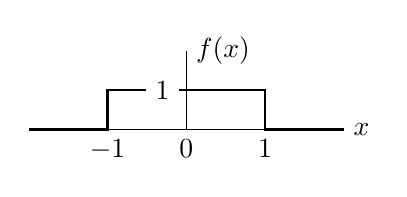
\begin{tikzpicture}
\draw(-2,0)--(2,0)node[right]{$x$};
\draw(0,0)node[below]{$0$}--(0,1)node[right]{$f(x)$};
%
\draw[thick](-2,0)--++(1,0)node[below]{$-1$}--++(0,0.5)--++(2,0)--++(0,-0.5)node[below]{$1$}--++(1,0);
\draw(0,0.5)node[shift={(-0.3,0)},fill=white]{$1$};
\end{tikzpicture}
\caption{واحد دھڑکن (مثال \حوالہ{مثال_فوریئر_تکمل_چکور_دھڑکن})}
\label{شکل_مثال_فوریئر_تکمل_چکور_دھڑکن}
\end{figure}
حل:مساوات \حوالہ{مساوات_فوریئر_تکمل_ت} سے
\begin{align*}
A(w)&=\int_{-\infty}^{\infty} f(v)\cos wv\,\dif v=\int_{-1}^{1} \cos wv\,\dif v=\left. \frac{\sin wv}{w}\right|_{-1}^{1}=\frac{2\sin w}{w}\\
B(w)&=\int_{-1}^{1}\sin wv\, \dif v=0
\end{align*}
ملتا ہے جس کو استعمال کرتے ہوئے مساوات \حوالہ{مساوات_فوریئر_تکمل_ٹ} سے درکار فوریئر تکمل حاصل کرتے ہیں۔ 
\begin{align}\label{مساوات_فوریئر_تکمل_ث}
f(x)=\frac{2}{\pi}\int_0^{\infty} \frac{\cos wx\,\sin w}{w}\dif w
\end{align}
نقطہ \عددی{x=1} پر \عددی{f(x)} کی دائیں ہاتھ حد اور بائیں ہاتھ حد کا اوسط \عددی{\tfrac{(1+0)}{2}=\tfrac{1}{2}} ہے۔یوں مساوات \حوالہ{مساوات_فوریئر_تکمل_ث} اور مسئلہ \حوالہ{مسئلہ_فوریئر_تکمل} کی مدد سے درج ذیل لکھا جا سکتا ہے۔
\begin{align}\label{مساوات_فوریئر_تکمل_ج}
\int_0^{\infty} \frac{\cos wx\,\sin w}{w}\dif w=
\begin{cases}
\frac{\pi}{2}&0\le \abs{x}< 1\\
\frac{\pi}{4}&\abs{x}=1\\
0&\abs{x}>1
\end{cases}
\end{align}
اس تکمل کو \اصطلاح{ڈرشلے غیر استمراری جزو}\فرہنگ{ڈرشلے غیر استمراری جزو}\حاشیہب{Dirichlet's discontinuous factor}\فرہنگ{Dirichlet' discontinuous factor} کہتے\حاشیہد{جرمن ریاضی دان یوہان پیٹر گستاف لیژون ڈرشلے [1805-1859]} ہیں۔آئیں \عددی{x=0} کی صورت پر غور کرتے ہیں جو خاص طور پر زیادہ اہم ہے۔مساوات \حوالہ{مساوات_فوریئر_تکمل_ج} میں \عددی{x=0} پر  کرنے سے
\begin{align}
\int_0^{\infty}\frac{\sin w}{w}\dif w=\frac{\pi}{2}
\end{align}
ملتا ہے جو درج ذیل تکمل جس کو \اصطلاح{سائن تکمل}\فرہنگ{سائن تکمل}\حاشیہب{sine integral}\فرہنگ{sine integral} کہتے ہیں 
\begin{align}\label{مساوات_فوریئر_سائن_تکمل}
\kSi(z)=\int_0^{z}\frac{\sin w}{w}\dif w
\end{align}
کی \عددی{z\to \infty} پر حد ہے جہاں \عددی{z} حقیقی ہے۔تفاعل \عددی{\kSi(z)} کو شکل میں دکھایا گیا ہے۔

فوریئر تسلسل کی صورت میں جزوی مجموعوں کی ترسیم اس دوری تفاعل کی تقریب ہوتی ہے جس کو یہ تسلسل ظاہر کرتی ہے۔ فوریئر تکمل (مساوات \حوالہ{مساوات_فوریئر_تکمل_ث}) کی صورت میں تکمل کی بالائی حد \عددی{\infty} کی جگہ عدد \عددی{a} لیتے ہوئے تفاعل کی تقریب حاصل کی جاتی ہیں۔یوں درج ذیل تکمل
\begin{align}\label{مساوات_فوریئر_گبس_الف}
\int_0^a \frac{\cos wx\sin w}{w}\dif w
\end{align}
مساوات \حوالہ{مساوات_فوریئر_تکمل_ث} اور تفاعل \عددی{f(x)} کی تقریب ہے۔تفاعل \عددی{f(x)} میں غیر استمراری نقطہ کے قریب  ارتعاش پایا جاتا ہے جس کو شکل میں دکھایا گیا ہے۔

اگرچہ ہم توقع کرتے ہیں کہ \عددی{a} کی قیمت لامتناہی کرنے سے  یہ ارتعاش ختم ہو گی، حقیقت میں ایسا نہیں ہوتا ہے بلکہ \عددی{a} کی قیمت بڑھانے سے ارتعاش  نقطہ \عددی{x=\mp 1} کے مزید قریب ہوتی ہیں۔ اس غیر متوقع کردار جو فوریئر تسلسل میں بھی پایا جاتا ہے کو \اصطلاح{مظہر گبس}\فرہنگ{مظہر گبس}\حاشیہب{Gibbs phenomenon}\فرہنگ{Gibbs phenomenon} کہتے ہیں۔ مظہر گبس\حاشیہد{جرمن ریاضی دان جوشیا ولرڈ گبس [1839-1903]} کو سمجھنے کی خاطر  ضمیمہ \حوالہ{ضمیمہ_مفید_معلومات} میں مساوات \حوالہ{مساوات_ضمیمہ_مفید_گیارہ} استعمال کرتے ہوئے مساوات \حوالہ{مساوات_فوریئر_گبس_الف} کو 
\begin{align*}
\frac{2}{\pi}\int_0^a\frac{\cos wx\sin w}{w}\dif w=\frac{1}{\pi}\int_0^a \frac{\sin(w+wx)}{w}\dif w+\frac{1}{\pi}\int_0^a 
\frac{\sin(w-wx)}{w}\dif w
\end{align*}
لکھتے ہیں۔ دائیں ہاتھ پہلی تکمل میں \عددی{w+wx=t} لیتے ہیں۔یوں \عددی{\tfrac{\dif w}{w}=\tfrac{\dif t}{t}}  اور \عددی{0\le w\le a} کا مطابقتی وقفہ \عددی{0\le t\le (x+1)a} ہو گا۔آخری تکمل میں \عددی{w-wx=t} لیتے ہیں۔یوں \عددی{\tfrac{\dif w}{w}=\tfrac{\dif t}{t}}  اور \عددی{0\le w\le a} کا مطابقتی وقفہ \عددی{0\le t\le (x-1)a} ہو گا۔چونکہ \عددی{\sin(-t)=-\sin t} ہوتا ہے لہٰذا
\begin{align*}
\frac{2}{\pi}\int_0^a\frac{\cos wx\sin w}{w}\dif w=\frac{1}{\pi}\int_0^{(x+1)a}\frac{\sin t}{t}\dif t-\frac{1}{\pi}\int_0^{(x-1)a} \frac{\sin t}{t}\dif t
\end{align*}
 لکھا جائے گا۔یوں مساوات \حوالہ{مساوات_فوریئر_سائن_تکمل} کی مدد سے
\begin{align*}
\frac{1}{\pi}\kSi{a[x+1]}-\frac{1}{\pi}\kSi(a[x-1])
\end{align*}
حاصل ہو گا لہٰذا شکل میں ارتعاش شکل کی وجہ سے پائی جاتی ہیں۔حد \عددی{a} بڑھانا، محور کی ناپ تبدیل کرنے کی مترادف ہے جس سے ارتعاش محور غیر استمراری نقطہ کے زیادہ قریب منتقل ہوتی ہیں۔
\انتہا{مثال}
%======================

\جزوحصہء{جفت اور طاق تفاعل کی فوریئر تکمل}
یہ جاننا سود مند ثابت ہوتا ہے کہ ایسا جفت یا طاق تفاعل جس کو فوریئر تکمل سے ظاہر کرنا ممکن ہو کا فوریئر تکمل عمومی تفاعل کی فوریئر تکمل سے نسبتاً آسان ہو گا۔ یہ حقیقت گزشتہ کلیات سے اخذ ہوتا ہے۔

جفت تفاعل \عددی{f(x)} کی صورت میں مساوات  \حوالہ{مساوات_فوریئر_تکمل_ت} کے تحت \عددی{B(w)=0} اور
\begin{align}\label{مساوات_فوریئر_تکمل_جفت_الف}
A(w)=2\int_0^{\infty} f(v)\cos wv\, \dif v
\end{align}
ہو گا لہٰذا مساوات \حوالہ{مساوات_فوریئر_تکمل_ٹ} درج ذیل سادہ صورت اختیار کرے گی۔
\begin{align}\label{مساوات_فوریئر_تکمل_جفت_ب}
f(x)=\frac{1}{\pi}\int_0^{\infty} A(w)\cos wx\,\dif w\quad \quad \quad (\text{\RL{جفت $f$}})
\end{align}
اسی طرح طاق تفاعل \عددی{f(x)} کی صورت میں مساوات  \حوالہ{مساوات_فوریئر_تکمل_ت} کے تحت \عددی{A(w)=0} اور
\begin{align}\label{مساوات_فوریئر_تکمل_جفت_پ}
B(w)=2\int_0^{\infty} f(v)\sin wv\, \dif v
\end{align}
ہو گا لہٰذا مساوات \حوالہ{مساوات_فوریئر_تکمل_ٹ} درج ذیل سادہ صورت اختیار کرے گی۔
\begin{align}\label{مساوات_فوریئر_تکمل_جفت_ت}
f(x)=\frac{1}{\pi}\int_0^{\infty} B(w)\sin wx\,\dif w\quad \quad \quad (\text{\RL{طاق $f$}})
\end{align}
یہ تسہیل جفت اور طاق تفاعل کی  فوریئر تسلسل کی تسہیل کی طرح ہے۔
%======================

\جزوحصہء{تخمینہ تکمل}
فوریئر تکمل کی  مدد سے کئی  تکمل کی قیمتیں حاصل کی جا سکتی ہیں۔ہم اس ترکیب کو درج ذیل مثال سے سمجھاتے  ہیں۔

%==============================
\ابتدا{مثال}\quad لاپلاس تکمل\\
درج ذیل تفاعل کی فوریئر تکمل وقفہ \عددی{x>0} پر حاصل کریں۔ (شکل \حوالہ{شکل_مثال_فوریئر_تکمل_ب} دیکھیں جہاں \عددی{k=1} ہے۔)
\begin{align*}
f(x)=e^{-kx}, \quad f(-x)=f(x)
\end{align*}
حل:چونکہ \عددی{f} جفت ہے لہٰذا مساوات \حوالہ{مساوات_فوریئر_تکمل_جفت_الف} سے 
\begin{align*}
A(w)=2\int_0^{\infty} e^{-kv}\cos wv\,\dif v
\end{align*}
حاصل ہو گا۔تکمل بالحصص لیتے ہیں۔
\begin{align*}
\int e^{-kv}\cos wv\,\dif v=-\frac{k}{k^2+w^2}e^{-kv}\big(-\frac{w}{k}\sin wv+\cos wv\big)
\end{align*}
جب \عددی{v=0} ہو تب دایاں ہاتھ \عددی{-\tfrac{k}{k^2+w^2}} کے برابر ہو گا جبکہ \عددی{v\to \infty} پر \عددی{e^{-kv}} جزو کی بنا یہ صفر کے قریب تر ہو گا۔یوں
\begin{align*}
A(w)=\frac{2k}{k^2+w^2}
\end{align*}
حاصل ہوتا ہے جس کو مساوات \حوالہ{مساوات_فوریئر_تکمل_جفت_ب} میں پر کرتے ہوئے دیے تفاعل کی فوریئر تکمل لکھتے ہیں۔
\begin{align*}
f(x)=e^{-kx}=\frac{2k}{\pi}\int_0^{\infty} \frac{\cos wx}{k^2+w^2}\dif w\quad \quad \quad (x>0,\, k>0)
\end{align*}
اس سے 
\begin{align}\label{مساوات_فوریئر_لاپلاس_تکمل_الف}
\int_0^{\infty} \frac{\cos wx}{k^2+w^2}\dif w=\frac{\pi}{2k}e^{-kx}\quad \quad \quad (x>0,\, k>0)
\end{align}
حاصل ہوتا ہے۔اسی طرح مساوات \حوالہ{مساوات_فوریئر_تکمل_جفت_ت}  استعمال کرتے ہوئے وقفہ \عددی{x>0} پر  طاق تفاعل
\begin{align*}
f(x)=e^{-kx},\quad f(-x)=-f(x), \quad \quad (k>0)
\end{align*}
 کی فوریئر تکمل سے  درج ذیل حاصل ہو گا۔
\begin{align}\label{مساوات_فوریئر_لاپلاس_تکمل_ب}
\int_0^{\infty} \frac{w\sin wx}{k^2+w^2}\dif w=\frac{\pi}{2}e^{-kx}\quad \quad \quad (x>0, k>0)
\end{align}
مساوات \حوالہ{مساوات_فوریئر_لاپلاس_تکمل_الف} اور مساوات \حوالہ{مساوات_فوریئر_لاپلاس_تکمل_ب} \اصطلاح{لاپلاس تکملات}\فرہنگ{لاپلاس!تکملات}\حاشیہب{Laplace integrals}\فرہنگ{Laplace!integrals} کہلاتے ہیں۔
\انتہا{مثال}
%=======================

\حصہء{سوالات}

